%Math template by Kaushik Srinivasan

\documentclass[11pt]{article}




%----------%
%  Basics  %
%----------%


%  Specfies basic information.
%  In the metadata section of the preamble, you can specify the subject and a list of keywords for the PDF.
%
\newcommand{\coursetitle}{MATH 110.302 - Differential Equations and Applications}
\newcommand{\lecturer}{Robert Brown}
\newcommand{\notetaker}{Kaushik Srinivasan}
\newcommand{\notetakersemail}{ksriniv4@jhu.edu}
\newcommand{\courseterm}{Fall 2018}
\newcommand{\institution}{Johns Hopkins University}


%  array provides more column styles for the tabular and array environments.
%  (http://ctan.org/pkg/array)
%
%  parskip sets block paragraphs as the default, instead of indentation.
%  (http://www.ctan.org/pkg/parskip)
%
\usepackage[margin=1in]{geometry}
\usepackage{amsmath,amssymb,amsthm,amsfonts,array,parskip}


%  Allows equation, align, gather, etc. environments to split across pages.
\allowdisplaybreaks


%  Sets date formatting to the ISO 8601 standard, YYYY-MM-DD.
\usepackage{datetime} \renewcommand{\dateseparator}{-} \yyyymmdddate


%---------%
%  Fonts  %
%---------%


%  Defines \cal for standard calligraphy, \eucal for Euler calligraphy, and \frak for Fraktur.
\usepackage{eucal}  \let\eucal\mathcal  \let\cal\CMcal  \renewcommand{\frak}{\mathfrak}


%  Removes ligatures (e.g. the connection ordinarily made between the two f's in "differentiable").
%\usepackage{microtype} \DisableLigatures{encoding=*,family=*}


%  Removes extra space after periods.




%-------------------------------%
%  Environments and Sectioning  %
%-------------------------------%


%  Defines some standard theorem environments, in both numbered and non-numbered versions. The numbering of each enviroment will be reset for each lecture.
\newcounter{lecture}       \setcounter{lecture}{0}
\newcounter{tN}[lecture]   \newcounter{dN}[lecture]
\newcounter{lN}[lecture]   \newcounter{rN}[lecture]
\newcounter{cN}[lecture]   \newcounter{eN}[lecture]
\newcounter{pN}[lecture]

\newtheorem*{theorem}{Theorem}          \newtheorem{theorem-N}[tN]{Theorem}
\newtheorem*{lemma}{Lemma}              \newtheorem{lemma-N}[lN]{Lemma}
\newtheorem*{corollary}{Corollary}      \newtheorem{corollary-N}[cN]{Corollary}
\newtheorem*{proposition}{Proposition}  \newtheorem{proposition-N}[pN]{Proposition}

\theoremstyle{definition}
\newtheorem*{definition}{Definition}    \newtheorem{definition-N}[dN]{Definition}
\newtheorem*{remark}{Remark}            \newtheorem{remark-N}[rN]{Remark}
\newtheorem*{example}{Example}          \newtheorem{example-N}[eN]{Example}
\newtheorem*{claim}{Claim}          \newtheorem{claim-N}[cN]{Claim}

% Modifies the spacing above theorem environments, which is messed up during the parskip package

\makeatletter \def\thm@space@setup{\thm@preskip=\parskip \thm@postskip=0pt} \makeatother

%Modifies the spacing above the proof environment

\makeatletter \renewenvironment{proof}[1][\proofname]{\pushQED{\qed}\normalfont
\partopsep=\z@skip \topsep=\z@skip \trivlist \item[\hskip\labelsep\itshape #1\@addpunct{.}]
\ignorespaces}{\popQED\endtrivlist\@endpefalse} \makeatother

\renewcommand{\qedsymbol}{\rule{0.7em}{0.7em}}

%Removes extra space before and after section headings

\usepackage[compact]{titlesec}

%% PICTURES AND DIAGRAMS


\usepackage[usenames, dvipsnames]{xcolor}
\definecolor{myred}{rgb}{0.9,0.2,0.2}
\definecolor{mygreen}{rgb}{0.2,0.6,0.2}
\definecolor{myblue}{rgb}{0.2,0.2,0.8}
\usepackage{caption}

%graphicx provides advanced graphics options

\usepackage{graphicx}
\graphicspath{ {./images/} }

% tikz is for drawing all sorts of pictures and diagrams

\usepackage{tikz}
\usetikzlibrary{decorations.text}
\newcommand{\tikzmark}[2]{%
    \tikz[remember picture,baseline=-2pt]
    \node[circle,red,draw,text=black,anchor=center,inner sep=1pt] (#1) {$#2$};}
\usepackage{tikz-cd}
\usepackage{pgf, pgfplots}
\usetikzlibrary{arrows,calc,decorations,decorations.markings,fadings,positioning,patterns,shapes}
\tikzset{>=latex}
\tikzstyle{mypoint}=[inner sep=0pt,outer sep=0pt,minimum size=5pt,fill,circle]
% for circled commands
\usepackage{enumitem}
%\begin{enumerate[label=\protect\circled{\arabic*}]
\newcommand*\circled[1]{\tikz[baseline=(char.base)]{\node[shape=circle,draw,inner sep=2pt] (char) {#1};}}

% HORIZONTAL LINES

\newcommand{\redhline}{\vspace{-0.1in}{\color{myred}{\rule{\textwidth}{0.02in}}}}


%------------------------%
%  Commands and Symbols  %
%------------------------%


%  Creates commands by running over a comma-separated list. For example,
%
%     \forcsvlist{\define{\newcommand}{\textbf}{bold}}{A,B}
%
%  would create
%
%     \newcommand{\boldA}{\textbf{A}}    \newcommand{\boldB}{\textbf{B}}
%
%  (http://tex.stackexchange.com/a/5776/20882)
%
\usepackage{etoolbox}
\newcommand{\define}[4]{\expandafter#1\csname#3#4\endcsname{#2{#4}}}
\forcsvlist{\define{\DeclareMathOperator}{}{}}{im,coker,rad,nil,Ann,Ass,codim,Spec,mSpec,diam,ord,Supp,supp,disc,Ob,vol,rank,Sym,Alt,Ind}
\forcsvlist{\define{\newcommand}{\mathrm}{}}{Hom,Mor,id,GL,SL,SO,SU,U,M,Mat,Ext,Tor,Res,Cor,Inf,End,Irr,Aut,Gal,lcm,tr,sign,triv,diag,Map,op,ev,act,alg,sep,unr,nr,ab}

%  Creates commands for some names of categories in the sans-serif font.
\forcsvlist{\define{\newcommand}{\mathsf}{}}{Set,Grp,Ab,CRing,Mod,Vect,Cat,Top,PreSh,Sh,Sch,Nat,Fun,Diff}

%  Creates commands for some blackboard bold letters.
\forcsvlist{\define{\newcommand}{\mathbb}{}}{N,Z,Q,R,C,F,G,T,A,B,D}


%  Saves the section symbol, paragraph symbol, Hungarian accent, and Scandanavian O in the macros \SS, \PP, \HH, and \OO, then redefines \S, \P, \H, and \O to be the corresponding blackboard bold letters.
%
\let\SS\S  \let\PP\P  \let\HH\H  \let\OO\O
\forcsvlist{\define{\renewcommand}{\mathbb}{}}{S,P,H,O}


%  latexsym defines some alternative versions of amssymb symbols.
%  (http://www.bakoma-tex.com/doc/latex/base/latexsym.pdf)
%
\usepackage{latexsym}

\usepackage{accents}
\newcommand{\Ylines}{\underaccent{\bar}{\bar{Y}}}
\newcommand{\Xlines}{\underaccent{\bar}{\bar{X}}}
\newcommand{\Lim}[1]{\raisebox{0.5ex}{\scalebox{0.8}{$\displaystyle \lim_{#1}\;$}}}
%  Defines a copyright symbol that is a bit nicer than the built-in one.
\newcommand{\mycopyrightsymbol}{\raisebox{-0.3ex}{\tikz{\node[inner sep=0pt,outer sep=0pt] at (0,0) {\textsc{c}};\draw (0,0) circle (0.18);}}}


%  Defines commands for real and complex projective space.
\newcommand{\RP}{\mathbb{R}\mathrm{P}}  \newcommand{\CP}{\mathbb{C}\mathrm{P}}


%  Defines a bordered matrix with square bracket delimiters instead of parentheses.
%  (http://tex.stackexchange.com/questions/55054)
%
\let\bbordermatrix\bordermatrix
\patchcmd{\bbordermatrix}{8.75}{4.75}{}{}
\patchcmd{\bbordermatrix}{\left(}{\left[}{}{}
\patchcmd{\bbordermatrix}{\right)}{\right]}{}{}

%% MATH STUFF

\usepackage{relsize}
\usepackage{cancel}

%Box Colour (https://tex.stackexchange.com/questions/122945/coloured-shadowed-boxes-around-equations)
\usepackage[skins,theorems]{tcolorbox}
\tcbset{highlight math style={enhanced, colframe=red,colback=white,arc=0pt,boxrule=1pt}}
  


% Math Symbol Aliases

\newcommand{\bs}{\backslash}
\newcommand{\subeq}{\subseteq}
\newcommand{\supeq}{\supseteq}
\newcommand{\subneq}{\subsetneq}
\newcommand{\supneq}{\supsetneq}
\newcommand{\derivativex}{\dfrac{\partial}{\partial x}}
\newcommand{\customderiv}[2]{\dfrac{\partial #1}{\partial #2}}


% Accents

\newcommand{\openset}{\,\open{\subeq}\,}
\newcommand{\open}[1]{\mathring{#1}}
\newcommand{\clos}[1]{\overline{#1}}
\newcommand{\resid}[1]{\overline{#1}}
\newcommand{\cover}[1]{\widetilde{#1}}
\newcommand{\overbar}[1]{%
  \mkern 1.5mu\overline{\mkern-1.5mu#1\mkern-1.5mu}\mkern 1.5mu%
}

%  Defines a bordered matrix with square bracket delimiters instead of parentheses.
%  (http://tex.stackexchange.com/questions/55054)
%
\let\bbordermatrix\bordermatrix
\patchcmd{\bbordermatrix}{8.75}{4.75}{}{}
\patchcmd{\bbordermatrix}{\left(}{\left[}{}{}
\patchcmd{\bbordermatrix}{\right)}{\right]}{}{}

%  Calls one of the mathabx font families so that it is possible to use its symbols without making a global change.
%  (http://www.ctan.org/pkg/mathabx)
%  (http://tex.stackexchange.com/questions/14386)
%
\DeclareFontFamily{U}{mathb}{\hyphenchar\font45}
\DeclareFontShape{U}{mathb}{m}{n}{<5> <6> <7> <8> <9> <10> gen * mathb
<10.95> mathb10 <12> <14.4> <17.28> <20.74> <24.88> mathb12}{}
\DeclareSymbolFont{mathb}{U}{mathb}{m}{n}

% Defines circular arrows

\DeclareFontFamily{U}{mathb}{\hyphenchar\font45}
\DeclareFontShape{U}{mathb}{m}{n}{<5> <6> <7> <8> <9> <10> gen * mathb
<10.95> mathb10 <12> <14.4> <17.28> <20.74> <24.88> mathb12}{}
\DeclareSymbolFont{mathb}{U}{mathb}{m}{n}

%  Defines circular arrows.
\DeclareMathSymbol{\lcirclearrow}{0}{mathb}{'366}
\DeclareMathSymbol{\rcirclearrow}{0}{mathb}{'367}
\newcommand{\leftcirclearrow}{\mathrel{\ensuremath{\raisebox{0.1ex}{\scalebox{0.9}{\rotatebox[origin=c]{90}{$\lcirclearrow$}}}}}}
\newcommand{\rightcirclearrow}{\mathrel{\ensuremath{\raisebox{0.1ex}{\scalebox{0.9}{\rotatebox[origin=c]{270}{$\rcirclearrow$}}}}}}

% Semantic names for some common math Symbols.

%-----------------------------------%
%  Things Specific to Course Notes  %
%-----------------------------------%


%  Formatting for the table of contents. The first line allows for multi-column environments, the second line removes the heading "Contents".
\usepackage{multicol} \setlength{\columnsep}{3cm}
\makeatletter \renewcommand\tableofcontents{\@starttoc{toc}} \makeatother


%  Sets the page style.
\usepackage{fancyhdr}
\pagestyle{fancy}
\renewcommand{\headrulewidth}{0pt}
\renewcommand{\footrulewidth}{0.5pt}
\setlength{\headheight}{14pt}
\lfoot{\parbox[t]{1in}{\centering Last edited\\ \today}}
\cfoot{\parbox[t]{3in}{\centering \coursetitle}}
\rfoot{\parbox[t]{0.9in}{\centering Page \thepage\\ Lecture \arabic{lecture}}}


%  Sets the inputs for \maketitle.
\author{Lectures by \lecturer\\ Notes by \notetaker}
\title{\coursetitle}
\date{\institution\\ \courseterm}


%  Defines headings for each day's notes.
\newcommand{\classheader}[1]{\stepcounter{lecture}\newpage\section*{Lecture \arabic{lecture} (#1)}
\phantomsection \addcontentsline{toc}{section}{Lecture \arabic{lecture} (#1)}}
	
% Misc additions to Template

% http://tex.stackexchange.com/questions/18359
\pgfplotsset{compat=newest}

\newcommand{\Cinfty}{\ensuremath{C^{\infty}}}
\newcommand{\Crit}{\mathrm{Crit}}
\usepackage{mathtools}
\newcommand{\Or}{\mathrm{Or}}
\renewcommand{\Re}{\mathrm{Re}}
\renewcommand{\Im}{\mathrm{Im}}
\usepackage{mathrsfs}
\newtheorem*{examples}{Examples}
\newtheorem*{exercise}{Exercise}
\usepackage{pdfpages}
\newcommand{\Lie}{\mathrm{Lie}}
\newcommand{\Diffeo}{\mathrm{Diffeo}}

\newcommand{\connection}{\nabla}
\newcommand{\new}{\mathrm{new}}


\newcommand{\review}{{\huge\color{myred}{$\star$}}}


%---------------------------%
%  Hyperlinks and Metadata  %
%---------------------------%
%
% (this section must come last!)


%  hyperref enables for the creation of hyperlinks, and also specifies the metadata of the PDF file.
%  hyperxmp allows more metadata to be specified.
%  (http://www.ctan.org/pkg/hyperref)
%  (http://www.ctan.org/pkg/hyperxmp)
%  (http://tex.stackexchange.com/questions/41461)
%
\usepackage{hyperref}
\usepackage{hyperxmp}
\hypersetup{
pdfauthor={\notetaker},
pdftitle={\coursetitle},
pdfproducer={LaTeX},
%pdfcopyright={Copyright (C) \the\year\ \notetaker. This work is licensed under a Creative Commons Attribution-ShareAlike 3.0 Unported License. All attribution should be to \lecturer\ as the lecturer, and to \notetaker\ as the person taking these notes.},
pdfsubject={differential topology},
pdfkeywords={},
%pdflicenseurl={http://creativecommons.org/licenses/by-sa/3.0/},
colorlinks=true,
linkcolor=myred,
citecolor=mygreen,
urlcolor=myblue,
linktoc=page,
pdfstartview=FitH
}


%%%%%% SLOPE FIELDS

\pgfplotsset{ % Define a common style, so we don't repeat ourselves
    MaoYiyi/.style={
        width=0.6\textwidth, % Overall width of the plot
        axis equal image, % Unit vectors for both axes have the same length
        view={0}{90}, % We need to use "3D" plots, but we set the view so we look at them from straight up
        xmin=0, xmax=1.1, % Axis limits
        ymin=0, ymax=1.1,
        domain=0:xmax, y domain=0:xmax, % Domain over which to evaluate the functions
        xtick={0,0.5,1}, ytick={0,0.5,1}, % Tick marks
        samples=11, % How many arrows?
        cycle list={    % Plot styles
                gray,
                quiver={
                    u={1}, v={f(x)}, % End points of the arrows
                    scale arrows=0.075,
                    every arrow/.append style={
                        -latex % Arrow tip
                    },
                }\\
                red, samples=31, smooth, thick, no markers, domain=0:2\\ % The plot style for the function
        }
    }
}


%------------%
%  DOCUMENT  %
%------------%

\begin{document}
	
% TITLE

\maketitle
\thispdfpagelabel{Title}
\thispagestyle{empty}
\setcounter{page}{-1}
\vspace{0.3in}



%  Table of Contents
%
\begin{center}
\begin{minipage}[t]{0.9\textwidth}
\begin{multicols}{2}
\tableofcontents
\end{multicols}
\end{minipage}
\end{center}



\newpage
\thispdfpagelabel{-}
\thispagestyle{empty}

%% Introduction

\section*{Introduction}
Math 110.304 is one of the semi-important courses that is required/recommended for the engineering-based majors at Johns Hopkins University.

These notes are being live-TeXed, through I edot for Typos and add diagrams requiring the Ti\textit{k}Z package separately. I am using Texpad on Mac OS X.

I would like to thank Zev Chonoles from The University of Chicago and Max Wang from Harvard University for providing me with the inspiration to start live-TeXing my notes. They also provided me the starting template for this, which can be found on their personal websites.

Please email any corrections or suggestions to \expandafter\href{mailto:\notetakersemail}{\texttt{\notetakersemail}}.
	
	
\newpage

\classheader{2018-06-14}

Start with $y = f(x)$, sine unknown functional relation between 2 variables, where
\begin{itemize}
	\item $x$ - independent variable
	\item $y$ - dependent variable
\end{itemize}

Such an equation (or sets of them are) called a \underline{mathematical model} when the variables represent measuarble quantities in some application \textit{(usually set up to study some unknown entity of based on its relationship to something controllable x).}\\

If $y = f(x)$ is known, then we can simply study its properties (using calculus).

Often, though, we do not know $y = f(x)$, but we do have information about some properties, like derivatives, for example.

\textbf{Examples:}
\begin{enumerate}[label=\protect\circled{\arabic*}]
	\item $\frac{dx}{dy} = ky$
	\item $F = ma$ (Newton's 2nd Law of motion )
	\item $f'(x) = x - e^{x/2}$ (restraint of: Find $f(x - e^{x/2}) d\textit{x}$)
	\item $\frac{d^2\theta}{dt^{2}} + \frac{g}{L} \sin \theta \rightarrow \textbf{The Pendulum}$
\end{enumerate}

The above are mathematical models whhere the actual function is only known implicitly...

\section*{Ordinary Differential Equations}

\begin{definition-N}
	An \underline{Ordinary Differential Equation} \textbf{(ODE)} is an equation involving an unknown function between two entities and some of its derivatives\\
\underline{Note:} "Ordinary" means that the unknown function is a function of one independent variable
\end{definition-N}

\begin{example-N}
	\textbf{The Heat Equation (in 3-space)}\\
	\center
	$\customderiv{u}{t} = \alpha(\dfrac{\partial^2u}{\partial x^2} + \dfrac{\partial^2 u}{\partial y^2} + \dfrac{\partial^2 u}{\partial z^2})$
	
	is a \underline{partial} differential equation since $'u'$ is a function of more than 1-independent variable.
\end{example-N}

\begin{definition-N}
	The \underline{order} of an ODE is the same as the order of the highest derivative that appears in the equation:
\end{definition-N}

\begin{definition-N}
	The \underline{general form} of an nth order ODE is 
	\begin{equation*}
		\boxed{F(x, y, y', y'', ..., y^{(n)}) = 0}
	\end{equation*}
	\begin{center}
		x-independent variable\\
	y-dependent variable $y = f(x)$\\
	$y^{(i)}$ is the ith derivative of $y = f(x)$\\
	$F$ is some expression in $x, y, y', y'', ..., y^{(n)}$\\
	\end{center}	
	\underline{Note:} \underline{Sometimes}, we can solve for the highest derivative
	\begin{equation*}
		\boxed{y^{(n)} = G(x, y, y', y'', ..., y^{(n-1)})}
	\end{equation*}
\end{definition-N} 
\redhline
\begin{definition-N}
	A function $f(\underbrace{x_1, x_2, ..., x_n}_{\vec{x}}, y_1, ..., y_n)$ is \underline{linear} in the variables $y_1, ..., y_n$ if \\$f(x_1, x_2, ..., x_n, y_1, ..., y_n) = G_0(\vec{x}) + \sum_{i = 1}^m G_i(\vec{x})y_i$ where the $G_i(x), i=0,...,m$ are arbitrary.\\\\
	\underline{Notes:} \circled{1} For an ODE to be \underline{linear}, it must be linear in $y, y', ... , y^{(n)}$, and can be written as:
	\begin{equation*}
		\boxed{G_n\cdot y^{(n)} + \cdots + G_1 (\vec{x})\cdot y' + G_0(\vec{x})\cdot y = g(x)}
	\end{equation*}
\end{definition-N}

\textbf{Examples:}
	\begin{enumerate}[label=\protect\circled{\arabic*}]
		\item $(sinx)y' + (lnx)y = tan (e^x)$ is a linear \underline{first} order ODE.
		\item $y'' + xy' + siny = 0$ is \underline{NOT} linear.
		\item $y''y + y' = 0$ is \underline{NOT} linear.
	\end{enumerate}
\redhline

Suppose $y' = f(t, y)$ is a \underline{first} order linear ODE. Then thehere exist functions $p(t), q(t)$ so that $f(t, q) = -p(t)y + q(t)$, and the ODE can be written as
\begin{equation*}
\tcbhighmath[drop fuzzy shadow]{y' \pm p(t)y = q(t)} \tag{$\star$}
\end{equation*}
This form will be very important to understanding how to study this type of ODE.

\begin{example-N}
	Given $y'\sin x  + y\ln x = \tan e^x$, identify $p(t)$\\
	\underline{Solution:} Divide by $sinx$ to set,
	\begin{equation*}
		y' + \dfrac{\ln x}{\sin x}y = \dfrac{\tan e^x}{\sin x}. \quad \boxed{p(t) = \dfrac{\ln x}{\sin x}}
	\end{equation*}
\end{example-N}

\begin{definition-N}
	A \underline{solution} to $(\star)$ on $I = (a,b) \subset \mathbb{R}$ is any function $y = f(x)$ that satisfies that equation $(\star)$.
	Sometimes a solution is only known \underline{implicitly}
\end{definition-N}

Let's play this out and see just how the integrating factor is helpful.

\classheader{2018-06-15}

Compare the following:
\begin{equation*}
	\circled{a} \quad \frac{dy}{dx} = x - e^{x/2} \quad \quad
	\circled{b} \quad \frac{dp}{dy} = \dfrac{p}{2} - 450
\end{equation*}

\begin{enumerate}[label=\protect\circled{\arabic*}]
	\item Both are First Order ODEs.
	\item Both are linear.
	\item \circled{a} us if the form $y' = f(x)$ and is simply a calculus problem (think finding $\int f(x) dx$)\\ Here the RHS is only a function of the independent variable
	\begin{itemize}
		\item Integrate both sides with respect to x to set $y(x) = \frac{x^2}{2} - 2e^{x/2} + c$
		\item This formula is called a \underline{general solution} to \circled{a} as it is an expression that specifies \underline{all} possible solutions.
		\item A \underline{particular solution} to \circled{a} involves choosing a value for the constant $'c'$
		\item Graphs of solutions are called \underline{integral curves}. The red line is when $c = 4$\\
		\begin{center}
		\begin{tikzpicture}
			\begin{axis}[
			xmin =-2, xmax=4,
			ymin=-2, ymax =4,
			axis lines=center,
			axis on top=true,
			domain=-2:4,
			xlabel={$x$},
    		ylabel={$y$},]
						
			\addplot[mark=none, draw=black, thin]{((x^2)/2) - (2*exp(x/2)) + 1};
			\addplot[mark=none, draw=black, thin]{(x^2/2) - 2*exp(x/2) + 2};
			\addplot[mark=none, draw=black, thin]{((x^2)/2) - (2*exp(x/2)) + 3};
			\addplot[mark=none, draw=red, ultra thick]{((x^2)/2) - (2*exp(x/2)) + 4};
			\addplot[mark=none, draw=black, thin]{((x^2)/2) - (2*exp(x/2)) + 5};
		
			\end{axis}

		\end{tikzpicture}
		\end{center}
	\item We also call the general solution to \circled{a} as \underline{1-parameter family of solutions}
	\end{itemize}
	With the addition of a single pt in the xy-plane (ex. $y(0) = 2$), called an \underline{initial value}, we can "choose" a particular solution from the family.\\
	With this point, there is now only 1 solution to the problem:
	\begin{equation*}
		y(x) = \frac{x^2}{2} - 2e^{x/2} + c
	\end{equation*}
	\begin{equation*}
		y(0) = \frac{x^2}{2} - 2e^{x/2} + c = 2
		= 0 -2 + c=2\Rightarrow \circled{c = 4}
	\end{equation*}
	Here the solution to the Initial Value Problem \textbf{(IVP)} (an ODE with initial values)
	\begin{center}
		$\underbrace{y' = x-e^{x/2}, \quad y(0)=2}_{\textbf{IVP}}$ is $y(x) = \frac{x^2}{2} - 2e^{x/2} + 4$
	\end{center}
	\item \circled{b} is not of the form $y' = f(x)$. Rather it is of the form $y' = f(y)$, where dependent variable on RHS.\\
	\underline{Note:} This is harder to solve but easier to study!
	\begin{definition-N}
		if in an ODE the independent variable is \underline{NOT} explicitly present, the ODE is called \underline{autonomous}.
	\end{definition-N}
	\redhline\\
	Let's solve \circled{b}: there are many ways. We choose something like what we will eventually call "separation of variables"\newline \\
	First recall from Calculus I:
	\begin{enumerate}[label=\protect\circled{\Roman*}]
	\item For any diff. $p(t)$, the function $p(t)$ and $p(t) - 900$ have the same derivative: $p'(t)$
	\item $\dfrac{d}{dt}[ln|f(t)] = \dfrac{f'(t)}{f(t)}$ for $f(t)$ differentiable and $f(t) \neq 0$ \quad \textit{(Chain Rule)}
	\end{enumerate}
	Hence we can rewrite $\mathlarger{p' = \frac{p}{2} - 450 = \frac{p-900}{2} \Rightarrow \frac{p'}{p-900} = \frac{1}{2}}$ \quad \textit{Why is this useful?}\\
	It is useful since the LHS of $\mathlarger{\frac{p'}{p-900} = \frac{1}{2}}$ looks like the \underline{derivative}: 
	\begin{equation*}
		\mathlarger{\dfrac{d}{dt}\bigg[ln|p(t) - 900|\bigg] = \frac{1}{2}}
	\end{equation*}
	Integrate Both sides or functions of $'t'$ to set
	\begin{equation*}
		\mathlarger{ln|p(t) - 900| = \frac{t}{2} + c}
	\end{equation*}
	Exponentiate to set
	\begin{equation*}
		\mathlarger{p(t) - 900 = e^{\frac{t}{2}}e^c}
	\end{equation*}
	Hence, we can "solve" this for $p(t)$ we are done since we would have an expression for the $p(t)$ that solves \circled{b}
\end{enumerate}
\redhline\\
\textbf{Question:} Given $|p(t) - 900| = e^{\frac{t}{2}}e^c$, can $p(t) = 900$? Why or why not?\\
\textbf{Answer:} The ODE \circled{b} has 3 types of solutions:
\begin{enumerate}[label=\protect\circled{\arabic*}]
	\item $p(t) > 900$ always $\Rightarrow p(t) - 900 = ke^{t/2}$ or $ p(t) = 900 + ke^{t/2}$, where $k = e^c > 0$
	\item $p(t) < 900$ always $\Rightarrow -(p(t) - 900) = ke^{t/2}$ or $ p(t) = 900 + \underline{(-k)}e^{t/2}$ where $k = e^c > 0$
	\item $p(t) = 900$ for all $t \in \mathbb{R}$. It works in the ODE and  also be written as $p(t) = 900 + ke^{t/2}$, $k = 0$
\end{enumerate}
\begin{definition-N}
	This last solution is called a \underline{singular solution}, which sometimes become hidden due to the method employed to find the other solutions.\\
	\underline{Note:} Our method included a divide by p-sov term which implied we discounted that possibility. We need to account for it. 
\end{definition-N}

\newpage
\underline{Conclusion:} $p(t) = 900 + ke^{t/2}$, $k \in \mathbb{R}$ is the general solution to \circled{b}
\begin{center}
\begin{tikzpicture}
	\begin{axis}[
	ymin = 890, ymax = 910,
	xmin = -3, xmax = 4,
	axis lines=center,
	axis on top=true,
	domain=-5:2,
	xlabel={$t$},
    ylabel={$p(t)$},]
    
    \addplot[mark=none, draw=blue, thin]{900 + -3*exp{x/2}};
    \addplot[mark=none, draw=blue, thin]{900 + -2*exp{x/2}};
    \addplot[mark=none, draw=blue, thin]{900 + -1*exp{x/2}};
    \addplot[mark=none, draw=red, thin]{900 + 0*exp{x/2}};
    \addplot[mark=none, draw=PineGreen, thin]{900 + 1*exp{x/2}};
    \addplot[mark=none, draw=PineGreen, thin]{900 + 2*exp{x/2}};
    \addplot[mark=none, draw=PineGreen, thin]{900 + 3*exp{x/2}};
	\draw [decorate, decoration={brace,amplitude=5pt,raise=1pt,mirror}] (2.34,903) -- (2.34,910) node [midway, xshift=-1mm, auto, swap, outer sep=10pt,font=\tiny]{$k > 0$};
	\draw [decorate, decoration={brace,amplitude=5pt,raise=1pt,mirror}] (2.34,899) -- (2.34,901) node [midway, xshift=-1mm, auto, swap, outer sep=10pt,font=\tiny]{$k = 0$};
	\draw [decorate, decoration={brace,amplitude=5pt,raise=1pt,mirror}] (2.34,891) -- (2.34,897) node [midway, xshift=-1mm, auto, swap, outer sep=10pt,font=\tiny]{$k < 0$};
	\end{axis}

\end{tikzpicture}
\end{center}
\begin{definition-N}
	Here the singular solution $p(t) = 900,$ $\forall t$ is called an \underline{equilibrium solution} (or a \underline{steady-state solution.}) Equilibrium solutions will be important to us in the future.
\end{definition-N}
\redhline\\
Notice in both \circled{a} and \circled{b} above
\begin{center}
	$\dfrac{dy}{dx}$ = something involving $x, y$ \quad \quad $\dfrac{dp}{dt}$ = something involving $p, t$
\end{center}
This is useful since solutions "live" in the x,y-plane or the t,p-plane, only solution curve will hhave its tangent line at $(x, y)$ with slope given by simply evaluating the RHS at that point.\\

\textbf{Example:} for $y' = x-e^{\frac{x}{2}}$, choose $(x_0, y_0) = (2,1)$\\
Then $\dfrac{dy}{dx} \bigg|_{x=2, y=1} = 2-e^{2/2} \approx -0.718$\\
\newline
The solution curve passing through $(2,1)$ will have a slope -0.718 there.\\
Without solving thhe ODE, we can take a grid of points in the xy-plane and evaluate these little slope lines. The result is called a \underline{slope field}. 

\begin{center}
\begin{tikzpicture}
	\begin{axis}[
	ymin = 890, ymax = 910,
	xmin = -3, xmax = 4,
	axis lines=center,
	axis on top=true,
	domain=-5:2,
	xlabel={$t$},
    ylabel={$p(t)$},]
    
    \addplot[mark=none, draw=black, dashed]{900 + -3*exp{x/2}};
    \addplot[mark=none, draw=black, dashed]{900 + -2*exp{x/2}};
    \addplot[mark=none, draw=black, dashed]{900 + -1*exp{x/2}};
    \addplot[mark=none, draw=black, dashed]{900 + 0*exp{x/2}};
    \addplot[mark=none, draw=black, dashed]{900 + 1*exp{x/2}};
    \addplot[mark=none, draw=black, dashed]{900 + 2*exp{x/2}};
    \addplot[mark=none, draw=black, dashed]{900 + 3*exp{x/2}};

	\end{axis}

\end{tikzpicture}
\end{center}

\classheader{2018-06-16}
Very generally, a first-order ODE of the form
\begin{equation*}
	\dfrac{dy}{dt} = f(t, y)
\end{equation*}
will have a function of both $t$ and $y$ and will not be solvable. However, with some additional structure to $f$, thhere are methods to solve:  In chapter 2, we explore some of these.

\section*{First Order Differential Equations}
\subsection*{Linear Equations}
Suppose $f(t, y) = -p(t)y+q(t)$ for some function $p(t), q(t)$. Then $(\star)$ can be rewritten
\begin{equation*}
	\tcbhighmath[drop fuzzy shadow]{y' = -p(t)y+q(t) \quad \text{\textbf{or}} \quad
	y'+p(t)y= q(t)} \tag{$\star\star$}
\end{equation*}
This new form exposes a structure that facilitates calculation: The LHS is almost the total derivative of a function. To make of so, we multiply the ODE by an expression called the integrating factor.
\begin{definition-N}
	An \underline{integrating factor} is a term that when multiplied to an expression renders the expression integrable.
\end{definition-N}
\redhline\\
\newcommand{\intfac}{e^{\int p(t) dt}}
To understand what we are looking for, look at the patterns here:\\
Let y be a differentiable function of $t$. Then, for any other diff. function of $t$, $f(t)$, we have
\begin{equation*}
	\dfrac{d}{dt}\bigg[f(t)y\bigg] = f(t)y' + f'(t)y \quad \quad \textit{(by Product Rule)}
\end{equation*}
And also,
\begin{equation*}
	\begin{split}
		\dfrac{d}{dt}\bigg[e^{f(t)}y\bigg] & = \mathlarger{e^{f(t)}y' + e^{f(t)}f'(t)y}\\
		& = \mathlarger{e^{f(t)}\bigg[y' + f'(t)y\bigg]}
	\end{split}
\end{equation*}
We do this just to look for patterns. In this case, we see an important one: Inside the brackets, $[y' + f'(t)y]$ looks very close to the LHS of $y'+p(t)y= q(t)$\\
In fact, they are precisely the same when $\mathlarger{f'(t) = p(t)}$, or $\mathlarger{f(t) = \int p(t)dt}$\\
\redhline\\\\
So we do more calculation for a pattern:
\begin{equation*}
	\begin{split}
		\dfrac{d}{dt}\bigg[\mathlarger{e^{\int p(t)dt}y}\bigg] & = e^{\int p(t)dt}y' + \dfrac{d}{dt}\bigg[e^{\int p(t)dt}\bigg] y\\
		& = e^{\int p(t)dt}y' + e^{\int p(t)dt}p(t)y\\
		& = e^{\int p(t) dt}\bigg[ \underbrace{y' + p(t)y}_{\text{precisely the LHS of $(\star\star)$}}\bigg]
	\end{split}
\end{equation*}
This is useful because, if we take $y' + p(t)y = q(t)$ and multiply it the entire equation by $e^{\int p(t)dt}$, then the LHS becomes \underline{easily integrable}.\\
\begin{center}
	We call $e^{\int p(t)dt}$ the \underline{integrating factor} of $y' + p(t)y = q(t)$.
\end{center}
\redhline\\\\
\textbf{\large Solve $y' + p(t)y = q(t)$}
\begin{enumerate}[label=\textbf{Step \arabic*:}]
	\setlength{\itemindent}{0.8in}
	\item Multiply the entire equation by $e^{\int p(t) dt}$.\\
	\begin{equation*}
		e^{\int p(t) dt}\Big[y' + p(t)y = q(t)\Big]
	\end{equation*}
	\begin{equation*}
		\underbrace{e^{\int p(t) dt}y' + e^{\int p(t) dt} p(t)y} = e^{\int p(t) dt} q(t)
	\end{equation*}
	\begin{equation*}
		\dfrac{d}{dt}\bigg[e^{\int p(t) dt}y\bigg] = e^{\int p(t) dt} q(t)
	\end{equation*}
	\item Integrate with respect to (w.r.t.) $t$.
	\begin{equation*}
		\int \dfrac{d}{dt}\big[e^{\int p(t) dt}y\big]dt = \int e^{\int p(t) dt}q(t) dt
	\end{equation*}
	\begin{equation*}
		e^{\int p(t) dt}y = \int e^{\int p(t) dt} q(t) dt + c
	\end{equation*}
	\item Solve for $y$.
	\begin{equation*}
		y(t) = e^{-\int p(t) dt}\bigg[\int e^{\int p(t) dt} q(t) dt + c\bigg]
	\end{equation*}
\end{enumerate}
\redhline\\\\
\textbf{\large Notes:}
\begin{enumerate}[label=\protect\circled{\arabic*}]
	\item Theoretically, we can \underline{always} do this. Practically, the integrating factor $e^{\int p(t) dt}$ is pretty easy to calculate usually.
	\item You do not need to memorise anything of the form of step 3. Just remember the steps.
	\item Any antiderivative of p(t) will do since \circled{a} they all only differ by a constant and \circled{b} You are multiplying the entire equation by the factor. \\
\end{enumerate}
\begin{example-N}
	Suppose $p(t) = 2t$. Then $e^{\int p(t) dt} = e^{\int 2t dt} = e^{t^2 + c}$. Then $e^{t^2 + c} = e^{t^2} e^c = e^{t^2}K$, for $K\in \mathbb{R}$ and constant.\\
	Then $Ke^{t^2}\big[y'+p(t)y = q(t)\big]$ is same as $e^{t^2}\big[y'+p(t)y = q(t)\big]$ as far as solutions are concerned.
\end{example-N}
\newpage
\underline{\huge Some examples:}
\begin{enumerate}[label=\protect\circled{\Roman*}]
	\item {\Large \underline{Solve $ty' - 2y = t^3e^{-2t}$}}\\
	\newline
	\underline{\large Strategy:} This is linear so we use the integrating factor $\intfac$ to solve using the 3 steps above.\\
	\underline{\large Solution:} Place the ODE in standard form.
	\begin{equation*}
		y' - \frac{2}{t}y = t^2e^{-2t}
	\end{equation*}
	This gives us $p(t) = \frac{-2}{t}$, so the int. factor is $\intfac = e^{-2 \int \frac{1}{t}dt} = e^{-2 \ln |t|} = e^{\ln t^{-2}} = \underline{t^{-2}}$
	\begin{enumerate}[label=\textbf{Step \arabic*:}]
	
	\setlength{\itemindent}{1.3in}
	\item Multiply ODE by integrating factor.
	\begin{equation*}
		= t^{-2}\bigg[y'-\frac{2}{t}y = t^2e^{-2t}\bigg]
	\end{equation*}
	\begin{equation*}
		= \underbrace{t^{-2}y'-\frac{2}{t^3}y} = e^{-2t}
	\end{equation*}
	\begin{equation*}
		= \dfrac{d}{dt}\big[t^{-2}y\big] = e^{-2t}
	\end{equation*}
	\item Integrate wrt $t$
	\begin{equation*}
		= \int \dfrac{d}{dt}\big[t^{-2}y\big] dt = \int e^{-2t} dt
	\end{equation*}
	\begin{equation*}
		\Rightarrow t^{-2}y = \frac{-e^{-2t}}{2} + K
	\end{equation*}
	\item Solve for $y(t)$
	\begin{equation*}
		\boxed{y(t) = \frac{t^2e^{-2t}}{2} + Kt^2} \tag{this solves the ODE}
	\end{equation*}
	
	\end{enumerate}
	
	\item {\Large \underline{$x' + 2tx = t^3$. Solve this.}}\\
	\newline
	\underline{\large Strategy:} Use the integrating factor on this linear ODE to integrate through to an expression for $x(t)$\\
	\underline{\large Solution:} This ODE is linear, with $p(t) = 2t$. Thus the int. factor is $\intfac = e^{\int 2tdt} = \underline{e^{t^2}}$
	
	\begin{enumerate}[label=\textbf{Step \arabic*:}]
	
	\setlength{\itemindent}{1.3in}
	\item Multiply ODE by integrating factor.
	\begin{equation*}
		e^{t^2}\big[x' + 2tx = t^3\big]
	\end{equation*}
	\begin{equation*}
		\underbrace{e^{t^2}x' + 2txe^{t^2}} = t^3e^{t^2}
	\end{equation*}
	\begin{equation*}
		\frac{d}{dt}\big[e^{t^2}x \big] = t^3e^{t^2}
	\end{equation*}
	\item Integrate w.r.t. $t$
	\begin{equation*}
			\int \frac{d}{dt}\big[e^{t^2}x \big] dt = e^{t^2}x + c_1 = \underbrace{\int t^3e^{t^2} dt}
	\end{equation*}
	\begin{center}
		Expand using by parts and substitution. $s = t^2$, $ds = 2tdt$
	\end{center}
	\begin{align*}
		\int t^3e^{t^2} dt \longrightarrow & \frac{1}{2} \int se^sds\\
		= & \frac{1}{2}e^s(s-1) + c_2\\
		= & \frac{1}{2}e^{t^2}(t^2-1) + c_2
	\end{align*}
	\begin{center}
		Combine constants to set:
	\end{center}
	\begin{equation*}
		e^{t^2}x = \frac{1}{2}e^{t^2}(t^2-1) + K
	\end{equation*}
	\item Solve for x(t) to get the general solution.
	\begin{equation*}
		\boxed{x(t) = \frac{1}{2}t^2 - \frac{1}{2} + Ke^{-t^2}} \quad 
	\end{equation*}
	\end{enumerate}
	\item {\Large Solve $\frac{dx}{ds} = \frac{x}{s} - s^2$, for $s > 0$}\\
	Here the ODE is again linear (note $s$ is the independent variable), and $p(s) = -\frac{1}{s}$, the integrating factor is then\ldots
	\begin{equation*}
		\mathlarger{\intfac = e^{-\int (\frac{1}{s})ds} = e^{-\ln s} = e^{\ln s^{-1}} = \underline{s^{-1}}}
	\end{equation*}
	\begin{enumerate}[label=\textbf{Step \arabic*:}]
	\setlength{\itemindent}{1.3in}
	\item Multiply through standard form ODE to set
	\begin{align*}
		\frac{1}{s}\bigg[\dfrac{dx}{ds} - \dfrac{x}{s} = -s^2 \bigg] \Rightarrow & \underbrace{\dfrac{1}{s} \dfrac{dx}{ds} - \dfrac{x}{s^2}} = -s\\
		& \dfrac{d}{ds}\bigg[\dfrac{1}{s} \cdot x \bigg] = -s
	\end{align*}
	\item Integrate w.r.t. $s$ to set
	\begin{equation*}
		\dfrac{1}{s}\cdot x = \int (-s)ds + c = \dfrac{-s^2}{2} + c
	\end{equation*}
	\item Solve for x(s):
	\begin{equation*}
		\boxed{x(s) = \dfrac{-s^3}{2} + cs}
	\end{equation*}
	\end{enumerate}
\end{enumerate}

\classheader{2018-06-17}
\subsection*{Separable Equations}
\begin{definition-N}
Suppose for $y' = f(t, y)$ that $f(t,y) = g(t)h(y)$ for 2 functions $g(t)$, and $h(y)$. Then we say the ODE is \underline{separable}. (we can separate RHS into the product of 2 functions; one of $t$ alone and the other of $y$ alone).\\
\end{definition-N}
Then the ODE is $y' = g(t)h(y)$, and we can write...

\begin{equation*}
	\dfrac{1}{h(y)} \cdot \dfrac{dy}{dt} = g(t)\\
\end{equation*}
Since $y$ is a function of $t$, both sides are functions of $t$ and we can integrate \underline{wrt} $t$.
\begin{equation*}
	\underbrace{\int \bigg[\dfrac{1}{h(y)} \cdot \dfrac{dy}{dt}\bigg] dt}_{\text{the antiderivative of} \frac{1}{h(y)} \text{as a function of t}} = \underbrace{\int g(t) dt}_{\text{the antiderivative of }g(t)} \tag{$\star$}
\end{equation*}
The general solution to this kind of ODE is then found by integration alone.\\
\redhline\\
\begin{example-N}
	Find the general solution to $\dfrac{dy}{dx} = xy^2$. (Note: This ODE is separable, but \underline{NOT} linear!)\\
	\underline{Solution:} Separate the variables: $\dfrac{1}{y^2} \dfrac{dy}{dx} = x$. Then integrate both sides \underline{wrt} $x$:
	\begin{align*}
		\int \dfrac{1}{y^2} \dfrac{dy}{dx} = \int x dx\\
		-\frac{1}{y}  = \dfrac{x^2}{2} + c = \dfrac{x^2 + K}{2} \\
		\Rightarrow \boxed{y = \dfrac{-2}{x^2 + K}}
	\end{align*}
	\underline{Note:} While this is the general solution, particular solutions will require more than just a choice of $K$!\\
	This function works since for $y = \dfrac{-2}{x^2 + K}$\\
	\begin{equation*}
		y' = \dfrac{2}{(x^2 + K)^2}\cdot 2x = x\cdot (\dfrac{2}{x^2+K})^2 = x\cdot(\dfrac{-2}{x^2+K})^2 = xy^2
	\end{equation*}
\end{example-N}
\redhline
\subsubsection*{Notes}
\begin{enumerate}[label=\protect\circled{\arabic*}]
	\item The LHS of ($\star$) is interesting:\\\\
	$\int \bigg[\dfrac{1}{h(y)} \cdot \dfrac{dy}{dt}\bigg] dt$ is the antiderivative of $\dfrac{1}{h(y)}$ as a function of $t$; in the example,
	\begin{equation*}
		\int \bigg[\dfrac{1}{y^2} \cdot \dfrac{dy}{\bcancel{dx}}\bigg] \bcancel{dx} = \int \dfrac{1}{y^2} dy = \dfrac{-1}{y} + c
	\end{equation*}
	To see this, rewrite LHS ($\star$) using $u$ as the dependent variable:\\\\
	$\int\bigg[\dfrac{1}{h(u(x))} \cdot \dfrac{du}{dx}\bigg] dx$ looks just like the integrand one would find a substitution problem:\\
	Let $y=u(x), dy=u'(x)dx = \dfrac{du}{dx}dx$\\\\
	Then $\int\bigg[\dfrac{1}{h(u(x))} \cdot \dfrac{du}{dx}\bigg] dx = \int \dfrac{1}{h(y)} dy$ and we can integrate w.r.t. $y$ directly!\\
	Strictly speaking one \underline{does NOT} simply cross the dx's. But it does look that way.
	\item The book uses a slightly different formula:\\
	Any $y' = \dfrac{dy}{dx} = f(t,y)$ can be written as:
	\begin{equation*}
		M(x,y) + N(x,y)\dfrac{dy}{dx} = 0
	\end{equation*}
	(think $M = -f$ and $N = 1$, but this may sometimes not be the only way).\\
	Then if $M(x,y) = M(x)$ and $N(x,y) = N(y)$ we set\\
	\begin{equation*}
		M(x) + N(y)\dfrac{dy}{dx} = 0 \text{ or } N(y)\dfrac{dy}{dx} = M(x)
	\end{equation*}
	  and ODE is separable.
	 \item In differential form
	 \begin{equation*}
	 	M(x) + N(y)\dfrac{dy}{dx} = 0
	 \end{equation*}
	 may be presented as
	 \begin{equation*}
	 	M(x)dx + N(y)dy = 0 \text{ or } N(y)dy = -M(x)dx.
	 \end{equation*}
	 \begin{center}
	 Integrating the differentials yields.	
	 \end{center}
	 \begin{equation*}
	 	-\int M(x)dx = \int N(y)dy
	 \end{equation*}
	 \begin{example-N}
	 	We may sometimes see $y' = xy^2$ as $\dfrac{dy}{dx} = xy^2$ or $\dfrac{dy}{dx} - xy^2 = 0$, or $\dfrac{dy}{y^2} = xdx$\\
	 	The notation is different, but the ODE is the same.
	 \end{example-N}
	 \item Sometimes, a solution is known only implicitly:
	 \begin{center}
	 	\underline{Example in book:} \quad \quad $\mathlarger{\mathlarger{\dfrac{dy}{dx} = \frac{x^2}{1-y^2}}}$\\
	 	Solution is $\mathlarger{\mathlarger{\frac{-x^3}{3} + y -\frac{y^3}{3} = K}}$
	 \end{center}
	 
	\textbf{Question:} How does one use this information to find an explicit solution?\\
	\textbf{Question:} What is the domain of each solution?\\
	\textbf{Question:} How do we know which piece to pick?\\
	 \newline
	 For $y' = \frac{x^2}{1-y^2}$, $y(0) = 0$, the solution is $y(x)$ where $\dfrac{-x^3}{3} + y - \dfrac{y^3}{3} = 0$, but the function $y(x)$ is only defined up to the vertical tangent lines: These are where $y^2 = 1$ on $y = \pm 1$.\\
	 Here is where $\underline{y = 1}$, $\frac{-x^3}{3} + 1 -\frac{1}{3} \Rightarrow x = \sqrt[3]{2}$ and $\underline{y = -1} \Rightarrow x = -\sqrt[3]{2}$\\
	 \textbf{Caution:} A solution to an ODE is a function (even when defined implicitly) that \underline{includes its \textbf{domain!}}
	 \item Back to $y = xy^2$ with its general solution, $y(x) = \frac{-2}{x^2 + K}$. This is fine as a general solution.\\
	 But for an IVP, we will also need a domain for which the solution is continuous!
	 \begin{equation*}
	 	\textbf{IVP: } y' = xy^2, y(0) = 1
	 \end{equation*}
	 here the particular solution has $K$-value $K = -2$.\\
	 But $y(x) = \frac{-2}{x^2-2}$ does not solve $y' = xy^2, y(0) = 1$.\\
	 Only the \underline{continuous piece} that contains the initial value \underline{is} the solution.

	\begin{center}
	\begin{tikzpicture}
		\begin{axis}
		[xmin =-3, xmax = 3,
		ymin = -5, ymax = 5,
		axis lines = middle, samples=100]	
	
		\addplot[mark=none, draw=black, thin, domain=-1.40:1.40]{(-2)/(x^2 - 2)};
		\addplot[mark=none, draw=black, thin, domain=-4:-1.5]{(-2)/(x^2 - 2)};
		\addplot[mark=none, draw=black, thin, domain=1.5:4]{(-2)/(x^2 - 2)};
		\draw[dashed] ({axis cs:-1.41421356,0}|-{rel axis cs:0,0}) -- ({axis cs:-1.41421356,0}|-{rel axis cs:0,1});
		\draw[dashed] ({axis cs:1.41421356,0}|-{rel axis cs:0,0}) -- ({axis cs:1.41421356,0}|-{rel axis cs:0,1});

		\end{axis}
	\end{tikzpicture}
	\end{center}
	The solution to $y' = xy^2$, $y(0) = 1$ is $y(x) = \frac{-2}{x^2-2}$ on $(-\sqrt{2}, \sqrt{2})$ only.\\
	The solution to $y' = xy^2$, $y(2) = -1$ is $y(x) = \frac{-2}{x^2-2}$ on $(-\sqrt{2}, 0)$ only.\\\\
	The proper domain is absolutely necessary to specifying a solution.	 
\end{enumerate}
\begin{example-N}
	One last example:\\
	\begin{equation*}
		\text{Solve the IVP } ty' + 2y = 4t^2
	\end{equation*}
	\begin{center}
		for \circled{a} $y(-1) = 1$, \quad \circled{b} $y(-1) = 2$,\quad \circled{c} $y(0) = 0$,\quad \circled{d} $y(0) = 1$\quad 
	\end{center}
	\textbf{Solution: }Here method of integration factors gives us... $y(t)= t^2 + \frac{c}{t^2}$ as the general solution
	\begin{enumerate}[label=\protect\circled{\alph*}]
		\item $y(-1) = 1 = (-1)^2 + \frac{c}{(-1)^2} \Rightarrow c = 0$ \quad \quad $y(t) = t^2$ for $t \in (-\infty, \infty)$.
		\item $y(-1) = 2 = (-1)^2 + \frac{c}{(-1)^2} \Rightarrow c = 1$ \quad \quad $y(t) = t^2 + \frac{1}{t^2}$ for $t \in (-\infty, 0)$.
		\item Connect plus in 0. But the point $(0,0)$ is on an integral curve of IVP. It is on the curve $y = t^2$ on $(-\infty, \infty)$.
		\item The point $t = 0$, $y = 1$ is not on any integral curve. The IVP $ty' + 2y = 4t^2$, $y(0) = 1$ has \underline{no solution.} $\longrightarrow$ \underline{What gives??}\\
		\begin{center}
		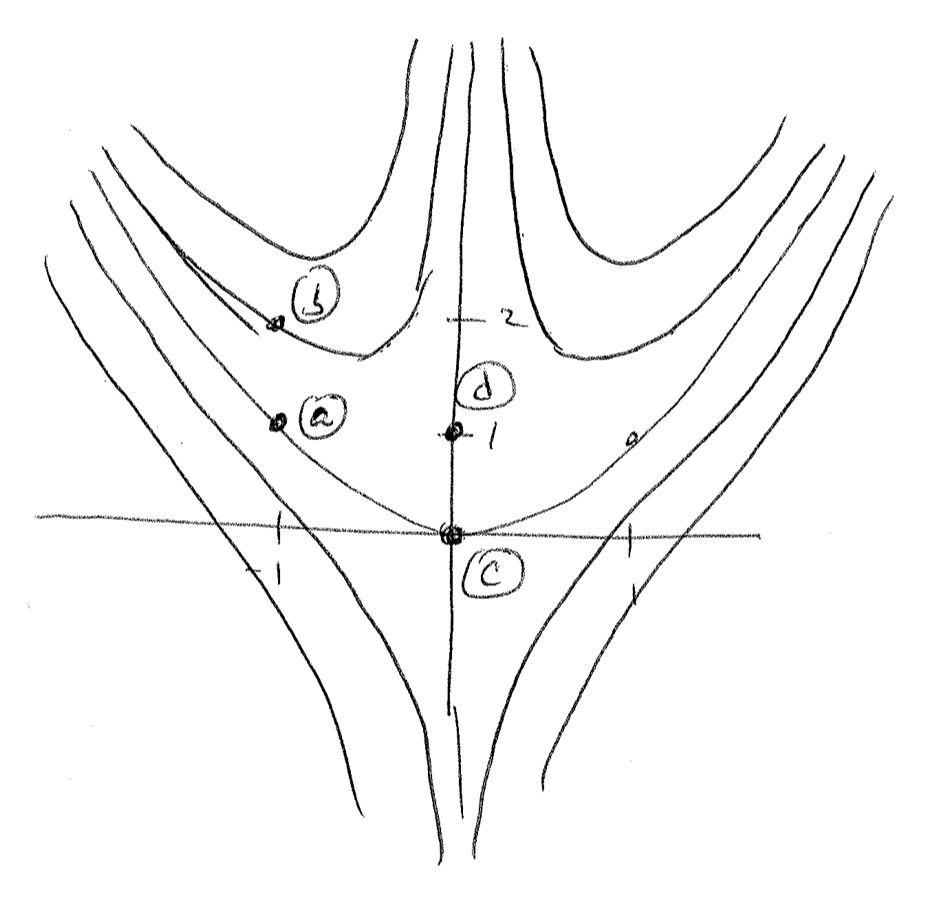
\includegraphics[width=10cm]{4-1}	
		\end{center}
		\begin{itemize}
			\item the domain of the IVP solution in \circled{a} is $(-\infty, \infty)$
			\item the domain of the IVP solution in \circled{b} is $(-\infty, 0)$
		\end{itemize}
		(This is only one piece of $ty(t) = t^2 + \frac{1}{t^2}$ the one that includes the point.)
		$\Rightarrow$ Solution to the IVP $ty' + 2y = 4t^2$, $y(0) = 1$ is
		\begin{equation*}
			\boxed{y(t) = t^2 + \frac{1}{t^2} \quad \text{ on } (-\infty, 0)}
		\end{equation*}
		\\
		\begin{center}
			\huge \underline{Careful here.}
		\end{center}
	\end{enumerate}
	
	 
\end{example-N}
\classheader{2018-06-19}
\subsection*{Modeling with First Order Equations}
This section deals with applications and the details of how to model a process to construct on ODE.\\
This, in general, is a difficult process and quite \underline{ad hoc}. Also it cannot be mastered in such a short time. Read this section.\\
\redhline\\
\subsection*{Non-Linear Equations}
In all examples shown, there has always been a solution. And with initial data, there has always been an \underline{unique solution.}
Is this always the case?\\
\begin{example-N}
	Solve $(y')^2 + 1 = 0$\\
	(Find a function whose derivative is -1?)
\end{example-N}
\begin{example-N}
	Solve $y' = \frac{3}{2} y^{\frac{1}{3}}$, $y(0)=0$\\
	Note that here that \circled{a} $y(t) \equiv 0$ solves this. But so does \circled{b} $y(t) = t^{\frac{3}{2}}$ \quad  \circled{c} $y(t) = -t^{\frac{3}{2}}$
	\begin{center}
	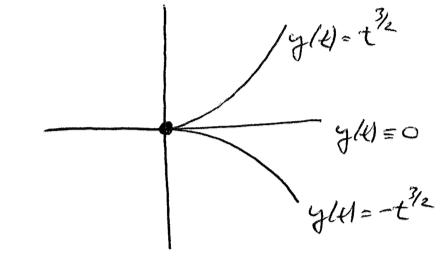
\includegraphics{5-1}		
	\end{center}

	Since all three of those distinct functions solve the IVP, we say solutions here (at $y(0)=0$) are \underline{NOT unique}!\\
\end{example-N}
\textbf{Question: } 16 Solutions to an ODE are not unique at a point $y(t_0) = y_0$, then 2 or more solutions that are distinct pass through the point. What does this say about the predictive power of your model?
\begin{center}
	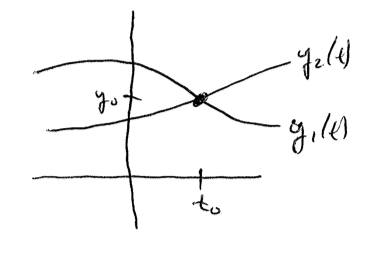
\includegraphics{5-2}
\end{center}
There are criteria for ensuring an IVP has solutions (sols. exist) and whether they are unique or not (unique is good!)\\\\
Let $(\star)\quad  y'(t) = f(t,y)$, $y(t_0) = y_0$ be an IVP
\begin{theorem-N}
	If $f(t,y)$ and $\dfrac{df}{dy}(t,y)$ are continuous in some rectangle $\alpha < t < \beta, \gamma < y < \delta$ containing $(t_0, y_0)$, then in some interval $t_0 - h < t < t_0 + h$ inside $\alpha < t < \beta$, there exists a unique solution $y(t)$ to $(\star)$\\
\end{theorem-N}

{\Large \underline{Many comments}}
\begin{enumerate}[label=\protect\circled{\alph*}]
	\item $f(t,y)$ and $\dfrac{df}{dy}(t,y)$ are functions of 2 variables. Continuity here is bigger than simply continuous in each variable while holding the other variable constant.
	\item $\dfrac{df}{dy}(t,y)$ is the derivative of $f$ with respect to $y$ while pretending $t$ is a constant.. It is called a \underline{partial derivative}.
	\item Geometrically, a solution passing though $(t_0, y_0)$ is an integral curve in the $ty-plane$.\\
	\begin{center}
		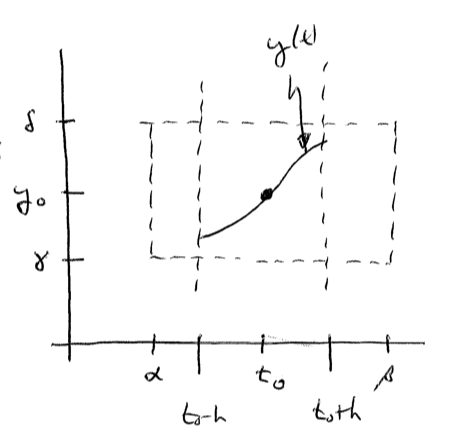
\includegraphics[scale=0.7]{5-3}		
	\end{center}
	\item $f(t,y)$ is continuous near $(t_0, y_0)$, then $y'(t)$ is continuous. But then by Calc I, $y(t)$ is differentiable. Hence solution \underline{exists} through $(t_0, y_0)$\\
	By Fundamental Theorem of Calculus, $y(t) = y(t_0) + \int_{t_0}^t f(s, y(s)) ds $.\\
	Since  $f(t,y)$ is continuous near $(t_0, y_0)$, then this integral will \underline{exist}. Note:
	\begin{equation*}
		y' = \dfrac{d}{dt}\bigg[y(t)\bigg] = \dfrac{d}{dt}\bigg[\int_{t_0}^t f(s, y(s)) ds\bigg] = f(t,y)
	\end{equation*}
	\item if $\dfrac{df}{dy}(t, y)$ is continuous near $(t_0, y_0)$, then solutions very nicely in the y-direction. This is enough to ensure solutions are \underline{unique}.\\
	$\Rightarrow$ Solution curves never touch or cross when uniquely defined. 
	\item \underline{Example: } Given $ty' + 2y = 4t^2$, if we place it in the form $y' = f(t,y)$, we set $y' = -\frac{2}{t}y + 4t$\\
	Here, as long as our initial data does not include $t_0 = 0$, solutions will exist\\ ($-\frac{2}{t}y + 4t$ is cont when $t\neq 0$) and unique when ($\dfrac{df}{dy}(t,y) = -\frac{2}{t}$ is continuous when $t \neq 0$)\\
	\textbf{Caution: } it may be possible for solutions to exist and/or be unique when $t=0$. But it is not assured!
	\begin{example-N}
		Given $y' = \frac{3}{2} y^{\frac{1}{3}}$, $f(t,y) = \frac{3}{2} y^{\frac{1}{3}}$.\\
		Here $f(t,y)$ is defined and continuous everywhere (and for all $t\in \mathbb{R}$, and $y \in \mathbb{R}$). Hence by Thm, \underline{solutions} are guaranteed to exist everywhere.\\
		But $\dfrac{df}{dy}(t,y) = \frac{1}{2}y^{-\frac{2}{3}}$ is not continuous along the $y=0$ line (in the $ty-plane$). Hence solutions exist for starting values like $y(t_0) = 0$, but \underline{may not be unique} (everywhere else they are unique!)
	\end{example-N}
	For any value $c \geq 0$, the curve $y(t) = 0, (t < c)$ and $(t-c)^{\frac{3}{2}} when, (t \geq c)$.\\
	Solve the IVP $y' = \frac{3}{2}y^{\frac{1}{3}}$, $y(0) = 0$
	\begin{center}
		\begin{tikzpicture}
			\begin{axis}
			[ymin = -1, ymax = 2,
			xmin = -1, xmax = 5,
			axis lines=center,
			axis on top=true,
			domain=0:4,
			xlabel={$x$},
    		ylabel={$y$},
    		samples=100]
    		\addplot[mark=none, draw=black, thin]{(x-0)^(3/2)} node [pos=0, below right, color=red]{$c=0$};
    		\addplot[mark=none, draw=black, thin]{(x-1)^(3/2)} node [pos=0, below right, color=red]{$c=1$};
    		\addplot[mark=none, draw=black, thin]{(x-2)^(3/2)} node [pos=0, below right, color=red]{$c=2$};
			\end{axis}
		\end{tikzpicture}
	\end{center}
	\item For linear ODE, existence and uniqueness is easier. In standard form,
	\begin{equation*}
		y' + p(t)y = q(t)
	\end{equation*}
	\begin{center}
		and in $y' = f(t,y)$ form
	\end{center}
	\begin{equation*}
		y' = \underbrace{-p(t)y + q(t)}_{f(t,y)}
	\end{equation*}
	\begin{theorem-N}
		As long as $p(t)$ and $q(t)$ are continuous at $t_0$, then solutions exist and are unique for $y' = -p(t)y + q(t)$, $y(t_0) = y_0$
	\end{theorem-N}
\end{enumerate}
\classheader{2018-06-20}
\underline{\Large New Question:} Suppose $y'=f(t,y)$, $f$ is \underline{ONLY} a function of y, but $\dfrac{1}{f(y)}$ is hard to integrate. How to study? $\boxed{\frac{1}{f(y)} \dfrac{dy}{dt} = 1}$\\
Here $y'=f(y)$ is called \underline{autonomous} ($t$ is not explicit in equation.)
\begin{example-N}
	\begin{equation*}
		\dot{x} = x^{\frac{2}{3}}, \quad y'=Ky, \quad \dfrac{dz}{dt} = z(1-z)
	\end{equation*}
	Then the solution curve will not depend on the starting time, only on the elapsed time. In the slope field, every vertical slice looks the same.\\
	Every horizontal slice is an isocline: a curve along which the slumps of the solution curves are the same.
	\begin{center}
	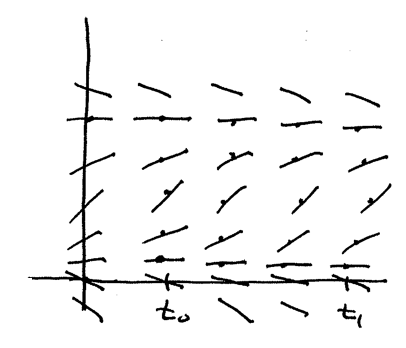
\includegraphics{6-1}\\
		Slopes along every vertical slice look like every other vertical slice. Slopes along every horizontal slice not very.
	\end{center}
\end{example-N}
\begin{enumerate}[label=\protect\circled{\Roman*}]
	\item Existence and uniqueness is determined by continuit of $f$ in $g$ and cont of $\dfrac{df}{dy}$ (not a partial here). 
	\item At any place, $y_0$ where $f(y_0) = 0$, then $y'(t) = 0$ and $y(t) = y_0$ is a \underline{constant solution}. Called an \underline{equilibrium solution}, its graph is horizontal and is an isocline.
		\begin{equation*}
			\dfrac{dz}{dt} = z(1-z). \quad \dfrac{dz}{dt} = 0 \quad \text{ when } z=0,1
		\end{equation*}
		\begin{equation*}
			\text{Hence } z(t) = 0 \text{ is a solution}
		\end{equation*}
		\begin{equation*}
			\text{Hence } z(t) = 1 \text{ is a solution}
		\end{equation*}
		\begin{center}
			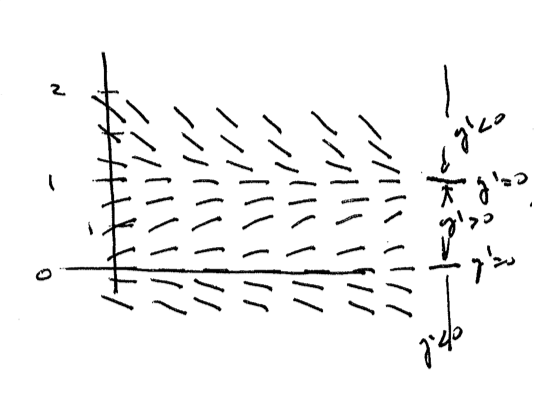
\includegraphics{6-2}
		\end{center}
	\item Outside of the equilibria solutions, of the "sign" of $\dfrac{dz}{dt}$ does not change, hence solutions stock between equilibria will have slopes always negative or always positive.\\
	{\small \textit{\underline{Note:} Without solving, you know pretty much everything. In fact, the slope field is too much information!}}
	\item One vertical slice through the slope field gives you all relevant info. For $z' = f(z) = z(1-z)$
	\begin{center}
	\begin{tikzpicture}
		\draw (-1,0) -- (2,0) ;
		\foreach \i in {0, 1}
			\draw (\i,0.1) circle + (0,-0.2) node[below] {$\i$};
		\foreach \i in {0, 1}
			\fill[red] (\i,0) circle (0.6 mm);
		\foreach \i in {-0.5, 1.5}
			\draw (\i,0.1) circle + (0,-0.1) node[below] {$<$};
		\foreach \i in {0.5}
			\draw (\i,0.1) circle + (0,-0.1) node[below] {$>$};
	\end{tikzpicture}
	\begin{center}
		Sign of $z'$ between equilibria
	\end{center}
	\end{center}
	This is called a \underline{phase line} (think of the y-axis slice in the ty-plane. It is a schematic that gives long term behavior of an autonomous 1st order ODE).
	\begin{example-N}
		Consider $z' = z(1-z), z(0) = \frac{3}{4}$.\\
		Without solving, we know by phase line that $\quad \lim_{t \to \infty } z(t) = 1 $
	\end{example-N}
	In fact, we know the long term behavior of all solutions.
	\begin{equation*}
	\lim_{t \to \infty}z(t) = 
		\begin{cases}
			-\infty & z(0) < 0\\
			0 & z(0) = 0\\
			1 & z(0) > 0
		\end{cases}
	\end{equation*}
	Without a slope field, one can simply graph $f(z)$.\\
	\begin{center}
	 Here on $(-\infty,0), \quad f(z) < 0, \quad z'<0$ for solutions.\\
	 Here on $(0,1), \quad f(z) > 0, \quad z'>0$ for solutions.\\
	   Here on $(1,\infty), \quad f(z) > 0, \quad z'<0$ for solutions.\\	
	\end{center}
	\begin{center}
	\begin{tikzpicture}
		\begin{axis}
		[xmin=-1, xmax=2,
		ymin=-1, ymax=0.6,
		axis lines=center,
		axis on top=true,
		domain=-1:4,
		xlabel={$x$},
    	ylabel={$y$},
    	samples=100]
		\addplot[mark=none, draw=black, thin]{x*(1-x)};
		\node[anchor=south] at (axis cs:0.5,0.3) {$f(z)$};
		\node[anchor=south] at (axis cs:1.5,0.3) {$z(1-z)$};
		\node[anchor=south, color=red] at (axis cs:-0.5,0.05) {$<$};
		\node[anchor=south, color=red] at (axis cs:0.5,0.05) {$>$};
		\node[anchor=south, color=red] at (axis cs:1.5,0.05) {$<$};
		\end{axis}
	\end{tikzpicture} 
	\end{center}
	\item We can use the the seaword derivative test to say more:\\
	$y' = f(y)$ for a solution, then $y'' = f'(y)y'$ helps to determine concavity of infection.\\
\end{enumerate}
\underline{Det:} For $y' = f(y)$, the set $\{y \in \mathbb{R} | f(y) = 0\}$ is the set of critical points for the ODE (equilibrium solutions).\\
Classification of critical points.
\begin{equation*}
	\text{let } y_{\star} \text{ be critical for } y'=f(y) \text{ and call } N_{\varepsilon}(y_{\star}) = \{ y \in \mathbb{R} | |y-y_{\star}| < \varepsilon  \} 
\end{equation*}
\begin{enumerate}[label=\protect\circled{\alph*}]
	\item If $\exists \varepsilon > 0 \text{ where } \forall y \in N_{\varepsilon}(y_{\varepsilon})$ and $\lim_{t \to \infty} y(t) = y_{\star} \Rightarrow y_{\star}$ is asymptotically stable.
	\item If $\exists \varepsilon > 0 \text{ where } \forall y \in N_{\varepsilon}(y_{\varepsilon})$ and $\lim_{t \to -\infty} y(t) = y_{\star} \Rightarrow y_{\star}$ is unstable.
	\item If stable on one side and unstable on other, semi-stable.\\
	\begin{center}
		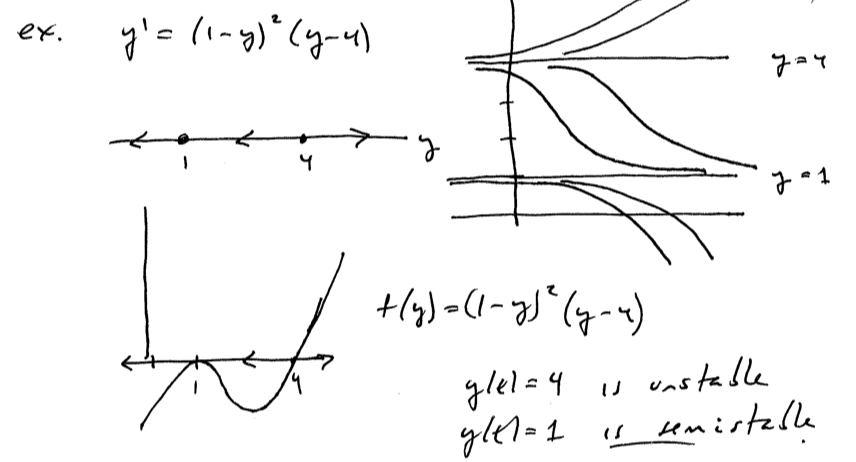
\includegraphics{6-3}		
	\end{center}	
\end{enumerate}
\classheader{2018-06-28}
\subsection*{Autonomous Equations and Population Dynamics}
{\large \underline{Equilibrium Solutions}}\\
At any place $y_0$ where $f(y_0) = 0$, then $y'(t) = 0$ here, and thus $y(t) = y_0$ is a constant solution (or equilibrium, or steady-state solution). Its graph is a horizontal line is an isocline.\\
\redhline
\begin{equation*}
	\dfrac{dz}{dt} = z(1-z)
\end{equation*}
\begin{center}
	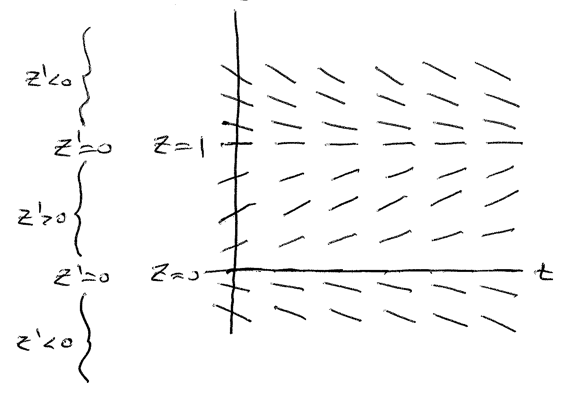
\includegraphics{7-1}
\end{center}
Here $Z(t) = 0$ and $z(t) = 1$ are both equilibrium solutions.\\
And between the equilibria, the \underline{sign} of $z'$ \underline{does not choose}. Hence solutions
\begin{enumerate}[label=\protect\circled{\Alph*}]
	\item are trapped between equilibria, and
	\item always travel in the same direction.
\end{enumerate}
In the example, we can say the following without solving:
\begin{enumerate}[label=\protect\circled{\Roman*}]
	\item Solutions exist and are unique everywhere ($f(z)$ and $f'(z)$ are polynomials)
	\item Equilibria only at $z=0$ and $z=1$.
	\item Any solution that pushes through $0 < Z_0 < 1$ will find toward the equilibria $z(t) = 1$.\\
		Any solution that starts at $Z_0 < 0$ will tend to $-\infty$\\
		Any solution that starts at $Z_0 > 1$ will tend to $z(t) = 1$\\ 
		Hence we can say
	\begin{equation*}
	\lim_{t \to \infty}z(t) = 
		\begin{cases}
			-\infty & Z_0 < 0\\
			0 & Z_0 = 0\\
			1 & Z_0 > 0
		\end{cases}
	\end{equation*}
\end{enumerate}
\redhline\\

{\large \underline{Phase Line}}\\
Any vertical slice through the slope field gives you all information about long term behavior solution:
\begin{center}
	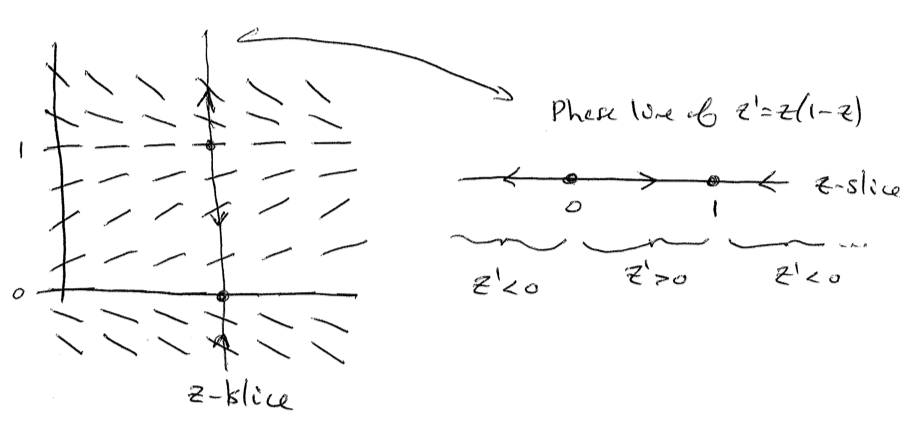
\includegraphics{7-2}
\end{center}
Here, the phase line is a schematic that determines all long term behavior of all autonomous $z'=f(z)$\\
Without a slope field still easy to see phase line: Graph $f(z)$: $z' = z(1-z) = f(z)$
\begin{center}
	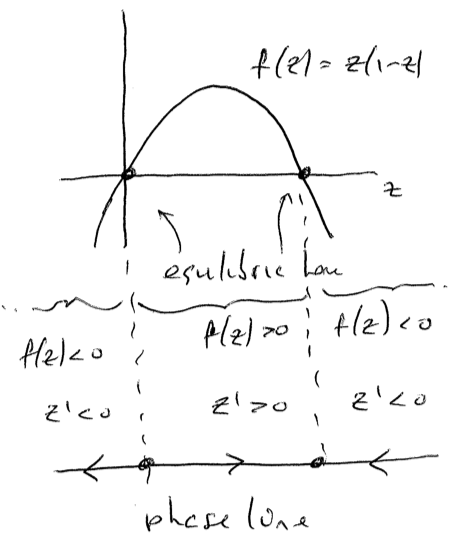
\includegraphics[scale=0.8]{7-3}
\end{center}
\begin{definition-N}
	For $y' = f(y)$, the set $\{ y \in \mathbb{R} \big| f(y) = 0\}$ is the set of \underline{critical points} for the ODE. (equilibrium solutions.)
\end{definition-N}
Critical points (equilibrium solutions) can be classified by how solutions behave around them:\\
Let $y_{\star}$ be a critical point for $y'=f(y)$ and let $N_{\varepsilon}(y_{\star}) = \{y \in  \mathbb{R} \big| |y - y_{\star} | < \varepsilon\}$ be an $\varepsilon-$neighborhood of $y_{\star}$.
\begin{enumerate}[label=\protect\circled{\alph*}]
	\item If there is a $\varepsilon > 0$ where for all $y \in N_{\varepsilon}(y_{\star})$
	\begin{equation*}
		\lim_{t \to \infty} y(t) = y_{\star} \Rightarrow \text{ is \underline{aymptotically stable}}
	\end{equation*}
	\item If there is an $\varepsilon > 0$ where for all $y \in N_{\varepsilon}(y_{\star})$
	\begin{equation*}
		\lim_{t \to -\infty} y(t) = y_{\star} \Rightarrow \text{ is \underline{unstable}}
	\end{equation*}
	\item If asymptotically stable on one side and unstable on the other, then $y_{\star}$ is semi-stable.
\end{enumerate}
\begin{example-N}
	$z' = z(1-z),$ Here critical points are $z = 0, 1$. And here $z(t) = 1$ is asymptotically stable and $z(t) = 0$ is unstable.
	\begin{center}
		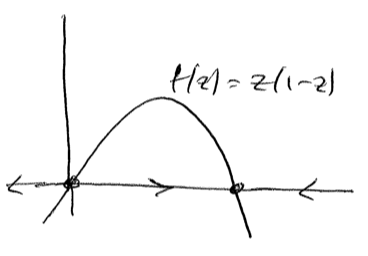
\includegraphics{7-4}
	\end{center}
\end{example-N}
\redhline\\
\begin{example-N}
	$y' = (1-y)^2 (y-4)$\\
	Here, critical points at $y=1,4$. The phase line is...
	\begin{center}
	\begin{tikzpicture}
		\draw (0,0) -- (6,0) ;
		\foreach \i in {1, 4}
			\draw (\i,0.1) circle + (0,-0.2) node[below] {$\i$};
		\foreach \i in {1, 4}
			\fill[red] (\i,0) circle (0.6 mm);
		\foreach \i in {0.5, 2.5}
			\draw (\i,0.1) circle + (0,-0.1) node[below, color=red] {$<$};
		\foreach \i in {5}
			\draw (\i,0.1) circle + (0,-0.1) node[below, color=red] {$>$};
	\end{tikzpicture}
	\\$y(t) = 4$ is unstable\\
	$y(t) = 1$ is semistable	\\
	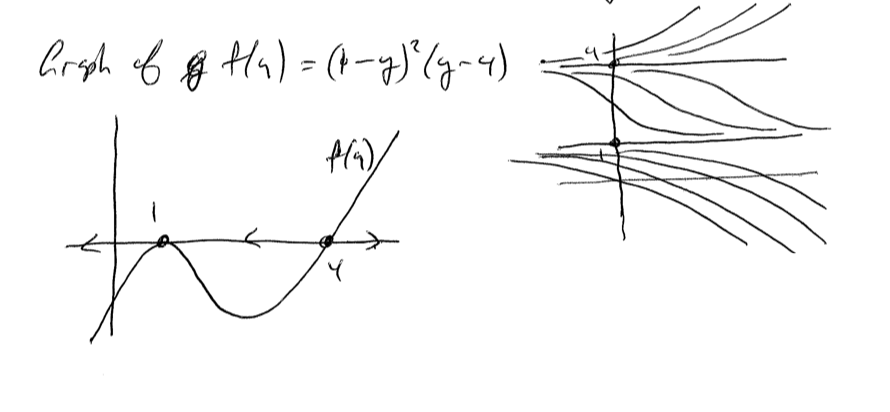
\includegraphics{7-5}
	\end{center}
	\begin{equation*}
		\lim_{t \to \infty} y(t) = 
		\begin{cases}
			\infty & y_0 > 4\\
			4 & y_0 = 4\\
			1 & 1 \leq y_0 < 4\\
			-\infty & y_0 < 1
		\end{cases}
	\end{equation*}
\end{example-N}
When graphing the $f(y)$ in $y'=f(y)$ and is constructing phrase lines, some patterns develop:\\
Let $y_{\star}$ be an equilibrium for $y'=f(y)$ (thus $f(y_{\star}) = 0$).\\
For $y$ "near" $y_0$, $y' = f(y) \cong \underbrace{ \cancelto{0}{f(y_{\star})} + f'(y_{\star}) (y-y_{\star})}_{\text{1st Taylor approx. to f(y) at } y_{\star}}$\\
{\large \textbf{Case 1:}} Suppose $f'(y_{\star}) > 0$
\begin{center}
	$\Rightarrow$ for $y>y_{\star}, \quad y'>0$
and $y < y_{\star}, \quad y' < 0$
\end{center}
\begin{center}
	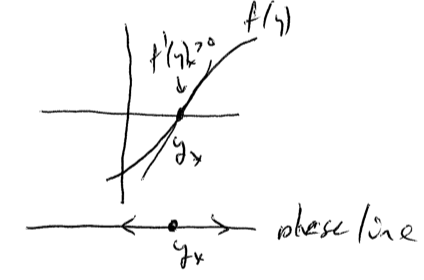
\includegraphics{7-6}
\end{center}
All nearby solutions move away $\Rightarrow y_{\star}$ is on unstable node or source\\
{\large \textbf{Case 2:}} Suppose for $f'(y_{\star}) < 0$
\begin{equation*}
	\Rightarrow \text{ for } y>y_{\star}, \quad y'<0 \text{ and } y < y_{\star}, \quad y' > 0
\end{equation*}
\begin{center}
	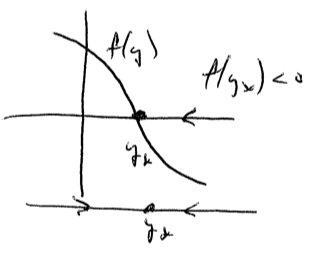
\includegraphics{7-7}
\end{center}
All nearby solutions converge to $y_{\star} \Rightarrow$ asymptotically stable on \underline{sink.}\\
{\large \textbf{Case 3:}} $f(y_{\star}) = 0$. Need more information.
\classheader{2018-06-30}
\subsection*{Bifurcations}
Consider the autonomous $y' = f(a,y)$ where "a" is a parameter. (an uniform constant). Equilibrium may depend on the value of a (in location \# and stability type).
\begin{example-N}
	$\dot{y} = ay - y^3 = y(a-y^2)$\\
	Here, for $a < 0$, and $a > 0$, the number of equilibria are different, also the type.
	\begin{center}
		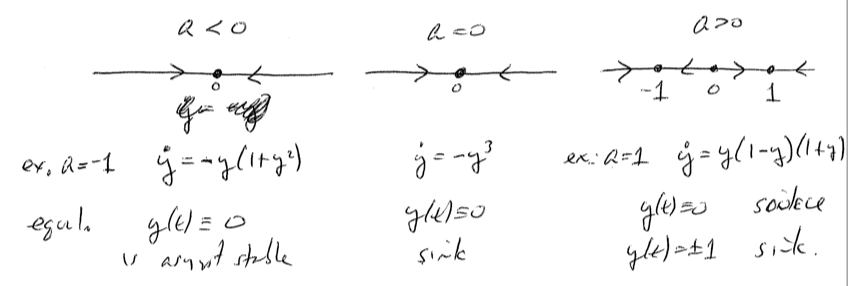
\includegraphics{7-8}
	\end{center}
\end{example-N}
We can study how $"a"$ affects equilibrium via a \underline{bifurcation diagram}
\begin{definition-N}
	A bifurcation diagram is graph of equilibrium (and stability) in relation to parameter value.
\end{definition-N} 
\redhline\\\\
{\large \underline{\textbf{Properties}}}
\begin{center}
	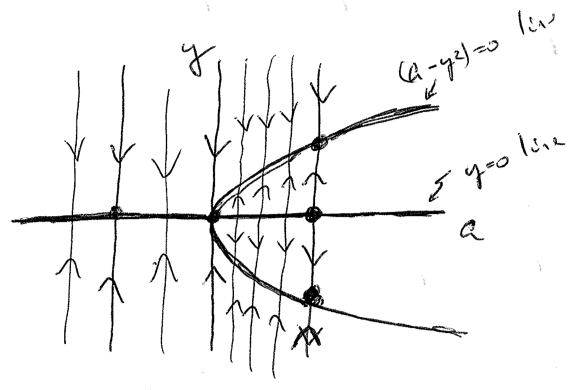
\includegraphics{7-9}
\end{center}
\begin{itemize}
	\item Each vertical slice is the phase line for a value of $a$.
	\item As $a$ varies, equilibrium trace out curves of fixed points. Found by solving $f(a,y) = 0$
	\item Curves of fixed points can be found by solving $f(a,y) = 0$\\
	$f(a,y) = y(a-y^2) = 0$, \quad when $\underbrace{y = 0}_{\text{a-axis}} \quad \underbrace{y^2 = a}_{\text{sideways parabola}} \Rightarrow y = \sqrt{a},$  $y = -\sqrt{a}$
	\item Here the only bifurcation value is $a = 0$
	\item Values of $a$ in which the stability and or \# of equilibria change are called \underline{bifurcation values} of $a$.
	\item \boxed{\text{These are rare!}} - stability cannot change outside of these!
\end{itemize}
{\Large \underline{Notes}}
\begin{enumerate}[label=\protect\circled{\Roman*}]
	\item Stable lines are used as phase lines to denote stability.
	\item Stability cannot change outside of bifurcation points, and cannot change far away.
	\item $a=0$ is called a pitchfork bifurcation for $\dot{y} = ay-y^3$.
\end{enumerate}
\begin{example-N}
	$\dot{y} = a-y^2$
	\begin{center}
		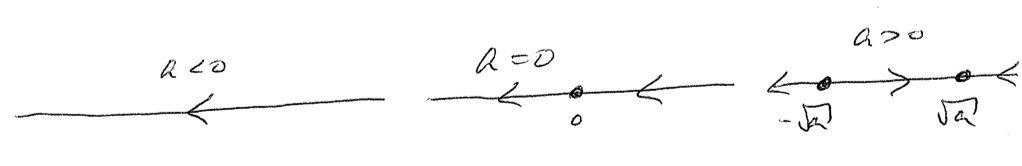
\includegraphics{7-10}
	\end{center}
	Lines of equil can only be $a-y^2 = 0 \Rightarrow a=y^2$ (sideways par).
	\begin{center}
		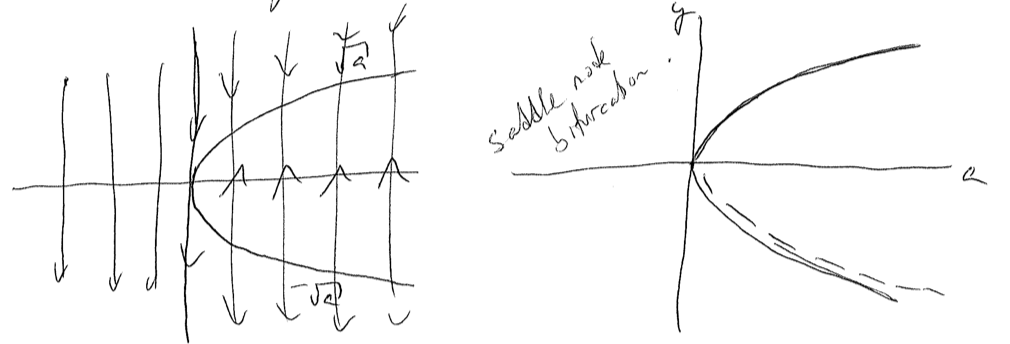
\includegraphics{7-11}
	\end{center}
\end{example-N}
\begin{example-N}
	$\dot{n} = (GN_0 - k)n - Gn^2$\\
	is an equation involving laser physics where $G, N_0, k$ are positive constants. $n(t)$ is the \# of photons along (always $n \geq 0$).\\
	Equilibrium solutions are $n(GN_0 - k - Gn) = 0$, where $n = 0$, $n = N_0 - \frac{k}{a}$.
	\begin{center}
	\underline{Bifurcation diagram.}\\
		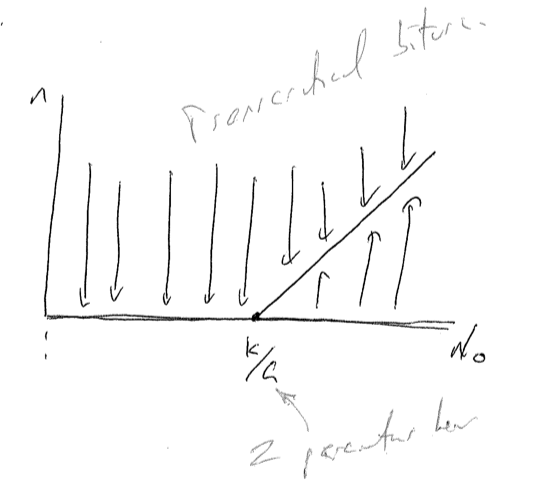
\includegraphics[scale=0.8]{7-12}
	\end{center}
\end{example-N}
\begin{enumerate}[label=\protect\circled{\Roman*}]
	\item when $N_0 < \frac{k}{a}$\\
	$\Rightarrow GN_0 - k < 0$\\
	$\Rightarrow \dot{n} < 0$\\
	$\Rightarrow n = 0$ is sink
	\item When $N_0 > \frac{k}{a}$, $GN_0 - k > 0$\\
	$\Rightarrow GN_0 - k - Gn$\\
	$N_0 - \frac{k}{a} - n > 0$ for small $n$.\\
	$\Rightarrow n = 0$ is a source\\
	if $N_0 - \frac{k}{a} - n < 0$ for $n > N_0 - \frac{k}{a}$\\
	$\Rightarrow N_0 - \frac{k}{a}$ is a sink
\end{enumerate}
\redhline\\
{\large \underline{Change track}} - Recall for any equation involving $x,y$,
\begin{itemize}
	\item We can bring all terms to one side of the equation and create an equivalent equation $\varphi (x, y) = 0$. For $\varphi (x,y)$ a function of 2 variables. Then the \underline{curve} in the xy-plane satisfying this equation is called the 0-level set of $\varphi$.
	\begin{example}
		$y^2 = 1-x^2$. We view this equation as the 0-level set of the function $\varphi(x,y) = x^2 + y^2 - 1 = 0$
	\end{example}
	\item We can view $y$ as a implicit function of $x$.\\
	In either case, the graph of the original equation (or the $\varphi(x,y) = 0$) is a curve in $xy$-plane that in general will not look like a function.\\
	We can calculate the tangent lines to this graph via differentiation in either interpretation.
	\begin{example}
		\begin{center}
			$x^2 + xy^2 = 4$, or $\varphi (x,y) = 0$, $\varphi (x,y) = x^2 + xy^2 - 4$
		\end{center}
		\begin{equation*}
			\text{\underline{Implicit diff}}\quad \dfrac{d}{dx}(x^2 +xy^2 = 4) \Rightarrow \underbrace{2x + y^2 +2xy \dfrac{dy}{dx}} = 0
		\end{equation*}	
		\begin{equation*}
			\text{\underline{Calc III}} \quad \dfrac{d \varphi}{dx}(x,y) = \dfrac{d \varphi}{dx} + \dfrac{d \varphi}{dy} \cdot \dfrac{dy}{dx} = \underbrace{\dfrac{d \varphi}{dx} + \dfrac{d \varphi}{dy} \cdot y'}_{(\star)}
		\end{equation*}
			{\tiny when we think of y as an implicit fraction of x.}
	\end{example}
\end{itemize}
\classheader{2018-07-08}
\subsection*{Exact Equations and Integrating Factors}
Suppose a first ODE has the form
\begin{equation*}
	\tcbhighmath[drop fuzzy shadow]{M(x,y) + N(x,y)y' = 0} \tag{$\ast$}
\end{equation*}
Then ($\star$) and ($\ast$) are the same under the condition thaht there exists a function.
\begin{align}
		\varphi(x,y), where \quad & \circled{1} \dfrac{d \varphi}{dx} (x,y) = M(x,y)\\
		& \circled{2} \dfrac{d \varphi}{dx} (x,y) = N(x,y)
\end{align}

\begin{equation*}
 	\text{So that} \quad \tikzmark{a}{M(x,y)} + \tikzmark{c}{N(x,y)}y' = 0 = \dfrac{d \varphi}{dx} = \tikzmark{b}{\dfrac{d \varphi}{dx}} + \tikzmark{d}{\dfrac{d \varphi}{dy}}y'
	\begin{tikzpicture}[overlay, remember picture]
	\draw[-, red](a) to [out=35,in=145](b);
	\draw[decorate] (a) to [out=35, in=145] (b);
	\draw[-, red](c) to [out=35, in=145](d);
	\draw[decorate] (c) to [out=35, in=145] (d);	
	\end{tikzpicture}
\end{equation*}
If this is the case, then the ODE $(\ast)$ can be rewritten as $\dfrac{d \varphi}{dx} = 0$, or $\varphi (x,y) = C$, a constant.
\begin{example}
	Notice that $2x + y^2 +2xyy' = 0$ is of the form $M(x,y) + N(x,y)y' = 0$ with
	\begin{align*}
		M(x,y) & = 2x + y^2\\
		N(x,y) & = 2xy
	\end{align*}
	But we also can see that the function $\varphi (x,y) = x^2 + xy^2$ has the partials.
	\begin{equation*}
		\dfrac{d \varphi}{dx} (x,y) = 2x + y^2 \quad \dfrac{d \varphi}{dy}(x,y) = 2xy
	\end{equation*}
	Hence $2x + y^2 + 2xyy' = 0$ can be written $\dfrac{d \varphi}{dx} = 0 = \dfrac{d}{dx}(x^2 + 2xy^2)$. If we assume that $y$ is an implicit function of $x$.\\
	here we can (assuming $y$ is an implicit function of x) integrate $\dfrac{d \varphi}{dx} (x,y) = 0$ w.r.t. $x$ to set
	\begin{equation*}
		\int \dfrac{d \varphi}{dx}(x,y) dx = \int 0 dx
	\end{equation*}
	\begin{equation*}
		\varphi (x,y) = x^2 + xy^2 = C
	\end{equation*}
	This is the implicit solution to
	\begin{equation*}
		2x + y^2 + 2xyy' = 0
	\end{equation*}
\end{example}
\redhline\\
\textbf{Question: } How do we know such a $\varphi (x,y)$ may exist and if so how to find it?\\\\
\underline{Calc III Thm} Let $\varphi (x,y)$ have continuous partial derivatives in some open region. Then
\begin{equation*}
	\dfrac{d}{dx} (\dfrac{d \varphi}{dx}) = \dfrac{d}{dy} (\dfrac{d \varphi}{dx}) \quad \textit{i.e. Mixed 2nd partials are equal.}
\end{equation*}
Now if we had the ODE
\begin{equation*}
	M(x,y) + N(x,y)\dfrac{dy}{dx} = 0
\end{equation*}
and knew there was a function $\varphi (x,y)$ when $\dfrac{d \varphi}{dx} = M$, $\dfrac{d \varphi}{dy} = N$. then the last criteria is
\begin{equation*}
	\dfrac{d}{dx}(\textbf{N}) = \dfrac{d}{dy}(\textbf{M}) \text{, or } \quad \tcbhighmath[drop fuzzy shadow]{N_{\textbf{X}} = M_{\textbf{Y}}}
\end{equation*}
\begin{definition-N}
	The ODE $M(x,y) + N(x,y)\dfrac{dy}{dx} = 0$ is called \underline{exact} on a region.
	\begin{equation*}
		R = \bigg\{ {(x,y) \in \mathbb{R}^2 \bigg| \begin{split}
			\alpha < x < \beta\\
			\gamma < y < \delta
		\end{split}} \bigg\} 
	\end{equation*}
	If \circled{1} $M, N, M_y, N_x$ are $C^0$ on $R$, and \circled{2} $M_y = N_x$ on $R$
\end{definition-N}
\begin{theorem-N}
	Let $M(x,y) + N(x,y)\dfrac{dy}{dx} = 0$ be exact o some open region $R$. Then $\exists$ a functions $\varphi(x,y)$ which is diff on $R$ where
	\begin{equation*}
		\circled{1} \dfrac{d \varphi}{dx} = M \quad \circled{2} \dfrac{d \varphi}{dy} = N
	\end{equation*} and $\varphi (x,y) = C$ is there general implicit solution to the ODE on $R$
\end{theorem-N}
\begin{example-N}
	Solve $(3x^2-2xy+2) + (6y^2 - x^2 + 3)y' = 0$, $y(1)=0$\\
	\underline{\large Strategy} First, we verify the exactness. Then we integrate to find the function whose level sets comprise solutions to the ODE.\\
	\underline{\large Solution} Here $M(x,y) = 3x^2 - 2xy + 2$, $N(x,y) = 6y^2 - x^2 + 3$ and since $M_y = \dfrac{dM}{dy} = -2x. = \dfrac{dN}{dx} = N_x$ the ODE is exact.\\
	And since $M, N, M_y, N_x$ are all $C^0$ on $\mathbb{R}^2$, by \underline{Thm} $\varphi (x,y)$ will exist near $(1,0) \in \mathbb{R}^2$. To find $\varphi (x,y)$, note that $\dfrac{d \varphi}{dx} = M$, $\dfrac{d \varphi}{dy} = N$.\\
	Integrate M \underline{wrt} x.
	\begin{equation*}
		\int M dx = \int \dfrac{d \varphi}{dx} dx = \int (3x^2 -2xy + 2)dx = x^3 -x^2y + 2x + \underbrace{h(y)}_{\text{why?}}
	\end{equation*}
	Hence $\varphi (x,y) = x^3 -x^2y + 2x + h(y)$ for some unknown function $h(y)$. To find $h(y)$, note that $\dfrac{d \varphi}{dy} = N$:
	\begin{align*}
		\dfrac{d \varphi}{dy}(x,y) & = \dfrac{d}{dx}(x^3 - x^2y + 2x + h(y))\\
		& = -x^2 + h'(y)\\
		& = N(x,y) = 6y^2 - x^2 + 3
	\end{align*}
	Hence $h'(y) = 6y^2 + 3$, or $h(y) = 2y^3 + 3y +$ \textit{constant}. Thus our general implicit solution is 
	\begin{equation*}
		\varphi(x,y) = x^3 - x^2y + 2x + 3y + 2y^2 = C
	\end{equation*}
	Our particular solution is $\varphi (1,0) = 1-0+2+0+0 = C$ or $c=3$, so $\varphi(x,y) = 3 = x^3 -x^y + 2x +3y +2y^3$. Determining a valid interval is difficult here. 
\end{example-N}
\begin{example-N}
	Solve $2x + y^2 + 2xyy'=0$, $y(1) = 1$\\
	\underline{\large Strategy} First, we verify the exactness. Then we integrate to find the function whose level sets comprise solutions to the ODE.\\
	\underline{\large Solution} Here $M(x,y) = 2x + y^2$, $N(x,y) = 2xy$ and since $M_y = \dfrac{dM}{dy} = 2y. = \dfrac{dN}{dx} = N_x$ the ODE is exact.\\
	And since $M, N, M_y, N_x$ are all $C^0$ on $\mathbb{R}^2$, by \underline{Thm} $\varphi (x,y)$ will exist near $(1,1) \in \mathbb{R}^2$. To find $\varphi (x,y)$, note that $\dfrac{d \varphi}{dx} = M$, $\dfrac{d \varphi}{dy} = N$.\\
	Integrate M \underline{wrt} x.
	\begin{equation*}
		\int M dx = \int \dfrac{d \varphi}{dx} dx = \int (2x + y^2)dx = x^2 + xy^2 + \underbrace{h(y)}_{\text{why?}}
	\end{equation*}
	Hence $\varphi (x,y) = x^2 + xy^2 + h(y)$ for some unknown function $h(y)$. To find $h(y)$, note that $\dfrac{d \varphi}{dy} = N$:
	\begin{align*}
		\dfrac{d \varphi}{dy}(x,y) & = \dfrac{d}{dy}(x^2 + xy^2 + h(y))\\
		& = 2xy + h'(y)\\
		& = N(x,y) = 2xy
	\end{align*}
	Hence $h'(y) = 0$, or $h(y) = $ \textit{constant}. Thus $\varphi (x,y) = x^2 + xy^2 + $ \textit{constant}, and $\varphi (x,y) = x^2 + xy^2 = C$ is our general implicit solution 
	The solution to $2x + y^2 + 2xyy' = 0$, $y(1) = 1$. $x^2 + xy^2 = 2$, variable on $x \in (0, \sqrt{2})$
\end{example-N}
{\large \textbf{\underline{Notes}}}
\begin{enumerate}[label=\protect\circled{\Roman*}]
	\item Sometimes, the ODE is in differential form:
	\begin{example}
		$(ye^{2xy} + x)dx + xe^{2xy}dy = 0$ is exact, since $M(x,y) = ye^{2xy} + x$, $N(x,y) = xe^{2xy}$ and 
		\begin{equation*}
			\textit{are equal}
			\begin{cases}
				M_y = e^{2xy} + 2xye^{2xy} \\
				M_x = e^{2xy} + 2xye^{2xy}
			\end{cases}
		\end{equation*}
	\end{example}
	\item Caution: Sometimes a \underline{non-exact} 1st order ODE can be made exact via an integration factor
		\begin{example}
		$dx + (\frac{x}{y} - \sin y)dy = 0$ is not exact $M_y = 0 \neq \frac{1}{y} = N_x$\\
		\begin{align*}
			y[dx + (\frac{x}{y} - & \sin y)dy  = 0]\\
			ydx + (x - y\sin y)dy & = 0 \text{ is exact since now }\\ M_y = 1 = \frac{d}{dx} [x - & y\sin y] = 1 = N_x
		\end{align*}
		\begin{center}
			We won't focus on this last technique.
		\end{center}
		\end{example}
\end{enumerate}

\classheader{2018-07-08}
I will relegate the discussion of Section of 2.8 to a worksheet posted. The theory can be deep (through very interesting). But the main takeaway is its usefulness in...
\begin{enumerate}[label=\protect\circled{\Roman*}]
	\item seeing where a first order ODE is "nice"
	\item Understanding the intricacies of the theory even at this early stage.
\end{enumerate}
\redhline
\section*{Second Order Linear Equations}
\subsection*{Homogeneous Equations with Constant Coefficients}
A general form of a 2nd order ODE is, for some function $f$
\begin{equation*}
	\tcbhighmath[drop fuzzy shadow]{y'' = f(t, y, y')} \tag{$\ast \ast$}
\end{equation*}
\begin{definition-N}
	A 2nd order ODE is called \underline{linear} if it can be written
	\begin{equation*}
		y'' + p(t)y' + q(t)y = g(t)
	\end{equation*}
	\begin{center}
		(so that $f(t, y, y') = g(t) - p(t)y' - q(t)$ in ($\ast$))\\
		($\ast \ast$) (actually $P(t)y'' + Q(t)y' + R(t)y = G(t)$...)
	\end{center}
	\underline{Notes}
	\begin{enumerate}[label=\protect\circled{\Roman*}]
		\item $f$ needs to be linear in both $y$ and $y'$
		\item If ODE is not linear, it is called non-linear.
	\end{enumerate}
\end{definition-N}
\begin{definition-N}
	If $g(t) \equiv 0$, then a linear ODE is called \underline{homogeneous}.
\end{definition-N}
\begin{definition-N}
	An IVP with a 2nd order ODE continuous 2 pieces of initial data, usually $y(t_0) = y_0$, $y'(t_0) = y_0'$
\end{definition-N}
\underline{Question:} Why?\\
In General, it is heard or impossible to solve a 2nd order ODE. Even linear is very difficult in general!\\
\redhline\\\\
One type that is solvable: Constant coefficients. Let ($\ast \ast$) here $P(t) \equiv a$, $Q(t) \equiv b$, $R(t) \equiv c$, and suppose $G(t) \equiv 0$ (homogenous).
\begin{equation*}
	\text{Then ODE is } \quad \tcbhighmath{ay'' + by' + cy = 0} \tag{$\star$}
\end{equation*}
\textbf{Q: } First think, what kinds of functions would possibly be solutions to their kind of ODE?
\begin{multicols}{2}
	\begin{itemize}
	\item Polynomials? Prove Functions?
	\item Trig functions?
	\item Exponentials?
	\item Logarithms?
	\end{itemize}
\end{multicols}
\begin{example-N}
	Suppose $a =1$, $b = 0$, $c = -1$, Then ($\ast \ast$) is $y'' - y = 0$, or $y'' = y$\\
	\underline{\large Solutions?}\\ Here $y(t) = e^t$ and $y(t) = e^{-t}$ both solve $y'' - y = 0$ How about $e^{t} + e^{-t}$? $2e^t - 3e^{-t}$? Here $y(t) = c_1e^t + c_2e^{-t}$ is a solution for any choice of $c_1, c_2 \in \mathbb{R}$\\
	What if IVP was $y''-y=0$, $y(0)=3$, $y(0) = 4$?
	\begin{equation*}
		y(0) = 3 = c_1 e^0 + c_2 e^{-0} = c_1 + c_2
	\end{equation*}
	\begin{equation*}
		\underbrace{y(0) = 4 = c_1 e^0 - c_2 e^{-0} = c_1 - c_2}_{\begin{split}c_1 = \frac{7}{2}\\ c_2 = -\frac{1}{2} \end{split} \quad \begin{cases}
			3 = c_1 + c_2\\ 4 = c_1 - c_2
		\end{cases}}
	\end{equation*}
	And the particular solution to IVP is 
	\begin{equation*}
		y(t) = \frac{7}{2}e^t - \frac{1}{2} e^{-t}
	\end{equation*}
\end{example-N}
\begin{example-N}
	$2y'' + 8y' -10y = 0$\\
	Here $y(t) = e^t$ and $y(t) = e^{-5t}$ both work! Check this... \underline{AND} so does $y(t) = c_1 e^t + c_2 e^{-5t}$. \underline{Is there a pattern?}
\end{example-N}
\redhline\\
For $ay'' + by' + cy = 0$, assume the solution is exponential (is this a good idea?) and looks like $y(t) = e^{\Gamma t}$, where $\Gamma$ is an unknown parameter.\\
Then substituting $y(t)$ and its derivatives into the ODE, we set
\begin{equation*}
	a\Gamma^2e^{\Gamma t} + b\Gamma e^{\Gamma t} + ce^{\Gamma t} = 0 \quad \textit{or} \quad a\Gamma^2 + b\Gamma + c = 0
\end{equation*}
Any valid values for $\Gamma$ must satisfy $\Gamma = \frac{-b \pm \sqrt{b^2 - 4ac}}{2a}$. \underline{Recognize this?}\\\\
For a 2nd order homogenous ODE with constant coefficients ($\star$) is called the \underline{characteristic equation}
\underline{\large \textbf{Important:}} When the two roots $\sqrt{1}$, $\sqrt{2}$ of the char. eqn. one \underline{real} and \underline{distinct}, then the general solution to the ODE is
\begin{equation*}
	\tcbhighmath[drop fuzzy shadow]{y(t) = c_1 e^{\Gamma_1 t} + c_2 e^{\Gamma_2 t}}
\end{equation*}
\begin{center}
	(we will need to make sure this is the case later)
\end{center}
\begin{example} $y''-y = 0$. Here $a = 1$, $b=0$, $c=1$, and characteristic equation is $\Gamma^2 - 1 = 0$, with roots $\Gamma = -1, 1$. General solution is 
\begin{equation*}
	y(t) = c_1e^t + c_2e^{-t}
\end{equation*}
\end{example}
\begin{example}
Characteristic equation is $2\Gamma^2 + 8\Gamma -10 = 0$ which factors to $(2\Gamma - 2)(\Gamma + 5) = 0$, so $\Gamma = 1, -5$.
\begin{equation*}
		y(t) = c_1e^t + c_2e^{-5t}	
\end{equation*}	
\end{example}


\classheader{2018-07-09}
Before talking about the cases where roots of the characteristic equation are the same or not real, lets return to the more general linear 2nd order homogenous ODE
\begin{equation*}
	y'' + p(t)y' + q(t)y = 0
\end{equation*}
To study this, form the operator (an operator is a function whose domain and range are functions).
\begin{equation*}
	L[\gamma] = \gamma'' + p(t)\gamma' + q(t) \gamma
\end{equation*}
This operator is defined for all $c^2$ functions $y(t)$ on an interval like $\alpha < t < \beta$, where $\alpha$ may be a number or $-\infty$, and $\beta$ may be a number or $\infty$.\\
\underline{\large Notes}
\begin{enumerate}[label=\protect\circled{\Roman*}]
	\item Can also write
	\begin{equation*}
		L = \dfrac{d^2}{dt^2} + p\dfrac{d}{dt} + q
	\end{equation*}
	\item An operator $L[\gamma]$ is \underline{linear} if $L[c_1\gamma_1 + c_2\gamma_2] = c_1L[\gamma_1] + c_2L[\gamma_2]$
	\begin{claim}
		$L[\gamma] = \gamma'' + p(t)\gamma' + q(t)$ is linear as an operator
	\end{claim}
	\begin{proof}
	\begin{align*}
		L[c_1\gamma_1 + c_2\gamma_2] & = \dfrac{d^2}{dt^2}\big[ c_1\gamma_1 + c_2\gamma_2\big] + p(t) \dfrac{d}{dt}\big[ c_1\gamma_1 + c_2\gamma_2 \big] +q(t)(c_1\gamma_1 + c_2\gamma_2)\\
		& = c_1\gamma_1'' + c_2\gamma_2'' + p(t)(c_1\gamma_1' + c_2\gamma_2') + q(t)(c_1\gamma_1'')\\
		& = c_1(\gamma_1'' + p(t)\gamma_1' + q(t)\gamma_1) + c2(\gamma_2'' + p(t)\gamma_2' + q(t)\gamma_2)\\
		& = c_1L[\gamma_1] + c_2L[\gamma_2]
	\end{align*}
	\end{proof}
\end{enumerate}
\underline{\large Fact:} The homogenous 2nd order linear ODE
\begin{equation*}
	y'' + p(t)y' + q(t)y = 0
\end{equation*}
is solved by \underline{any} function $y(t)$, where $L[y(t)] = 0$\\
\redhline
\begin{center}
	\Large \textbf{2 theorems on linear, $2^{nd}$ order ODE}
\end{center}
\redhline
\begin{enumerate}[label=\protect\circled{\Roman*}]
	\item Existence of Uniqueness
	\begin{theorem}
		The IVP $y'' + p(t)y' + q(t)y = g(t)$, $y(t_0) = y_0$, $y'(t_0) = y_0'$, where $p$, $q$, and $g$ are continuous on an open interval I containing $t_0$, has a unique solution $y(t)$ defined and twice differentiable on I.
	\end{theorem}
	\underline{\textbf{Note:}} Here, I can be taken to be the largest interval containing $t_0$, where $p$, $q$, and $g$ are all simultaneously continuous.
	\item Superposition
	\begin{theorem}
		If $y_1(t)$, $y_2(t)$ are 2 solutions to $L[y] = 0$, then so is $c_1\gamma_1 + c_2\gamma_2$ for all $c_1, c_2 \in \mathbb{R}$
	\end{theorem}
\end{enumerate}

\classheader{2018-07-09}
\subsection*{Solutions of Linear Homogenous Equations}
New Questions: If you found 2 solutions $y_1$, $y_2$ to $L[y] = 0$, do all solutions look like $c_1y_1 + c_2y_2$? Can there be others?\\
To study this, let's "solve" the IVP.
\begin{equation*}
	L[y] = 0, \quad y(t_0) = y_0, \quad y'(t_0) = y_0'
\end{equation*}
using the idea of a "general" solution
\begin{equation*}
	y(t) = c_1y_1(t) + c_2y_2(t)
\end{equation*}
\begin{align*}
	\overbrace{c_1y_1(t_0)}^{\text{real \#}} + \overbrace{c_2y_2(t_0)}^{\text{real \#}} = y_0\\
		c_1y_1'(t_0) + c_2y_2'(t_0) = y_0' \tag{$\star \star$}
\end{align*}
Solve the system for $c_1, c_2$ (2 eqns., 2 unknowns)\\
\redhline\\
\begin{equation*}
	\begin{split}
		c_1 = \dfrac{y_0 \cdot y_2'(t_0) - y_0' \cdot y_2(t_0)}{y_1(t_0) \cdot y_2'(t_0) - y_1'(t_0) \cdot y_2(t_0)}
	\end{split}
	\quad \quad \quad 
	\begin{split}
		c_2 = \dfrac{y_0 \cdot y_1'(t_0) - y_0' \cdot y_1(t_0)}{y_1(t_0) \cdot y_2'(t_0) - y_1'(t_0) \cdot y_2(t_0)}
	\end{split}
\end{equation*}
\textbf{Note:} Solutions to $(\star \star)$
\begin{center}
	1 solution \quad lines cross\\
	0 solutions \quad lines parallel\\
	$\infty$ solutions \quad lines the same
\end{center}
\textbf{Note:} the numerators are different for $c_1$, $c_2$ but the \underline{denominators} are \underline{the same!}\\
Rewrite the denominator as the determinant of a $2x2$ matrix whose entries are the coefficients of $(\star \star)$:
\begin{equation*}
	y_1(t_0) \cdot y_2'(t_0) - y_1'(t_0) \cdot y_2(t_0) = 
	\begin{vmatrix}
		y_1(t_0) & y_2(t_0) \\
		y_1'(t_0) & y_2' (t_0)
	\end{vmatrix}
\end{equation*}
This comes from writing $(\star \star)$ as a matrix equation:
\begin{equation*}
	\underbrace{\begin{bmatrix}
		y_1(t_0) & y_2(t_0) \\
		y_1'(t_0) & y_2' (t_0)
	\end{bmatrix}}_{A}
	\begin{bmatrix}
		c_1\\
		c_2
	\end{bmatrix}
	=
	\begin{bmatrix}
		y_0\\
		y_0'
	\end{bmatrix}
\end{equation*}
Given this matrix equation, if $\det A \neq 0$ there is a unique solution $(c_1, c_2)$\\
\redhline\\\\
In our case, in the 2 expressions for $c_1, c_2$
\begin{enumerate}[label=\protect\circled{\Roman*}]
	\item If denominator non-zero, then unique solution.
	\item if \underline{ONLY} denominator zero, then no solutions
	\item If both numerator, denominator zero, tons of solutions
\end{enumerate}
\begin{equation*}
	\text{Call} \quad W = W(y_1, y_2)(t_0) = 
	\begin{vmatrix}
		y_1(t_0) & y_2(t_0) \\
		y_1'(t_0) & y_2' (t_0)
	\end{vmatrix}
\end{equation*}
The \textbf{Wronskian determinant} of $y_1$, $y_2$ at $t_0$.
\begin{itemize}
	\item Tells you about the solutions to the IVP - $L[y] = 0$, $y(t_0) = y_0$, $y'(t_0) = y_0'$
\end{itemize}
\redhline
\begin{theorem-N}
	Suppose $y_1$, $y_2$ are 2 solutions to $l[y] = 0$ and at the initial values $y(t_0) = y_0$, $y_0'(t_0) = y_0'$ and $W(y_1, y_2)(t_0) \neq 0$
	\begin{center}
		$\Rightarrow \exists c_1, c_2 \in \mathbb{R}$ so that $y(t) = c_1 \cdot y_1(t) + c_2 \cdot y_2(t)$ solves the IVP.
	\end{center}
\end{theorem-N}
Note: This ensures that $y_1$ and $y_2$ are fundamentally "different" solutions (read: independent)
\begin{center}
	\textbf{Question:} What does this mean?
\end{center}
\begin{theorem-N}
	If $y_1$, $y_2$ both solve $L[y] = 0$, and if $\exists t_0$ where $W = W(y_1, y_2)(t_0)$, $\Rightarrow y(t) = c_1 y_1(t) + c_2 y_2(t)$ includes every solution!
\end{theorem-N}
\begin{proof}
	Let $\gamma$ be any solution to the IVP near $t_0$, where $W = W(y_1, y_2)(t_0)$. Then by \underline{theorem 1}, $c_1 y_1(t) + c_2 y_2(t)$ solves the IVP for some choice of $c_1, c_2 \in \mathbb{R}$. But by uniqueness $\gamma (t) = c_1 y_1(t) + c_2 y_2(t)$
\end{proof}
Here, given $L[y] = 0$, if you find any 2 solutions $y_1$, $y_2$ where Wronskian is somewhere non-zero, then $y(t) = c_1 y_1(t) + c_2 y_2(t)$ includes \underline{all} solutions on the entire \underline{interval} where Wronskin is non-non-zero. Called the general solution or the fundamental set of solutions to $L[y] = 0$\\
\begin{example-N}
	Suppose $y_1 = e^{\Gamma_1 t}$ and $y_2 = e^{\Gamma_2 t}$ both solve $L[y] = 0$. The Wronskin is
	\begin{equation*}
		W(y_1, y_2)(t) = 
		\begin{vmatrix}
			e^{\Gamma_1 t} & e^{\Gamma_2 t}\\
			\Gamma_1 e^{\Gamma_1 t} & \Gamma_2 e^{\Gamma_2 t}
		\end{vmatrix}
		 = (\Gamma_1 + \Gamma_2) e^{(\Gamma_1 + \Gamma_2)t}
	\end{equation*}
	Here, as long as $\Gamma_1 \neq \Gamma_2$, $W(y_1, y_2)(t) \neq 0$ anywhere on $\mathbb{R}$, and $y(t) = c_1 e^{\Gamma_1 t} + c_2 e^{\Gamma_2 t}$ is a fundamental set of solutions to $L[y'] = 0$
\end{example-N}
\redhline\\
\textbf{Example} $y_1 = \sin t$, $y_2 = \cos t$ and $W(y_1, y_2)(t) \equiv 1$\\
\textbf{Example} $y_1 = \sin t$, $y_2 = \cos (t - \frac{\pi}{2})$ and $W(y_1, y_2)(t) \equiv 0$\\
Where $W(y_1, y_2)(t) \neq 0$, we can say $y_1$, $y_2$ are linearly independent as functions.\\
\begin{definition}
	Two functions $f(x)$, $g(x)$ are called \underline{linearly dependent} \textbf{(LD)} on some open interval I if there exists 2 constants $k_1$, $k_2$ are not both 0, where
	\begin{equation*}
		k_1 f(x) + k_2 g(x) = 0
	\end{equation*}
	$\forall x \in I$. Otherwise called \underline{linearly independent} or \textbf{(LI)}
\end{definition}
\underline{Note:} If there exists one point $x \in I$ where 2 functions are \textbf{LI}, then the functions are \textbf{LI} on I.\\
\underline{Extra} The Wronskin only really depends on the ODE in a fundamental way:
\begin{theorem}
	Given any 2 solutions to $L[y] = 0$, where $p(t)$, $q(t)$ are continuous on an open interval $I$, then
	\begin{equation*}
		W(y_1, y_2) = ce^{-\int p(t) dt}
	\end{equation*}
	where $c$ depends on $y_1$, $y_2$ but not on $t$.
\end{theorem}
\underline{Notes}
\begin{enumerate}[label=\protect\circled{\Roman*}]
	\item If $y_1$, $y_2$ are \textbf{LD}, then $c=0$
	\item If $y_1$, $y_2$ are \textbf{LI}, then $W \neq 0$ on all of $I$
	\item Proof is quire interesting!
	\item LI and non Wronskin are the same thing for ODEs.
\end{enumerate}
\begin{proof}
	Since $y_1$, $y_2$ solve the ODE
	\begin{enumerate}[label=\protect\circled{\alph*}]
		\setlength\itemindent{25pt} \item $y_1'' + p(t)y_1' + q(t)y_1 = 0$
		\item $y_2'' + p(t)y_2' + q(t)y_2 = 0$
	\end{enumerate}
	Must \circled{a} by $-y_2$ and \circled{b} by $y_1$ and add (eliminating $q(t)$)
	\begin{equation*}
		\underbrace{\underbrace{y_1 y_2'' - y_2 y_1''}_{W'(y_1, y_2)} + p(t) \underbrace{y_1 y_2' - y_2 y_1'}_{W(y_1, y_2)}}_{W' + p(t)W = 0} = 0
	\end{equation*}
	is a 1st order ODE in the Wronskin $\det$ as a function of $t$. By separation of variables:
	\begin{align*}
		\frac{W'}{W} = -p(t) & \Rightarrow \ln |W| = - \int p(t) \det K\\
		& \Rightarrow W = ce^{-\int p(t) dt}
	\end{align*}
	Eitehr $W = 0$ on all of $I$ or $W \neq 0$ on all of $I$
\end{proof}

\classheader{2018-07-09}
\subsection*{Complex Roots of the Characteristic Equation}
Back to the constant coefficients case:
\begin{equation*}
	ay'' + by= + cy = 0 \tag{$\star$}
\end{equation*}
Let $a = 1 = c$, $b = 0$. Here $y'' + y = 0$ has characteristic equation $\Gamma^2 + 1 = 0$ (no real solutions).\\
But we know $y_1(t) = \cos t$, $y_2(t) = \sin t$. Solve $y'' + y = 0$
\begin{equation*}
	\tcbhighmath[drop fuzzy shadow]{y(t) = c_1 \cos t + c_2 \sin t}
\end{equation*}
\redhline
\begin{center}
	\textbf{Question:} How can we get that from the characteristic equation?
\end{center}
\redhline\\
First, $r^2 + 1 = 0$ does have 2 solutions: $r = \pm i$\\
Sticking to the exponential there, $y_1(t) = e^{it}$ and $y_2(t) = e^{-it}$ are the two solutions.\\\\
\textbf{Recall Euler's Formula}
\begin{equation*}
	e^{(a + ib)t} = e^{at}(\cos bt + i \sin bt)
\end{equation*}
\redhline
\begin{center}
	\textbf{Question:} Can we construct real solutions from there?
\end{center}
Suppose an ODE has characteristics equation.
\begin{equation*}
	a\Gamma^2 + b \Gamma + c = 0, \quad \Gamma = \frac{-b \pm \sqrt{b^2 - 4ac}}{2a} = \lambda \pm \mu i, \quad \mu \neq 0 
\end{equation*}
Writing 2 exponential solutions.
\begin{equation*}
	\begin{split}
			y_1(t) & = e^{(\lambda + \mu i)t}\\
			& = e^{\lambda t}(\cos \mu t + i\sin \mu t)
	\end{split}
	\quad \quad \quad 
	\begin{split}
			y_1(t) & = e^{(\lambda - \mu i)t}\\
			& = e^{\lambda t}(\cos \mu t - i\sin \mu t)
	\end{split}
\end{equation*}
We see they are not real. But real ODE must be real solutions!\\
The \underline{superposition}, any linear combination of $y_1$, $y_2$ is also a solution:
\begin{align*}
	\text{Hence } \quad \frac{1}{2}(y_1(t) + y_2(t))  & = \frac{1}{2} (e^{\lambda t} \cos \mu t + i \sin \mu t) + e^{\lambda t} \cos \mu t + i \sin \mu t\\
	& = e^{\lambda t} \cos \mu t \quad \text{is a solution}
\end{align*}
\begin{align*}
	\text{Hence } \quad \frac{1}{2i}(y_1(t) - y_2(t))  & = \frac{1}{2i} (e^{\lambda t} \cos \mu t + i \sin \mu t) - e^{\lambda t} \cos \mu t + i \sin \mu t\\ & = e^{\lambda t} \sin \mu t \quad \text{is a solution}
\end{align*}
lets call then $u(t) = e^{\lambda t} \cos \mu t$, \quad $v(t)=e^{\lambda t} \sin \mu t$\\
There a 2 real solutions (the real and imaginary parts of the original operator solutions.)\\
\underline{And} since $W(u,v) = $ calculate this $= \mu e^{2 \lambda t} \neq 0$ anywhere as long as $\mu \neq 0$, the fund set of solutions is.
\begin{align*}
	y(t) & = c_1 e^{\lambda t} \cos \mu t + c_2 e^{\lambda t} \sin \mu t \\
	& = e^{\lambda t}(c_1 \cos \mu t + c_2 \sin \mu t)
\end{align*}
\begin{example-N}
	$y'' + y = 0$. Roots of $\Gamma^2 + 1 = 0$ are $\Gamma = \pm i$. Here $\lambda = 0$, $\mu = 1$.
	\begin{equation*}
		y(t) = e^{0t}(c_1 \cos 1t + c_2 \sin 1t) = \boxed{c_1 \cos t + c_2 \sin t}
	\end{equation*}
\end{example-N}
\begin{example-N}
	Solve the IVP $y'' + 4y' + 13y = 0$, $y(0) = 2$, $y'(0) = 7$\\
	\underline{Solution}: The characteristic equation is $\Gamma^2 + 4\Gamma + 13 = 0$, and $\Gamma. = \frac{-4 \pm \sqrt{16 - 52}}{2} = -2 \pm 3i$\\\\
	Here, find set of solutions is 
	\begin{equation*}
		y(t) = e^{-2t}(c_1 \cos 3t + c_2 \sin 3t)
	\end{equation*}
	For a particular solution
	\begin{align*}
		y(0) & = e^{-2(0)}(c_1 \cos 3(0) + c_2 \sin 3(0)) = \boxed{2 = c_1}\\
		y'(0) & = -2e^{-2t}(c_1 \cos 3t + c_2 \sin 3t) + e^{-2t}(-6 \sin 3t + 3c_2 cos 3t) \Bigg|_{t=0} \\
		& = -4 + 3c_2 = 7 \quad c_2 = \frac{11}{3}
	\end{align*}
	\begin{equation*}
		\boxed{y(t) = e^{-2t}(2 \cos 3t + \frac{11}{3} \sin 3t)}
	\end{equation*}
\end{example-N}
\redhline\\
\underline{\textbf{Facts}} Given $ay'' + by' + cy = 0$ and its characteristic equation $a\Gamma^2 + b\Gamma + c = 0$ with roots $\Gamma_1$, $\Gamma_2$:
\begin{enumerate}[label=\protect\circled{\Roman*}]
	\item $\Gamma_1 \neq \Gamma_2$, where real roots
	\begin{equation*}
		y(t) = c_1 e^{\Gamma_1 t} + c_2 e^{\Gamma_2 t} \tag{real roots}
	\end{equation*}
	\item $\Gamma_1 = \lambda + i\mu \neq \lambda - i\mu = \Gamma_2$, complex roots
	\begin{equation*}
		y(t) = e^{\lambda t} (c_1 \cos \mu t + c_2 \sin \mu t) \tag{complex roots}
	\end{equation*}
	\item $\Gamma_1 = \Gamma_2 = \Gamma$, equal roots
	\begin{equation*}
		y(t) = c_1 e^{\Gamma t} + c_2 e^{\Gamma t} = (c_1 + c_2)e^{\Gamma t} = K e^{\Gamma t} \tag{equal roots}
	\end{equation*}
	Is only 1 solution. We will need another linear independent one to construct a fund set of solutions.
\end{enumerate}
\classheader{2018-07-10}
\subsection*{Repeated Roots; Reduction of Order}
\underline{Reduction of order} - Using one solution to an nth-order ODE to create on $(n-1)$th order ODE.\\
Suppose ($\star$) $y'' + p(t)y' + q(t)y = 0$ has $y_1(t)$ as a non-zero solution. If you can find an independent second solution, you are done.\\
\underline{Guess:} Assume second solution has the form $y_2(t) = v(t)y_1(t)$ for some function $v(t)$.\\
Why? you will see.\\
\underline{Good: } Try to solve the $v(t)$.\\
Now if $y_2(t)$ solves the ODE, then
\begin{align*}
	y_2'(t) = \dfrac{d}{dt}[v(t)y_1(t)] = v'(t)y_1(t) + v(t)y_1(t)\\
	y_2''(t) = v''(t)y_1(t) + \underbrace{v'(t)y_1'(t) + v'(t)y_1'(t)}_{2v'(t)y_1'(t)} + v(t)y_1''(t)
\end{align*}
Substitute this back into the original ODE: 
\begin{equation*}
	\underbrace{(v''y_1 + 2v'y_1' + vy'')}_{y_2''} + p\underbrace{(v'y_1 + vy_1')}_{y_2'} + q \underbrace{vy_1}_{y_2} = 0
\end{equation*}
Recall in terms of $v$ and derivatives:
\begin{equation*}
	y_1v'' + (2y_1' + py_1)v' + \underbrace{(y_1'' + py_1' + qy_1)}_{=0}v = 0 \tag{we guess $y_2 = vy_1$}
\end{equation*}
We left with:
\begin{equation*}
	y_1v'' + (2y_1' + py)v' = 0 \tag{$\star$}
\end{equation*}
This is a 2nd order ODE in $v(t)$. But this is a 1st order ODE in $v'(t)$!!
\begin{center}
	\boxed{\text{\Large Solve for $v'(t)$. Then integrate to set $v(t)$.}}
\end{center}
{\large \underline{Notes:}}
\begin{enumerate}[label=\protect\circled{\Roman*}]
	\item Thinking of ($\star$) is a 1st order ODE in $v'(t)$ is called \underline{reducing the order}.
	\item If the coefficient of $v(t)$ weren't $0$, then we cannot do this! Since the lowest order derivative is $v'$, we can.
	\item For independence,
	\begin{align*}
		W(y_1, vy_1) & = 
		\begin{vmatrix}
		y_1 & vy_1 \\
		y_1' & v'y_1 + vy_1' \\	
		\end{vmatrix}\\
		& = v_1y_1^2 + \underbrace{vy_1y_1' - vy_1y_1'}_{\text{cancel}} = v_1y_1^2
	\end{align*}
\end{enumerate}
As long as $v_1' \neq 0$, (so $v_1(t)$ is not a constant) $y_2 = v_1y_1$ will be independent of $y$.
\begin{example-N}
	$y_1(t) = \frac{1}{t}$ solves $t^2y'' + cty' + y = 0$ on the interval $t > 0$. Find the set of fundamental solutions.\\
	\redhline
	\begin{center}
		\underline{Strategy:} Use reduction of order.
	\end{center}
	\redhline\\
	\underline{Solution:} Both $p(t) = \frac{3}{t}$, $q(t) = \frac{1}{t^2}$, are $C^0$ on $(0, \infty)$. Assume $y_2(t) = v(t)y_1(t) = \frac{v(t)}{t}$\\
	Then $v(t)$ solves
	\begin{align*}
		y_1v'' + (2y_1' + py_1)v' = 0 \text{, or }\\
		\frac{1}{t}v'' + (2(-\frac{1}{t^2}) + (\frac{3}{t})(\frac{1}{t}))v' = 0\text{, or }\\
		\frac{v''}{t} + \frac{v'}{t^2} = 0 \Rightarrow tv'' + v = \dfrac{d}{dt}[tv'] = 0 
	\end{align*}
	which implies $tv' = c$, a constant, or $v'(t) = \frac{c}{t}$, or $v(t) = c_1\ln t + c_2$ on $t=0$
	\begin{equation*}
		\text{Hence} \quad \quad y_2(t) = \frac{v(t)}{t} = \frac{c_1 \ln t + c_2}{t}
	\end{equation*}
\end{example-N} 
{\large \underline{Questions to ask}}
\begin{enumerate}[label=\protect\circled{\Roman*}]
	\item Does $y_2(t)$ actually solve the original ODE?
	\begin{equation*}
		y_2(t) = \frac{c_1 \ln t + c_2}{t}, \quad y_2'(t) = c_1 \bigg( \frac{1 - \ln t}{t^2} \bigg) - \frac{c_2}{t^2}, \quad y_2''(t) = c_1 \bigg(\frac{2 \ln t - 3}{t^3} \bigg) + \frac{2c_2}{t^3}
	\end{equation*}
	Here
	\begin{align*}
		t^2y'' + 3ty' + y = 0 = t\bigg(c_1\bigg(\frac{2 \ln t - 3}{t^3}\bigg) - \frac{2c_2}{t^3}\bigg) + 3t\bigg(c_1  \big(\frac{1 - \ln t}{t^2} - \frac{c_2}{t^2}\big)\bigg) + \frac{c_1 \ln t + c_2}{t}\\
		= c_1\bigg(\frac{2 \ln t - 3}{t} \bigg) - \frac{2c_2}{t} + 3c_1(\frac{1 - \ln t}{t}) - \frac{3c_2}{t} + c_1 \frac{\ln t}{t} + \frac{c_2}{t} = 0 
	\end{align*}
	\item Notice that $y_1 = \frac{1}{t}$ appears as a summed in $y_2 = c_1 \frac{\ln t}{t} + \frac{c_2}{t}$. By Superposition, it is not really needed. Check independence of $y_1$, $y_2$.
\end{enumerate}
Hence fundamental set of solutions is 
\begin{align*}
	y(t) & = \text{(constant)}y_1 + \text{(constant)}y_2\\
	& = \text{(constant)} \frac{1}{t} + \text{(constant)} \bigg(c_1 \frac{\ln t}{t} + c_2 \big(\frac{1}{t}\big)\bigg)
\end{align*}
Combine constants to get
\begin{equation*}
	\tcbhighmath[drop fuzzy shadow]{y(t) = \frac{K_1}{t} + K_2 \frac{\ln t}{t}} \quad \quad \text{as the general solution.}
\end{equation*}
\underline{Application} Given $ay'' + by' + cy = 0$.\\
Suppose characteristic equation has only 1 real solution.
\begin{equation*}
	\text{Then} \quad \Gamma = \frac{-b \pm \sqrt{b^2 - 4ac}}{2a} = \frac{-b}{2a}
\end{equation*}
Here $y_1(t) = e^{-\frac{b}{2a}t}$ solves the ODE, but this is the only exponential function that does. To find another function \underline{reduce the order:}\\\\
Assume $y_2 = v(t) e^{-\frac{b}{2a}t}$, where $v(t)$ solves
\begin{equation*}
	v''y + (2y_1' + py_1)v_1 = 0, \quad \text{or} \quad e^{-\frac{b}{2a}t}v'' + \underbrace{\bigg( 2(\frac{b}{2a}t e^{-\frac{b}{2a}t}) + \frac{b}{a} \frac{b}{2a}t\bigg)}_{0}v' = 0 
\end{equation*}
\begin{equation*}
	\Rightarrow e^{-\frac{b}{2a}t}v'' = 0 \Rightarrow v'' = 0 \Rightarrow v(t) = K_1 t + K_2
\end{equation*}
\begin{center}
	So $y_2(t) = (K_1 t + K_2) e^{-\frac{b}{2a}t}$
\end{center}
\begin{exercise}
Calculate $W(y_1, y_2)$ here!\\
Hence  $y_1(t), y_2(t)$ form a fundamental set of solutions,
\begin{equation*}
	y(t) = \text{(constant)} e^{-\frac{b}{2a}t} + \text{(constant)}(K_1 + K_2) e^{-\frac{b}{2a}t} 
\end{equation*}
\begin{equation*}
	\tcbhighmath[drop fuzzy shadow]{y(t) = C_1 e^{-\frac{b}{2a}t} + C_2 e^{-\frac{b}{2a}t}}
\end{equation*}
\end{exercise}
\redhline
\begin{example-N}
	Solve $25y'' - 20y' + 4y = 0, \quad y(0) = 5, y'(0) = \frac{3}{2}$\\
	\underline{Solution}: Here discriminant $b^2 - 4ac = 400 - 400 = 0$\\
	\begin{center}
	Hence $\Gamma_1 = \Gamma_2 = \Gamma = -\frac{b}{2a} = \frac{2}{5}$\\
	Hence fundamental set of solutions is:
	\begin{equation*}
		y(t) = C_1 e^{\frac{2}{5}t} + C_2 e^{\frac{2}{5}t}
	\end{equation*}
	As for the particular solution:
	\begin{equation*}
		y(0) = C_1 e^0 + C_2 e^0 = 5 = C_1
	\end{equation*}
	So $y(t) = C_1 e^{\frac{2}{5}t} + C_2 e^{\frac{2}{5}t}$\\
	And $y(t) = 5 (\frac{2}{5}) e^{\frac{2}{5}t} + C_2 e^{\frac{2}{5}t} + \frac{2C_2}{5}t e^{\frac{2}{5}t} \Bigg|_{t = 0}$\\
	$ = 2 + C_2 = \frac{3}{2} \Rightarrow C_2 = \frac{-1}{2}$
	\end{center}
	\begin{equation*}
		\text{Solution is} \quad \tcbhighmath[drop fuzzy shadow]{y(t) = 5 e^{\frac{2}{5}t} - \frac{t}{2} e^{\frac{2}{5}t}}
	\end{equation*}
\end{example-N}


\classheader{2018-08-14}
\subsection*{Nonhomogeneous Equations; Method of Undetermined Coefficients}
Let's go back to the original linear
\begin{equation*}
	L[y] = y'' + p(t)y' + q(t) = g(t) \tag{+}
\end{equation*}
where $p$, $q$, and $g$ are continuous on some $I$ and $g(t) \neq 0$ (The non-homogenous case)\\
{\textbf{Note:}} $(+)$ is linear, but superposition \underline{only} holds for the LHS!
\begin{theorem}
	Suppose $\Ylines_1 (t)$ solves $L[y] = g_1(t)$ and $\Ylines_2 (t)$ solves $L[y] = g_2(t)$
\end{theorem}
\begin{proof}
	$L[\Ylines_1 + \Ylines_2] = L[\Ylines_1] + L[\Ylines_2] = g_1(t) + g_2(t)$
\end{proof}
\begin{corollary}
	Suppose $\Ylines_1 (t)$ and $\Ylines_2 (t)$ both solve $L[y] = g(t)$. Then $\Ylines_2 (t) - \Ylines_1(t)$ solve $L[y] = 0$.
\end{corollary}
Let $L[y] = g(t)$ be non-homogenous, and $\Ylines_1(t)$ and $\Ylines_2(t)$ be 2 solutions.\\
Let $c_1y_1(t) + c_2y_2(t)$ be a fundamental set of solutions to the homogenous $L[y] = 0$.\\\\
Since $\Ylines_2 (t) - \Ylines_1(t)$ solves $L[y] = 0$ also, we set:
\begin{enumerate}[label=\protect\circled{\Roman*}]
	\item $\Ylines_2 (t) - \Ylines_1(t) = c_1y_1(t) + c_2y_2(t)$ \textit{for some values of $c_1$, $c_2$} 
	\item $\underbrace{\Ylines_2}_{\text{any other soln. to } L[y] = g(t) } = \underbrace{c_1y_1(t) + c_2y_2(t)}_{\text{fund. set of solns to L[y] = 0}} + \underbrace{\Ylines_1(t)}_{\text{a soln. to } L[y] = g(t)}$ 
\end{enumerate}
We use this to set
\begin{theorem}
	The general solution to $L[y] = g(t)$ is $y(t) = c_1y_1(t) + c_2y_2(t) + \Ylines(t)$\\
	where $y_1$, $y_2$ form a fund. set of solns. to $L[y] = 0$, and $\Ylines(t)$ is \underline{ANY} particular solution to $L[y] = g(t)$
\end{theorem}
This gives us a method for solving $L[y] = g(t)$:
\begin{enumerate}[label=\protect\circled{\Roman*}]
	\item First, solve $L[y] = 0$
	\item Find any soln to $L[y] = g(t)$
	\item Put them together to get general solution
\end{enumerate}
So the new question appears: Find a particular solution to $L[y] = g(t)$. 
\underline{In general, this is hard}, But there are ways. [Assume the form of a solution and solve.]
\subsubsection*{Undetermined coefficients}
Say ODE part has:
\begin{enumerate}[label=\protect\circled{\Roman*}]
	\item homogenous part with constant coefficients
	\item $g(t)$ is a sum of products of
	\begin{enumerate}[label=\protect\circled{\alph*}]
		\item exponent
		\item sins and cosines
		\item polynomials
	\end{enumerate}
\end{enumerate}
Then you can assume the solution is also of a similar type. Write it out with some unknown coefficients, sub in and solve for the coefficients.
\begin{example-N}
	Solve $y'' - 2y' -2y = 3e^{2t}$\\
	Homogenous fundamental solution set is $c_1 e^{3t} + c_2 e^{-t}$.\\
	Assume soln. $\Ylines(t) = Ae^{2t} \Rightarrow 4Ae^{2t} - 4Ae^{2t} - 3Ae^{2t} = 3e^{2t} \Rightarrow A = -1$\\
	\begin{equation*}
		\text{General solution is } \quad y(t) = c_1e^{3t} + c_2e^{-t} - e^{2t}
	\end{equation*}
\end{example-N}
\redhline\\
\begin{example-N}
	Solve $y'' - 2y' -3y = 3 \sin 3t$\\
	Again, assume $\Ylines(t) = A\sin 3t + B \cos 3t \rightarrowtail$ \textbf{need to have both!!}
	\begin{align*}
		\Rightarrow & \quad -9A \sin 3t - 9B \cos 3t - 6A \cos 3t + 6B \sin 3t - 3A \sin 3t - 3B \cos 3t = 3 \sin 3t\\
		\Rightarrow & \quad -9A + 6B - 3A = 3 \quad \text{(sins)}\\
		& \quad -9B - 6A - 3B = 0 \quad \text{(cos)}
	\end{align*}
	\begin{equation*}
		\boxed{A = -\frac{1}{5} \quad B = \frac{1}{10}}
	\end{equation*}
	\underline{Fundamental set of solutions is}
	\begin{equation*}
		\boxed{y(t) = c_1 e^{3t} + c_2e^{-t} - \frac{1}{8} \sin 3t + \frac{1}{10} \cos 3t}
	\end{equation*}
\end{example-N}
\classheader{2018-08-14}
\subsection*{Variation of parameter}
\begin{example-N}
	Solve $y'' - 2y' -3y = 4e^{-t}$\\
	Fundamental set of solutions: $c_1e^{3t} + c_2e^{-t}$. Since -1 is a root of chosen equation of the homogeneous part, we cannot assume $\Ylines(t) = Ae^{-t}$ as it is already part of $c_1e^{3t} + c_2e^{-t}$. We fix this by setting $S = 1$ and $\Ylines(t) = Ate^{-t}$
\end{example-N}
\redhline
\begin{example-N}
	Solve $y'' - 4y' + 4 = 12e^{2t}$\\
	Here $\Gamma = 2$ is the only solution. Fundamental solution is: $c_1e^{2t} + c_2te^{2t}$. Here $g(t) = 12e^{2t}$ so assume $\Ylines(t) = At^2e^{2t}$ ($S = 2$ since $\Gamma = 2$ is a double root to $\Gamma^2 - 4\Gamma + 4$).
\end{example-N}
\redhline
\begin{example-N}
	Solve $y'' - 4y' + 4y = 3t^3e^{-2t}$\\
	Here $\Ylines(t) = t^2(At^3 + Bt^2 + Ct + D)e^{2t}$
\end{example-N}
\redhline\\
This method is useful but limited in scope:
\begin{enumerate}[label=\protect\circled{\arabic*}]
	\item LHS must have constant coefficients.
	\item RHS must be \textbf{nice}.
\end{enumerate}
\redhline\\
Here is a more general idea: \underline{Variation} of \underline{parameters}.
\begin{enumerate}[label=\protect\circled{\arabic*}]
	\item Is a form of \underline{reduction of order}.
	\item Works for any second order linear non-homogenous ODE
	\item Relies on \underline{two} assumptions.		
\end{enumerate}
Given $y'' + p(t)y' + q(t)y = g(t)$, suppose $c_1y_1(t) + c_2y_2(t)$ is a fundamental set of solutions to $L[y] = 0$.\\\\
\underline{Assumption 1} Assume $\boxed{\Ylines(t) = u_1(t)y_1(t) + u_2(t)y_2(t)}$ solves $L[y] = g(t)$, for $u_1$, $u_2$ unknown functions. (compare to reduction of order technique).
\begin{center}
	Then $\Ylines'(t) = u_1'y_1 + u_1y_1' + u_2'y_2 + u_2y_2'$
\end{center}
\textbf{Note:} This is messy, but a good assumption. We can make this easier to handle.\\\\
\underline{Assumption 2:} Assume $\boxed{u_1'y_1 + u_2'y_2 = 0}$
\begin{center}
	Then $\Ylines'(t) = u_1y_1' + u_2y_2'$ and $\Ylines''(t) = u_1'y_1' + u_1y_1'' + u_2'y_2' + u_2y_2''$
\end{center}
Substitute these into $L[y] = g(t)$ and get
\begin{equation*}
	(u_1'y_1' + u_1y_1'' + u_2'y_2' + u_2y_2'') + p(u_1y_1' + u_2y_2') + q(u_1y_1 + u_2y_2) = g(t)
\end{equation*}
Rearrange to get
\begin{equation*}
	u_1\underbrace{(y_1'' + py_1' + qy_1)}_{0} + u_2\underbrace{(y_2'' + py_2' + qy_2)}_{0} + u_1'y_1 + u_2'y_2' = g(t)
\end{equation*}
\begin{equation*}
	\boxed{u_1'y_1' + u_2'y_2' = g(t)}
\end{equation*}
Here, Assumption 2 is a good one since
\begin{enumerate}[label=\protect\circled{\alph*}]
	\item First assumption allows a lot of freedom since 2 unknowns are present.
	\item Second assumption allows for no second derivatives of $u_1$, $u_2$ in ODE.
\end{enumerate}
Both assumptions within ODE yield the system
\begin{align*}
	u_1'y_1 + u_2'y_2 = 0\\
	u_1'y_1' + u_2'y_2' = g(t)
\end{align*}
Solve this for $u_1'$ and $u_2'$, integrate each to find $u_1(t)$ and $u_2(t)$. Are there solutions? Solving, we get:
\begin{align*}
	u_1' = & \dfrac{-y_2g}{y_1y_2' - y_2y_1'} = \dfrac{-y_2g}{W(y_1, y_2)}\\
	u_2' = & \dfrac{y_1g}{y_1y_2' - y_2y_1'} = \dfrac{y_1g}{W(y_1, y_2)}
\end{align*}
Hence
\begin{equation*}
	u_1 = \int \dfrac{-y_2g}{W(y_1, y_2)} dt, \quad \quad \quad u_2 = \int \dfrac{y_1g}{W(y_1, y_2)} dt
\end{equation*}
With these, $\Ylines(t) = u_1y_1 + u_2y_2$ is one particular solution, and 
\begin{equation*}
	y(t) = c_1y_1(t) + c_2y_2(t) + \Ylines(t)
\end{equation*}
is the general solution to $y'' + py' + qy = g$
\begin{example-N}
	Knowing $y_1(t) = t$, and $y_2(t) = te^t$ both solve $t^2y'' - t(t + 2)y' + (t+2)y = 0$ or $t > 0$, find the general solution to $t^2y'' - t(t + 2)y' + (t+2)y = 2t^3$.\\\\
\underline{Strategy:} We use the Variation of parameters method with $\Ylines(t) = u_1(t)y_1(t) + u_2(t)y_2(t) = u_1t + u_2te^t$\\
\textbf{Note:} Here, $g(t) = 2t$, not $2t^3$\\\\
\underline{Solution:} Given this assumption for $\Ylines(t)$, we obtain the system $u_1'y)_1 + u_2'y_2 = 0$, $u_1'y_1' + u_2'y_2' = g(t)$,
\begin{equation*}
	\begin{rcases}
		u_1't + u_2te^t = 0\\
		u_1 + u_2'(e^t + te^t) = 2t
	\end{rcases} (-t)* \text{ eqn 2 and add}
	\begin{cases}
		u_1't + u_2'te^t = 0\\
		-u_1t - u_2't(e^t+te^t) = 2t^2
	\end{cases}
\end{equation*}
Add equation 1 to equation 2 to get $-u_2't^2e^t = -2t^2$ or $u_2' = 2e^{-t}$, so $\boxed{u_2(t) = -2e^{-t}}$\\
Then $\Ylines(t) = -2t(t) + (-2e^{-t})te^t = -2t^2 - 2t$. So general solution is $y(t) = c_1t + c_2te^t - 2t^2 - 2t$ or $\boxed{y(t) = K_1t + c_2te^t - 2t^2}$
\end{example-N}
\redhline\\
\textbf{Note:} We could append directly to the general form for
\begin{equation*}
	u_1, u_2: W(t, te^t) = 
	\begin{vmatrix}
		t & te^t\\
		1 & e^t + te^t
	\end{vmatrix}
	= t^2e^t \text{ on } t > 0
\end{equation*}
\begin{equation*}
	u_1(t) = \int \dfrac{-y_2g}{W(y_1, y_2)} dt = \int \frac{-(te^t)2t}{t^2e^t} dt = -\int 2dt = -2t
\end{equation*}
\begin{equation*}
	u_2(t) = \int \dfrac{-y_1g}{W(y_1, y_2)} dt = \int \frac{t(2t)}{t^2e^t} dt = 2\int e^{-t} dt = -2e^{-t}
\end{equation*}
\classheader{2018-08-15}
\section*{Higher Order Linear Equations}
\subsection*{General Theory of nth Order Linear Equation}
The n-th order version. of a linear ODE is
\begin{equation*}
	a_n(t)y^{(n)} + a_{n-1}(t)y^{(n-1)} + \cdots + a_1(t)y^{(1)} + 	a_n(0)y = G(t)
\end{equation*}
which can also be written like an operator
\begin{equation*}
	L[y] = y^{(n)} + p_1(t)y^{(n-1)} + p_2(t) y^{(n-2)} + \cdots + p_{n-1}(t)y^{(1)} + p_n(t)y = g(t) \tag{$\star$}
\end{equation*}
where we divide each of the coefficients in the top description by $a_n(t)$ (example $p(t) = \frac{a_{n-1}(t)}{a_n(t)}$)\\\\
The theory generalizes in the obvious ways:
\begin{enumerate}[label=\protect\circled{\Roman*}]
	\item If the ODE is an IVP, then we will need $n$ pieces of information to completely determine a solution (think $n$ integration to get solution creating an $n$-parameter family of functions): $y(t_0) = y_0$, $y^1(t_0) = y_0^1$, $\cdots$, $y^{(n-2)}(t_0) = y_0^{(n-2)}$, $y^{(n-1)}(t_0) = y_0^{(n-1)}$
	\item \textbf{Theorem.}	\textit{(Existence and Uniqueness)\\
		In ($\star$) if $p_1, \cdots, p_n$ gave all continuous on some common interval I, then there exists a unique solution to ($\star$) passing through any set of initial values $t_0 \in I$.}
	\item Superposition Holds: if $y_1(t)$ and $y_2(t)$ both solve $L[y] = 0$ (homogenous) where $L[y]$ corresponds to the nth order ODE $(\star)$ then $c_1y_1(t) + c_2y_2(t)$ is also a solution.
	\item Given n solutions to $y_1, \cdots, y_n$ to an nth order homogenous $L[y] = 0$, if 
	\begin{equation*}
		W(y_1, \cdots, y_n) (t) = 
		\begin{vmatrix}
			y_1(t) & y_2(t) & \cdots & y_n(t)\\
			y_1^1(t) & y_2^1(t) & \cdots & y_n^1(t)\\
			\vdots & \vdots & \ddots & \vdots\\
			y_1^{(n-1)}(t) & y_2^{(n-1)}(t) & \cdots & y_n^{(n-1)}(t)\\
		\end{vmatrix}
	\end{equation*}
	is nonzero at $y \in I$, then every solution to the ODE is a linear combination of $y_1$, $\cdots$, $y_n$. In this case, a fundamental set of solutions then is $y(t) = c_1y_1(t) + \cdots + c_ny_n(t)$
	\item In fact, it can be shown that for any choice of $y_1$, $\cdots$, $y_n$ solutions to $(\star)$, 
	\begin{equation*}
		W(y_1, \cdots, y_n) = ce^{-\int p_1(t)dt}
	\end{equation*}
	and is either always 0 on I where $p_1(t)$ is continuous or never 0 on $I$.
	\item If in $(\star)$, $g(t) \neq 0$, then a general solution is the same as thjat of a 2nd order non-homogenous ODE:
	\begin{equation*}
		y(t) = \underbrace{c_1y_1(t) + \cdots + c_ny_n(t)}_{\text{fund. set of the solns. of} L[y] = 0} + \overbrace{\Ylines(t)}^{\text{any particular soln. to } L[y] = g(t)}
	\end{equation*} 
\end{enumerate}
\classheader{2018-08-15}
How to solve the n-th order linear ODE?
\subsection*{Homogeneous Equations with Constant Coefficients}
\begin{align*}
	\underbrace{a_n(t) y^{(n)} + a_{n-1}(t) y^{(n-1)} + \cdots + a_1(t) y^1 + a_0(t)y}_{L[y]} & = G(t)\\
	\overbrace{y^{(n)} + p_1(t) y^{(n-1)} + \cdots + p_{n-1}(t)y' + p_n(t)y} = & g(t)
\end{align*}
\textbf{Answer:} Same as before is the short answer:\\
The homogenous part $(L[y] = 0)$, if thhe coefficients are constants, can be solved by exponentials: Assume $L[e^{\Gamma t}] = 0$ to construct the characteristics equation:
\begin{equation*}
	a_n \Gamma^n + a_{n-1} \Gamma^{n-1} + \cdots + a_1\Gamma + a_0 = 0 \tag{$\star$}
\end{equation*}
The roots of $(\star)$ correspond to solutions $y(t) = e^{\Gamma t}$ which are solutions to $L[y] = 0$.\\\\
The rest of the theory also:
\begin{enumerate}[label=\protect\circled{\arabic*}]
	\item If roots of $(\star)$ can be found all of them, counting multiplicity and complex conjugates, one can construct an $n$-parameter family of solutions the fundamental set of solutions:
	\begin{example-N}
		Suppose $(\star)$ has all red distinct roots $\Gamma_1 \neq \Gamma_1 \neq \cdots \neq \Gamma_n$: Then $y(t) = c_1e^{\Gamma_1 t} + \cdots + c_ne^{\Gamma_n t}$ is the general solution.
	\end{example-N}
	\begin{example-N}
		For repeated roots, the pattern is similar to the 2nd order version.
		\begin{enumerate}[label=\protect\circled{\alph*}]
		\item Suppose characteristics equation of a 5th order ODE where $(\Gamma - 2)(\Gamma + 1)^3(\Gamma - 5) = 0$ then $\Gamma_1 = 2$, $\Gamma_2 = \Gamma_3 = \Gamma_4 = -1$, $\Gamma_5 = 5$, and 
		\begin{equation*}
			y(t) = c_1e^{2t} + c_2 e^{-t} + c_3te^{-t} + c_4t^2e^{-t} + c_5e^{5t}
		\end{equation*}
		\item Suppose $(\Gamma^2 - 6)(\Gamma^2 - 4\Gamma + 13)^2 = 0$
		\begin{gather*}
			\Rightarrow \Gamma_1 = \sqrt{6}\\ \Gamma_2 = -\sqrt{6}\\ \Gamma_3 = \Gamma_5 = 2+3i\\
			\Gamma_4 = \Gamma_6 = 2-3i\\
			\text{and } y(t) = c_1e^{\sqrt{6}t} + c_2e^{-\sqrt{6}t} + e^{2t}(c_3 \cos 3t + c_4 \sin 3t) + te^{2t}(c_5 \cos 3t + c_6 \sin 3t)
		\end{gather*}
		\end{enumerate}	
	\end{example-N}
	Solution methods for non-homogenous linear nth order ODEs are the same:
	\begin{enumerate}[label=\protect\circled{\roman*}]
		\item Undetermined Coefficients - exactly the same as the 2nd order version
		\item Variation of Parameters
	\end{enumerate}
	\item Variation of Parameters \\
	Assume  $\Ylines(t) = u_1y_1 + \cdots + u_ny_n$ for $y_1, \cdots, y_n$ solutions to the homogeneous version.\\
	Playing the same game by taking derivatives, making assumptions (to simplicity) and plugging into the ODE, one obtaining a set of $n$ equations.
	\begin{gather*}
		u_1'y_1 + \cdots + u_n'y_n = 0\\
		u_1'y_1' + \cdots + u_n'y_n' = 0\\
		u_1'y_1'' + \cdots + u_n'y_n'' = 0\\
		\vdots \quad \quad \vdots \quad \quad \vdots\\
		u_1'y_1^{(n-1)} + \cdots + u_n'y_n^{n-1} = g(t)\\
	\end{gather*}
	This set of $n$-equations in $n$-unknowns (the derivatives of the $u_i$'s) can be solved and the solution will be unique if $W(y_1, \cdots, y_n) \neq 0$
\end{enumerate}
And lastly, Reduction of Order methods work perfectly well:\\
Assume $y_1(t)$ solves an nth order linear homogeneous ODE. Then $y_2(0) = v(t)y_1(t)$ leads to a $(n-1)$th order ODE in $v'$. Not necessarily easier, but perhaps $(n-1)$th order ODE may have obvious solutions?
\classheader{2018-08-20}
\section*{Systems of First Order Linear Equations}
\subsection*{Introduction}
Consider the "system" of 2 1st order ODEs in 2 variables:
\begin{equation*}
	\begin{rcases}
		\frac{dx}{dt} = a_1x - b_1 xy\\
		\frac{dy}{dt} = -a_2y - b_2 xy
	\end{rcases} a_1, a_2, b_1, b_2 > 0 \text{ constants.}
\end{equation*}
Here, both $x(t)$, $y(t)$ are functions of time, and these evolution (derivatives) are intertwined (coupled).\\
Many applications appear this way. These are called the Lotka-Volterra equations: model the population size of 2 species in a closed environment (predator and prey). A solution is a set of expressions for $x(t)$ and $y(t)$ that satisfy both equations.\\
\textbf{Question:  } Say $x(t)$ and $y(t)$ represent rabbits and foxes (not necessarily respectively). Can you tell from the ODE system which is which? How?\\
Why study systems of coupled equations? @ reasons:
\begin{enumerate}[label=\protect\circled{\arabic*}]
	\item Many apps appear this way. There are many measurable quartiles all depending on a single independent variable (not like vector calculus). In general, this looks like
	\begin{gather*}
		\begin{rcases}
			\dot{x_1} = F_1(t_1x_1, \cdots, x_n)\\
			\dot{x_1} = F_2(t_1x_1, \cdots, x_n)\\
			\vdots\\
			\dot{x_n} = F_n(t_1x_1, \cdots, x_n)\\
		\end{rcases}
		\text{1st order system of ODEs}
	\end{gather*}
	where $x_1, \cdots, x_n$ are the set of n dependent variables and time $t$ is the independent variable
	\item \underline{Any} higher ODE can be transformed (rewritten) as a system of 1st order ODEs:
	\begin{equation*}
		\text{Let } \quad y^{(n)} = F(t_1y_1y', \cdots, y^{(n-1)})
	\end{equation*}
	Given the new vars:
	\begin{gather*}
		x_1 = y, \quad x_2 = y', \quad x_3 = y'', \quad \cdots, x_n = y^{(n-1)}\\
		\text{we get } \quad \dot{x_1} = x_2, \quad \dot{x_2} = x_3, \quad \dot{x_3} = x_4, \quad \cdots \dot{x_{n-1}} = x_n, \quad \dot{x_n} = F(t_1x_1, \cdots, x_n)\\
		\underline{and} \\
		\dot{x_1} = \dot{y} = y' = x_2\\
		\dot{x_2} = (y')' = y''= x_3\\
		\vdots\\
		\dot{x_n} = (y^{n-1})' = y^{(n)} = F
	\end{gather*}
\end{enumerate}
A solution to ($\star$) is a set of functions
\begin{equation*}
	x_1(t), x_2(t), \cdots, x_n(t)
\end{equation*}
If initial values are specified, we would need 
\begin{gather*}
	\begin{rcases}
		\text{1 date at each } x_i(t), i = 1, \cdots, n\\
		x_1(t_0) = x_1^0, \cdots, x_n(t_0) = x_n^0\\
		\text{This is identical to }\\
		y(t_0) = y_0, \cdots, y^{(n-1)}(t_0) = y_0^{(n-1)}
	\end{rcases} \text{n-bits of initial data}
\end{gather*}
\underline{Existence and uniqueness for 1st Order systems} (similar to that for a single eqn).
\begin{theorem-N}
	In ($\star$), let $F_1, \cdots, F_n$ \underline{and} all of
	\begin{equation*}
		\dfrac{dF_1}{dx_1}, \cdots, \dfrac{dF_1}{dx_n}, \quad \dfrac{dF_2}{dx_1}, \cdots, \dfrac{dF_2}{dx_n}, \quad \cdots, \quad \dfrac{dF_n}{dx_1}, \cdots, \dfrac{dF_n}{dx_n}, \quad 
	\end{equation*}
	\begin{center}
		(all partials w.r.t. dep. vars $x_i$ but not $t$) be continuous in a region R of the $(n+1)$-dimiension $t_x, \cdots, x_n$-space defined by $\alpha < t < \beta, \quad \alpha_1 < x_1 < \beta_1, \quad \cdots, \alpha_n < x_n, \beta_n$ 
	\end{center}
	$\Rightarrow$ on an interval $|t - t_0| < h$, there is a unique solution to ($\star$) defined on the interval and passing through p.
\end{theorem-N}
\textbf{Note:} The proof is similar to that of the 1-dimension case
\begin{definition}
	($\star$) is linear if each $F_i$ is linear in all of the $x_i$'s $i = 1,\quad, n$. Indeed if 
	\begin{equation*}
		(\ast)
		\begin{cases}
			x_1' = p_{11}(t)x_1 + \cdots + p_{1n}(t)x_n + g_1(t)\\
			x_2' = p_{21}(t)x_1 + \cdots + p_{2n}(t)x_n + g_2(t)\\
			\quad \quad \quad \vdots\\
			x_n' = p_{n1}(t)x_1 + \cdots + p_{nn}(t)x_n + g_n(t)\\
		\end{cases}
	\end{equation*}
	and \underline{homogenous} if each $g_i(t) \equiv 0$.
\end{definition}
\textbf{Note: } Solutions exist \underline{and} one unique for a linear system of IDEs (like ($\ast$) on an interval I it \underline{all} $p_{ij}(t)$ and $g_i(t)$ and continuous on I).
\classheader{2018-08-20}
\subsection*{Matrices Review}
A linear system of equations looks like
\begin{equation*}
	\underline{n eqns.}
	\begin{cases}
		a_{11}x_1 + \cdots + a_{1n}x_n = b_1\\
		a_{21}x_1 + \cdots + a_{2n}x_n = b_2\\
		\vdots \quad \quad \quad \ddots \quad \quad \vdots \quad \quad \quad  \vdots\\
		\underbrace{a_{n1}x_1 + \cdots + a_{nn}x_n = b_n}_{\text{n-unknowns}}\\
	\end{cases}
\end{equation*}
We can write this as a single (matrix) equation by collecting up the constituent parts into arrays.
\begin{equation*}
	\underbrace{\begin{bmatrix}
		a_{11} & \cdots & a_{1n}\\
		a_{21} & \cdots & a_{2n}\\
		\vdots & \ddots & \vdots\\
		a_{n1} & \cdots & a_{nn}\\
	\end{bmatrix}}_{A_{nxn}}
	\underbrace{\begin{bmatrix}
		x_1\\
		x_2\\
		\vdots\\
		x_n		
	\end{bmatrix}}_{\vec{X}_{nx1}}
	=
	\underbrace{\begin{bmatrix}
		b_1\\
		b_2\\
		\vdots\\
		b_n		
	\end{bmatrix}}_{\vec{b}_{nx1}}
\end{equation*}
Here $b_2$ = (row 2 of A) $\cdot  \vec{x}$ where the determinant is matrix multiplication.
\subsubsection*{Some facts about matrices and matrix equations}
\begin{enumerate}[label=\protect\circled{\arabic*}]
	\item If $\vec{b} = \begin{bmatrix}
		0\\ \vdots \\ 0 
	\end{bmatrix}$ in $A\vec{x} = \vec{b}$, the equation is called homogenous.
	\item A solution to $A\vec{x} = \vec{b}$ is a choice of $\vec{x}$ which satisfies the equation.
	\item If $\det A \neq 0$, the system has a unique solution.
	\item If $A\vec{x} = \vec{0}$ and $\det A \neq 0$, then $\vec{x} = \begin{bmatrix}
		0\\ \vdots \\ 0 
	\end{bmatrix}$ is the only solution.\\
	If $\det A = 0$, then tons of solutions ($A\vec{x} = \vec{0}$ is never inconsistent)
	\item If $A\vec{x} \neq \vec{0}$, then the inverse of A, $A^{-1}$ exists and can be used to "solve" $A\vec{x} = \vec{b}$: $A\vec{x} = \vec{b} \Rightarrow \vec{x} = A^{-1}\vec{b}$. There is also an identity matrix $I_n  = \begin{bmatrix} \begin{smallmatrix}
		1 & 0 & \cdots & 0\\
		0 & 1 & \cdots & \vdots\\
		\vdots & \vdots & \ddots & 0\\
		0 & \cdots & 0 & 1
		\end{smallmatrix}
	\end{bmatrix} =$ n-dim Identity matrix
	\item The idea of solving a system of equations involves adding multiples of equations to other equations in order to produce new simpler equations.\\
	In matrices, these are the elementary row operations one performs to A to reduce the number of non-zero entries. But what one does to A, one must also do to $\vec{I}$. We need to use an augmentation matrix.
	\item All vectors, by convention, are considered column vectors. To talk about a row vector
	\begin{equation*}
		\begin{split}
			\vec{x} = \begin{bmatrix}
				x_1\\
				\vdots\\
				x_n
			\end{bmatrix}
		\end{split}
		\quad \quad \quad
		\begin{split}
			\vec{x}^T = \begin{bmatrix}
				x_1, \cdots, x_n
			\end{bmatrix}
		\end{split}
	\end{equation*}
	are should either specify "row vector", or take the transpose of a column vector.
	\begin{definition}
		A set of vectors $\vec{x}^{(1)}, \cdots, \vec{x}^{(n)}$ (careful of the notation) of the same size are said to be \underline{linearly dependent} (on each other) if $\exists$ a real numbers $c_1, \cdots, c_n \in \mathbb{R}$, not all at 0, where
		\begin{equation*}
			c_1\vec{x}^{(1)} + \cdots + c_n\vec{x}^{(n)} = 0
		\end{equation*}
		Otherwise they are \underline{linearly independent}\\
		\textbf{Note: } The columns of $A_{nxn}$ are \underline{linearly independent} iff $\det A \neq 0$
	\end{definition}
	\item For $A\vec{x} = \vec{b}$, think of $\vec{x}, \vec{b} \in \mathbb{R}^n$ where $\mathbb{R}^n = $ the set of all n-vectors.\\ 
	Then an $nxn$ matrix $A_{nxn}$ can be considered a linear transformation of $\mathbb{R}^n$ (a function taking $\mathbb{R}^n$ to $\mathbb{R}^n$) taking $\vec{x}$ to $\vec{b} = A\vec{x}$:
	\begin{gather*}
		A: \mathbb{R}^n \longrightarrow \mathbb{R}^n\\
		\vec{x} \xmapsto{A} \vec{b} = A\vec{x}
	\end{gather*}
	$A$ takes n-vectors to n-vectors, where $\vec{b}$ is the image of $\vec{x}$ under $A$.
	\item There is a special equation in linear algebra:
	\begin{equation*}
		\begin{split}
			\boxed{A\vec{x} = \lambda \vec{x}}
		\end{split}
		\quad \quad \quad
		\begin{split}
			A_{nxn} \text{ - matrix}\\
			\vec{x}\text{ - n-vector}\\
			\lambda \text{ - scalar}
		\end{split}
	\end{equation*}
	A choice of $\vec{x}$ and $\lambda$ which satisfy this equation indicate a direction (of $\vec{x}$) unchanged via multiplication by $A$, and expanded or contracted by a factor $\lambda$.\\
	Here $\vec{x}$ is called an \underline{eigenvector} of $A$, and $\lambda$ is its corresponding \underline{eigenvalue}.\\\\
	How to find eigenvalues?
	\begin{gather*}
	A\vec{x} = \lambda\vec{x}\\
	A\vec{x} - \lambda\vec{x} = \vec{0}\\
	A\vec{x} - \lambda I_n \vec{x} = \vec{0}\\
	(A - \lambda I_n)\vec{x} = \vec{0}\\	
	\end{gather*}
	The \underline{only} way non-trivial solutions exist is if $\det (A-\lambda I_n) = 0$. But this equation \underline{only} has $\lambda$ in it!
	\begin{example-N}
		Let $A = \begin{bmatrix}
			1 & 1\\ 6 & 0
		\end{bmatrix}$. Then\\
		\begin{gather*}
			\det (A - \lambda I_2) = 0 = \det (
			\begin{bmatrix}
				\begin{smallmatrix}
					1 & 1\\ 6 & 0
				\end{smallmatrix}
			\end{bmatrix} - 
			\begin{bmatrix}
				\begin{smallmatrix}
					\lambda & 0\\ 0 & \lambda
				\end{smallmatrix}
			\end{bmatrix}) = 
			\begin{bmatrix}
				\begin{smallmatrix}
					1 - \lambda & 1\\ 6 & -\lambda
				\end{smallmatrix}
			\end{bmatrix}\\
			= (1 - \lambda)(-\lambda) - 6 = 0 = (\lambda - 3)(\lambda + 2)\\
			\boxed{\lambda = 3, \lambda = -2}
		\end{gather*}
	\end{example-N}
\end{enumerate}
\classheader{2018-08-21}
We have already seen that $\vec{x} = \begin{bmatrix} 1\\ 2\end{bmatrix}$ is an eigenvector of the eigenvalue 3 for $A = \begin{bmatrix} 1 & 1\\ 6 & 0 \end{bmatrix}$\\
What is an eigenvector for $\lambda = -2$?\\
Back to $A\vec{x} = \lambda \vec{x}$:
\begin{gather*}
	\begin{bmatrix}
		1 & 1\\ 6 & 0
	\end{bmatrix}
	\begin{bmatrix}
		x_1\\x_2
	\end{bmatrix} = -2
	\begin{bmatrix}
		x_1\\x_2
	\end{bmatrix}\\
	\begin{split}
		\begin{rcases}
			x_1 + x_2 = -2 x_1\\
			6x_1 \quad \quad = -2x_2
		\end{rcases}
	\end{split} \Rightarrow
	\begin{split}
		3x_1 = -x_2\\
		6x_1 = -2x_2
	\end{split} 
\end{gather*}
Notice how this system is degenerate (has lots of solutions!) \underline{It always is}...\\
\subsubsection*{Back to ODEs:}
If $\vec{x} = \begin{bmatrix}
	x_1\\ \vdots \\ x_n
\end{bmatrix}$ is a vector of variables (functions of time), then $\vec{x}' = \begin{bmatrix}
	x_1'(t)\\ \vdots \\ x_n'(t)
\end{bmatrix}$ is its derivative, and 
\begin{gather*}
	x_1' = p_{11}(t)x_1 + \cdots + p_{1n}(t)x_n + g_1(t)\\
			x_2' = p_{21}(t)x_1 + \cdots + p_{2n}(t)x_n + g_2(t)\\
			\quad \quad \quad \vdots\\
			x_n' = p_{n1}(t)x_1 + \cdots + p_{nn}(t)x_n + g_n(t)\\
\end{gather*}
is a linear system with matrix form...
\begin{equation*}
	\vec{x}' = \mathbb{P}(t)\vec{x} + \vec{g(t)}
\end{equation*}
A solution is a vector of functions $\vec{x}(t) = \begin{bmatrix}
	x_1(t)\\ \vdots \\ x_n(t)
\end{bmatrix}$ and a set of solutions (if more than one is)
\begin{equation*}
	\vec{x}^{(1)} (t) = 
	\begin{bmatrix}
		x_1^{(1)}(t)\\
		\vdots\\
		x_n^{(1)}(t)
	\end{bmatrix}, \cdots, 
	\vec{x}^{(b)} (t) = 
	\begin{bmatrix}
		x_1^{(b)}(t)\\
		\vdots\\
		x_n^{(b)}(t)
	\end{bmatrix}. 
\end{equation*}
Note the notational confusion, We \underline{will not deal with} nth order systems, so the context is nice.\\\\
\underline{Some facts} - Let $\vec{x}' = \mathbb{P}(t)\vec{x}$ be a hhomogenous linear system ($\vec{g(t)} = \vec{0}$)
\begin{enumerate}[label=\protect\circled{\arabic*}]
	\item Superposition holds if $\vec{x}^{(1)}(t)$ and $\vec{x}^{(2)}(t)$ both solve $\vec{x}' = \mathbb{P}(t)\vec{x}$, then so does
	\begin{equation*}
		c_1 \vec{x}^{(1)} + c_2 \vec{x}^{(2)}
	\end{equation*}
	for any choice of $c_1, c_2 \in \mathbb{R}$ (Any linear combination of solutions is a solution!)
	\begin{example-N}
		$\vec{x}' = \begin{bmatrix}
			1 & 1\\ 6 & 0
		\end{bmatrix} \vec{x}$. Here $\mathbb{P}(t) = \begin{bmatrix}
			1 & 1\\ 6 & 0
		\end{bmatrix}$ are \underline{constants}. Hence verify that:
		\begin{enumerate}[label=\protect\circled{\arabic*}]
			\item $\vec{x}^{(1)} = \begin{bmatrix}
				1\\ 2
			\end{bmatrix} e^{3t} = \begin{bmatrix}
				e^{3t}\\ 2e^{3t}
			\end{bmatrix}$ is a solution
			\item $\vec{x}^{(2)} = \begin{bmatrix}
				1\\ -3
			\end{bmatrix} e^{-2t} = \begin{bmatrix}
				e^{-2t}\\ -3e^{-2t}
			\end{bmatrix}$ is also a solution
		\end{enumerate}
		Hence so is $c_1 \begin{bmatrix}
				1\\ 2
			\end{bmatrix} e^{3t} + c_2 \begin{bmatrix}
				1\\ -3
			\end{bmatrix} e^{-2t}$.
		\begin{equation*}
			\text{For \circled{2}, } \quad \vec{x}' = \dfrac{d}{dt}
			\begin{bmatrix}
				e^{-2t}\\
				-3e^{-2t}
			\end{bmatrix} = 
			\begin{bmatrix}
				e^{-2t} - 3e^{-2t}\\
				6e^{-2t} + 0(-)e^{-2t}
			\end{bmatrix} = 
			\begin{bmatrix}
				x_1 + x_2 \\ 6x_1
			\end{bmatrix}
		\end{equation*}
	\end{example-N}
	\item In $\mathbb{R}^n$, there can be at most $n$ linearly independent vectors: For example:
	\begin{equation*}
		\vec{e_1} = \begin{bmatrix}
			1\\ 0\\ \vdots \\ 0
		\end{bmatrix}, \quad 
		\vec{e_2} = \begin{bmatrix}
			0\\ 1\\ \vdots \\ 0
		\end{bmatrix}, \quad \cdots,
		\vec{e_n} = \begin{bmatrix}
			0\\ 0\\ \vdots \\ 1
		\end{bmatrix}, \quad 
	\end{equation*}
	It is reasonable to conclude that there can be up to n-linearly independent solutions to $\vec{x}' = \mathbb{P}(t)\vec{x}$
	\begin{equation*}
		\vec{x}^{(1)}(t) = 
		\begin{bmatrix}
			x_1^{(1)}(t)\\ \vdots \\ x_n^{(1)}(t)
		\end{bmatrix}, \cdots, \quad \vec{x}^{(n)}(t) =  
		\begin{bmatrix}
			x_1^{(n)}(t)\\ \vdots \\ x_n^{(n)}(t)
		\end{bmatrix}
	\end{equation*}
	They will be independent on some interval I if for $t \in I$,
	\begin{equation*}
		c_1 \vec{x}^{(1)}(t) + \cdots + c_n\vec{x}^{(n)}(t) = \vec{0}
	\end{equation*}
	Can only be solved by $c_1 = c_2 = \cdots = c_n = 0$\\
	Combine all of these vector solutions as columns in a single $nxn$ matrix
	\begin{equation*}
		\Xlines(t) = 
		\begin{bmatrix}
			\vec{x}^{(1)}, \cdots, \vec{x}^{(n)}
		\end{bmatrix} = 
		\begin{bmatrix}
			x_1^{(1)} & \cdots & x_1^{(n)}\\
			\vdots & \ddots & \vdots\\
			x_n^{(1)} & \cdots & x_n^{(n)}
		\end{bmatrix}
	\end{equation*}
	Then $\det \Xlines \neq 0$ iff \underline{all columns are independent}.
\end{enumerate}
\begin{definition}
	$\det \Xlines(t)$ is called the \underline{Wronskian (determinant)} of the solution set, and denoted $W(\vec{X}^{(1)}, \cdots, \vec{X}^{(n)})$
\end{definition}
\begin{theorem}
	If $\vec{X}^{(1)}, \cdots, \vec{X}^{(n)}$ are all solutions to $\vec{x}' = \mathbb{P}(t)\vec{x}$ on $I = (\alpha, \beta) \in \mathbb{R}$, then for all $t \in I$, either $W(\vec{X}^{(1)}, \cdots, \vec{X}^{(n)})$ is identically 0 or is never 0.
\end{theorem}
\begin{definition}
	If $\vec{X}^{(1)}, \cdots, \vec{X}^{(n)}$ one all solutions to the n-dimension $\vec{x}' = \mathbb{P}(t)\vec{x}$ on I and $W(\vec{X}^{(1)}, \cdots, \vec{X}^{(n)}) \neq 0$ on I then \circled{a} $\Xlines(t)$ is called \underline{fundamental set of solutions}. and \circled{b} $\vec{Y(t)} = c_1\vec{x}^{(1)} + \cdots + c_n\vec{x}^{(n)}$ is the \underline{general solution}.
\end{definition}
\begin{example-N}
	Given $\vec{x}' = \begin{bmatrix}
			1 & 1\\ 6 & 0
		\end{bmatrix} \vec{x}$, with solutions
	\begin{gather*}
		\begin{split}
		\vec{x}^{(1)} = \begin{bmatrix}
			1 \\2
		\end{bmatrix} e^{3t} = 
		\begin{bmatrix}
			e^{3t} \\ 2e^{3t}
		\end{bmatrix},
		\end{split} \quad 
		\begin{split}
			\vec{x}^{(2)} = \begin{bmatrix}
			1 \\-3
		\end{bmatrix} e^{-2t} = 
		\begin{bmatrix}
			e^{-2t} \\ -3e^{-2t}
		\end{bmatrix}
		\end{split}\\
		\text{Since } W(\vec{x}^{(1)}, \vec{x}^{(2)} ) = 
		\begin{vmatrix}
			e^{3t} & e^{-2t}\\
			2e^{3t} & -3e^{-2t}
		\end{vmatrix} = -3e^{3t}e^{-2t} - 2e^{3t}e^{-2t} = -5e^{t} \neq 0 \text{ on } \mathbb{R}
	\end{gather*}
	\begin{gather*}
		\begin{split}
		\underbrace{\Xlines(t) = 
		\begin{vmatrix}
			e^{3t} & e^{-2t}\\
			2e^{3t} & -3e^{-2t}\\
		\end{vmatrix}}_
		{\text{\underline{Fundamental set of solutions}}}
		\end{split} \quad \text{\underline{and}} \quad 
		\begin{split}
			\vec{\varphi(t)} = c_1
			\begin{bmatrix}
				e^{3t}\\ 2e^{3t}
			\end{bmatrix} + c_2
			\begin{bmatrix}
				e^{-2t}\\ -3e^{-2t}
			\end{bmatrix}\\
			\underbrace{= c_1
			\begin{bmatrix}
				1\\2
			\end{bmatrix} e^{3t} + c_2
			\begin{bmatrix}
				1\\-3
			\end{bmatrix} e^{-2t}}_{\text{as the \underline{general solution}}}
		\end{split} 
	\end{gather*}
\end{example-N}
\classheader{2018-08-21}
\subsection*{Homogeneous with constant coefficients}
Let $\vec{x}' = A_{nxn} \vec{x}, \quad$ $A_{nxn}$ - matrix of constants. (\textbf{Note:} $\vec{x}' = \begin{bmatrix}
			1 & 1\\ 6 & 0
		\end{bmatrix} \vec{x}$ is an example.)
For $n=2$, solutions look like $\vec{x}(t) = \begin{bmatrix}
	x_1(t)\\ x_2(t)
\end{bmatrix}$. For each $t$, $\vec{x}(t)$ is a point in $\mathbb{R}^2$. As $t$ evolves, $\vec{x}(t)$ will trace out a parameterized curve.
\begin{center}
	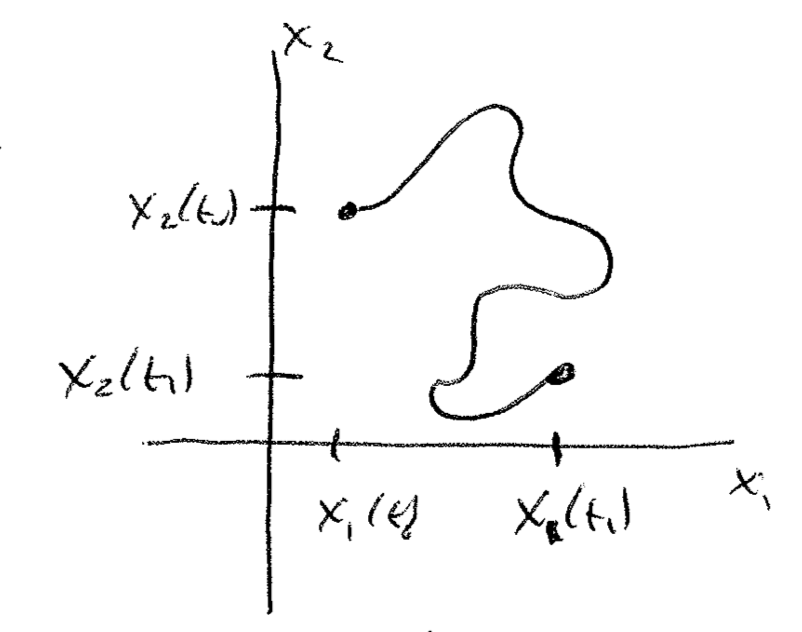
\includegraphics[scale=0.5]{22-1}
\end{center}
We call the $x_1, x_2$-plane the \underline{phase plane} for the system, noting that
\begin{enumerate}[label=\protect\circled{\alph*}]
	\item the independent variable $t$ is implicit to the graph (not an axis, but on the curve)
	\item For one equation $y' = f(y)$, the solution $y(t)$ lived in the $ty$-plane, but we could also track its evolution in the \underline{phase line}
	\item We could graph $\vec{x}(t)$ in the $tx_1 x_2$-space but this is hard to see.
\end{enumerate}
\subsubsection*{Some ideas for study}
\begin{enumerate}[label=\protect\circled{\Roman*}]
	\item $\vec{x}'(t) = A \vec{x}(t)$, by simply choosing points $\vec{x} \in \mathbb{R}^2$, we can plot tangent lines and make a slope field in the phase plane.
	\begin{example-N}
		Let $A = \begin{bmatrix}
			1 & 1\\ 6 & 0
		\end{bmatrix}$. Compute
		\begin{enumerate}[label=\protect\circled{\alph*}]
		\item $\vec{x} = \begin{bmatrix}
			1\\2
		\end{bmatrix}$, $\vec{x} = \begin{bmatrix}
			1 & 1\\ 6 & 0
		\end{bmatrix}
		\begin{bmatrix}
			1\\2
		\end{bmatrix} = 
		\begin{bmatrix}
			3\\6
		\end{bmatrix}$
		\item $\vec{x} = \begin{bmatrix}
			1\\0
		\end{bmatrix}$, $\vec{x} = \begin{bmatrix}
			1 & 1\\ 6 & 0
		\end{bmatrix}
		\begin{bmatrix}
			1\\0
		\end{bmatrix} = 
		\begin{bmatrix}
			1\\6
		\end{bmatrix}$\\
		\textbf{Notes: } 
			\begin{enumerate}[label=\protect\circled{\arabic*}]
			\item looks very similar to example 1
			\item Use JODE 2D calculator on website
			\end{enumerate}
	\end{enumerate}
	\end{example-N}
		\begin{center}
			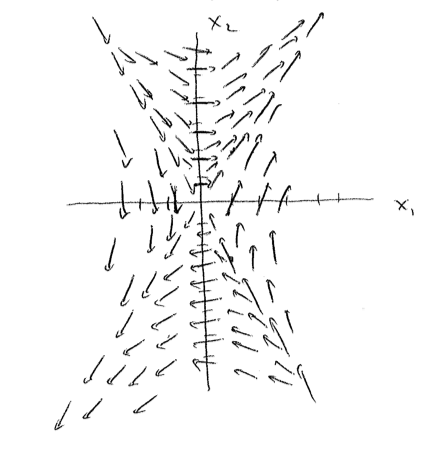
\includegraphics[scale=0.6]{22-2}
		\end{center}
	\item The solution curves will be integral curves of this slope field:
	\begin{enumerate}[label=\protect\circled{\alph*}]
	\item Given a value of $c_1, c_2 \in \mathbb{R}$, the curve $\vec{x(t)} = c_1 \begin{bmatrix}
				1\\2
			\end{bmatrix} e^{3t} + c_2
			\begin{bmatrix}
				1\\-3
			\end{bmatrix} e^{-2t}$ will be one of these curves.
	\item Straight line motion occurs when $c_1$ or $c_2 = 0$ 
	\end{enumerate}
\end{enumerate}
Choose $c_1 = -2, c_2 = 0$. then $\vec{x}(t) = -2 \begin{bmatrix}
	1\\2
\end{bmatrix} e^{3t} = \begin{bmatrix}
	-2\\-4
\end{bmatrix}e^{3t}$
\begin{center}
	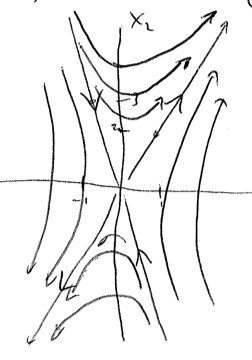
\includegraphics{22-3}
\end{center}
\classheader{2018-08-22}
For $\vec{x}' = A_{2x2}\vec{x}$,
\begin{enumerate}[label=\protect\circled{\Roman*}]
	\item One can construct a slope field in $\mathbb{R}^2$ via matrix multiplication: For $\vec{x} \in \mathbb{R}^2$, the tangent to the solution curve passing through is $\vec{x} = \begin{bmatrix}
		x_1\\ x_2
	\end{bmatrix}$ is $A\vec{x}$
	\begin{enumerate}[label=\protect\circled{\alph*}]
		\item $\vec{x} = \begin{bmatrix}
			1\\2
		\end{bmatrix}$, $\vec{x} = \begin{bmatrix}
			1 & 1\\ 6 & 0
		\end{bmatrix}
		\begin{bmatrix}
			1\\2
		\end{bmatrix} = 
		\begin{bmatrix}
			3\\6
		\end{bmatrix}$
		\item $\vec{x} = \begin{bmatrix}
			1\\0
		\end{bmatrix}$, $\vec{x} = \begin{bmatrix}
			1 & 1\\ 6 & 0
		\end{bmatrix}
		\begin{bmatrix}
			1\\0
		\end{bmatrix} = 
		\begin{bmatrix}
			1\\6
		\end{bmatrix}$
		\item $\vec{x} = \begin{bmatrix}
			0\\1
		\end{bmatrix}$, $\vec{x} = \begin{bmatrix}
			1 & 1\\ 6 & 0
		\end{bmatrix}
		\begin{bmatrix}
			0\\1
		\end{bmatrix} = 
		\begin{bmatrix}
			1\\0
		\end{bmatrix}$
	\end{enumerate}
	JODE 2D calculator or similar is helpful here.
	\item Solution curves are integral curves of the slope field:
	\begin{enumerate}[label=\protect\circled{\alph*}]
	\item Given $c_1, c_2 \in \mathbb{R}$, the curve $\vec{x(t)} = c_1 \begin{bmatrix}
				1\\2
			\end{bmatrix} e^{3t} + c_2
			\begin{bmatrix}
				1\\-3
			\end{bmatrix} e^{-2t}$ is one of these curves.
	\item Straight line motion only occurs when $c_1 = -2, c_2 = 0$. Then $\vec{x}(t) = -2 \begin{bmatrix}
	1\\2
\end{bmatrix} e^{3t} = \begin{bmatrix}
	-2\\-4
\end{bmatrix}e^{3t}$
	\item A copy of $\mathbb{R}^2$ with enough representative curve on it to give a sound sense of solutions is called a \underline{phase portrait}.
	\item Solutions are called \underline{trajectories} or \underline{orbits}.
	\item General long term behaviour of trajectories can be read off easily from a phase portrait:
	\begin{equation*}
		\text{Given } \quad \vec{x}(t) = c_1 \begin{bmatrix}
				1\\2
			\end{bmatrix} e^{3t} + c_2
			\begin{bmatrix}
				1\\-3
			\end{bmatrix} e^{-2t},
	\end{equation*}
	\begin{itemize}
		\item If $c_1 = 0$, $c_2 \neq 0$, then $\vec{x}(t) = c_2
			\begin{bmatrix}
				1\\-3
			\end{bmatrix} e^{-2t}$ and $\vec{x}(t) = c_2
			\begin{bmatrix}
				1\\-3
			\end{bmatrix} e^{-2t}$ and $\Lim{t \rightarrow \infty} \vec{x}(t) = \begin{bmatrix}
				0\\0
			\end{bmatrix}$ How about $\Lim{t \rightarrow -\infty} \vec{x}(t)?$ We say it is \underline{unbounded}.\\
		\textbf{Note: } Solutions never touch nor cross here. So since $\vec{x}(t) = \begin{bmatrix}
				0\\0
			\end{bmatrix}$ is in equilibrium solution, no other solution actually reader $\begin{bmatrix}
				0\\0
			\end{bmatrix}$
		\item If $c_1 \neq 0, c_2 = 0$?\\
		$\Lim{t \rightarrow \infty} \vec{x}(t)$ DNE on trig is unbounded\\
		$\Lim{t \rightarrow -\infty} \vec{x}(t) = \begin{bmatrix}
			0\\0
		\end{bmatrix}$
		\item If $c_1 \neq 0$ and $c_2 \neq 0$? These are the curved lines in the portrait. For these, what can we say about the forward trajectory ($\Lim{t \rightarrow \infty} \vec{x}(t)$), or the backward one ($\Lim{t \rightarrow -\infty} \vec{x}(t)$)?\\
		One Answer? Given $\quad \vec{x}(t) = c_1 \begin{bmatrix}
				1\\2
			\end{bmatrix} e^{3t} + c_2
			\begin{bmatrix}
				1\\-3
			\end{bmatrix} e^{-2t}$ and $c_1 \neq 0$, $c_2 \neq 0$, then as $t$ gets large $(t \rightarrow \infty)$, $\vec{x}(t)$ looks more and more like $c_1 \begin{bmatrix}
				1\\2
			\end{bmatrix} e^{3t}$, and less and less like $c_2
			\begin{bmatrix}
				1\\-3
			\end{bmatrix} e^{-2t}$. How about in backward time?
	\end{itemize}
	\begin{center}
		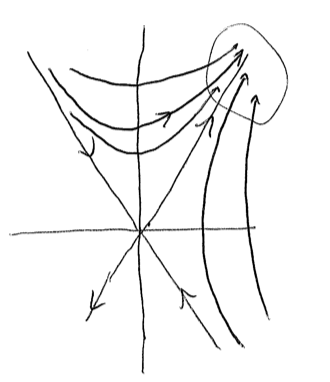
\includegraphics{23-1}
	\end{center}
	\end{enumerate}
	\item Back to solution building via properties of A: For $\vec{x} = \begin{bmatrix}
			1 & 1\\ 6 & 0
		\end{bmatrix} \vec{x}$, 
		\begin{equation*}
			\vec{x}(t) = c_1 \begin{bmatrix}
				1\\2
			\end{bmatrix} e^{3t} + c_2
			\begin{bmatrix}
				1\\-3
			\end{bmatrix} e^{-2t}
		\end{equation*}
		the eigenvalues of A ($\Gamma_1 = 3, \Gamma_2 = -2$), and representive eigenvectors ($\vec{v_1} = \begin{bmatrix}
			1\\2
		\end{bmatrix}, \vec{v_2} = \begin{bmatrix}
			1\\-3
		\end{bmatrix}$) are explicitly part of the solution. \underline{Why?}\\
		Here, the eigenvalues and eigenvectors of a matrix $A$ satisfy $A\vec{v} = \lambda \vec{v}$, or $(A - \lambda I)\vec{v} = \vec{0}$\\
		For this to have non trivial solutions for $\vec{v}$,
		\begin{itemize}
			\item $\lambda$ must be an eigenvalue, and 
			\item $\det (A - \lambda I) \vec{v} = \vec{0}$
		\end{itemize}
		For $A = \begin{bmatrix}
			a& b\\ c& d
		\end{bmatrix}, \det (A- \lambda I) = \begin{vmatrix}
			a - \lambda & b\\
			c & d - \lambda
		\end{vmatrix} = 0$\\
		$ = \lambda^2 - (a + d)\lambda + (ad - bc) = 0$\\
		This is called the \underline{characteristic equation} of A, and solutions can be
		\begin{enumerate}[label=\protect\circled{\arabic*}]
		\item real, distinct
		\item real and repeated
		\item complex conjugates
		\end{enumerate}
		How to relate to solutions of $\vec{x}' = A\vec{x}$?
		\begin{itemize}
			\item Recall $\dot{x} = ax$ is solved by $x(t) = ce^{at}$
			\item Assume $\dot{\vec{x}} = A\vec{x}$ is also solved by exponentials. For $n=2$, $\vec{x} = \begin{bmatrix}
				x_1 \\x_2
			\end{bmatrix}$. Assume $x_1(t) = c_1e^{\Gamma t}$, $x_2(t) = c_2e^{\Gamma t}$\\
			$\Rightarrow \vec{x}(t) = \begin{bmatrix}
				c_1\\c_2
			\end{bmatrix} e^{\Gamma t}$, and $\vec{x}' = \Gamma \begin{bmatrix}
				c_1\\c_2
			\end{bmatrix} e^{\Gamma t}$ and then $\vec{x}' = A \vec{x}$ is $\Gamma \begin{bmatrix}
				c_1\\c_2
			\end{bmatrix} e^{\Gamma t} = A \begin{bmatrix}
				c_1\\c_2
			\end{bmatrix} e^{\Gamma t}$ or $\Gamma \begin{bmatrix}
				c_1\\c_2
			\end{bmatrix}  = A \begin{bmatrix}
				c_1\\c_2
			\end{bmatrix}$, is $\Gamma \vec{v} = A\vec{v}$.\\
			And what do solutions to this look like? 
			\begin{itemize}
			\item $\Gamma$ is an eigenvalue
			\item $\vec{v}$ is an eigenvector of $\Gamma$.
			\end{itemize}
		\end{itemize}
		\textbf{Notes: }
		\begin{enumerate}[label=\protect\circled{\arabic*}]
		\item This works equally well for $n > 2$.
		\item In the case where $A_{nxn}$ is real and symmetric (i.e. when $a_{ij} = a_{ji}$)\\
		$\Rightarrow$ all eigenvalues one real and even if repeated, there is a full set of eigenvectors.
		\end{enumerate}
		We have the following:\\
		For $\dot{\vec{x}} = A_{nxn} \vec{x}$, when all eigenvalues of A are real and distinct, then
		\begin{equation*}
			\vec{x}(t) = c_1\vec{v_1}e^{\Gamma_1 t} + \cdots + c_n\vec{v_n}e^{\Gamma_n t}
		\end{equation*}
		is the general solution, where $\vec{v_i}$ is on eigenvector of $\Gamma_i$ for A.
\end{enumerate}
\classheader{2018-08-22}
Back to $\vec{x}' = A_{2x2} \vec{x}$ in the case where the 2 eigenvalues of $A, \Gamma_1, \Gamma_2$ are real and distinct: $\Gamma_1 \neq \Gamma_2$\\
\textbf{Some Notes: }
\begin{enumerate}[label=\protect\circled{\arabic*}]
	\item This works fine when 0 is an eigenvalue
	\begin{example-N}
		$\vec{x}' = \begin{bmatrix}
			3 & -3\\
			1 & -1
		\end{bmatrix} \vec{x}$. Here characteristic equation is $\Gamma^2 - 2\Gamma = 0$, w/ solutions $\Gamma_1 = 0$, $\Gamma_2 = 2$.\\
		For $\Gamma_1 = 0$, $\vec{v_1} = \begin{bmatrix}
			1\\1
		\end{bmatrix}$ is a choice of eigenvector\\
		For $\Gamma_2 = 2$, $\vec{v_2} = \begin{bmatrix}
			3\\1
		\end{bmatrix}$ is one choice\\
		Then $\vec{x}(t) = c_1\vec{v_1}e^{\Gamma_1 t} + c_2\vec{v_2}e^{\Gamma_2 t} = \boxed{c_1 \begin{bmatrix}
			1\\1
		\end{bmatrix} + c_2 \begin{bmatrix}
			1\\1
		\end{bmatrix} e^{2t}}$ is general solution.
	\end{example-N}
	\textbf{Question:} So what does the phase portrait look like here?
	\begin{center}
		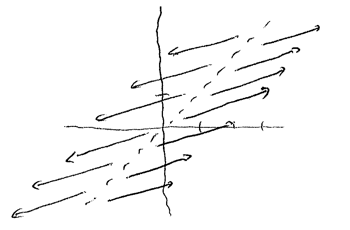
\includegraphics{24-1}
	\end{center}
	\item This formulation of the general solution still works even for repeated eigenvalues \underline{if}	 there are enough eigenvectors.
	\begin{example-N}
		$\vec{x}' = \begin{bmatrix}
			1 & 0 \\ 0 & 1
		\end{bmatrix} \vec{x}$. Here characteristic equation is $\Gamma^2 - 2\Gamma + 1 = 0 = (\Gamma - 1)^2$. Hence $\Gamma_1 = \Gamma_2 = 1$.\\
		The eigenvector equation $\begin{bmatrix}
			1 & 0 \\ 0 & 1
		\end{bmatrix} \begin{bmatrix}
			x_1 \\ x_2
		\end{bmatrix} = 1 \begin{bmatrix}
			x_1\\x_2
		\end{bmatrix}$\\
		One choice is $\vec{v_1} = \begin{bmatrix}
			1 \\ 0 
		\end{bmatrix}, \vec{v_2} = \begin{bmatrix}
			0 \\ 1
		\end{bmatrix}$
		\begin{equation*}
			\text{Hence } \vec{x}(t) = c_1 \begin{bmatrix}
			1 \\ 0 
		\end{bmatrix} e^t + c_2 \begin{bmatrix}
			0 \\ 1 
		\end{bmatrix} e^t \text{ is the general solution}
		\end{equation*} 
	\end{example-N}
	\begin{example-N}
		$\vec{x}' = \begin{bmatrix}
			0 & 1 & 1\\
			1 & 0 & 1\\
			1 & 1 & 0
		\end{bmatrix} \vec{x}$\\
		Here $A = \begin{bmatrix}
			0 & 1 & 1\\
			1 & 0 & 1\\
			1 & 1 & 0
		\end{bmatrix}$ and the characteristic equation after $\det (A - \Gamma I)$ is $\boxed{(\Gamma + 1)^2 (\Gamma -2)}$. The eigenvalues are $\Gamma_1 = 2$, $\Gamma_2 = \Gamma_3 = -1$\\
		The respective eigenvectors are
		$\vec{v_1} = \begin{bmatrix}
			1\\1\\1
		\end{bmatrix}$, $\vec{v_2} = \begin{bmatrix}
			1\\0\\-1
		\end{bmatrix}$, $\vec{v_3} = \begin{bmatrix}
			0\\1\\-1
		\end{bmatrix}$\\
		So the general solution is 
		\begin{equation*}
			\vec{x}(t) = c_1 \begin{bmatrix}
			1\\1\\1
		\end{bmatrix} e^{2t} + c_2 \begin{bmatrix}
			1\\0\\-1
		\end{bmatrix} e^{-t} + c_3
		\begin{bmatrix}
			0\\1\\-1
		\end{bmatrix} e^{-t}
		\end{equation*}
	\end{example-N}
	\item  This formulation for finding solution \underline{does not} work when there are not enough independent eigenvectors for repeated eigenvalues
	\begin{example-N}
		$\vec{x}' = \begin{bmatrix}
			-2 & 1\\
			0 & -2
		\end{bmatrix} \vec{x}$. Here eigenvalues are $\Gamma_1 = \Gamma_2 = -2$. But the eigenvector equation $A\vec{v} = -2\vec{v}$, or
		\begin{align*}
			-2x_1 + x_2 & = -2x_2\\
			-2x_2 & = -2x_2
		\end{align*}
		is \underline{only} solved by $x_2 = 0$, $x_2 \neq 0$. Then only independent choice would be $\vec{v} = \begin{bmatrix}
			1\\0
		\end{bmatrix}$\\
	\end{example-N}
	Here, we will need to come up with another method to find another independent solution.
\end{enumerate}
\subsubsection*{Properties of phase portraits}
let $\vec{x}' = A\vec{x}$. We have
\begin{enumerate}[label=\protect\circled{\arabic*}]
	\item For \underline{any} $A_{2x2}$, the origin is an equilibrium solution ($\vec{x} = \begin{bmatrix}
		0\\0
	\end{bmatrix}$ is always a solution to $A\vec{x} = \vec{0}$).
	\item If $\det A \neq 0$, then $\vec{x} = \begin{bmatrix}
		0\\0
	\end{bmatrix}$ is the \underline{ONLY} equilibrium solution (\underline{stationary point}, or \underline{fixed point}), since $A\vec{x} = \vec{0}$ has $\begin{bmatrix}
		0\\0
	\end{bmatrix}$ as the only solution.
	\item The eigenvectors of $A$ correspond to lines through the origin where the solutions exhibit straight line motion\\
	\textbf{Note: } These straight lines contain many distinct solutions.
	\item The sign of each eigenvalue determines direction along lines (towered origin if $<0$ outward if $>0$).
	\item If eigenvalues are real and distinct then there are the only straight lines (why?)
	\item Signs of eigenvalues determine "stability" of equilibrium at origin. (How solutions behave "near" the origin. Do they stay nearby, converse to, or diverse from...)
	\item Below, origin is called a \underline{"saddle point"} . Would you consider it saddle?
\end{enumerate}
\begin{example-N}
	$\vec{x} = \begin{bmatrix}
		-4 & 1\\
		3 & -2
	\end{bmatrix} \vec{x} \quad \quad$ Here $\Gamma_1 = -5, \Gamma_2 = -1$, with $\vec{v}_1 = \begin{bmatrix}
		-1 \\1
	\end{bmatrix}, \vec{v}_2 = \begin{bmatrix}
		1 \\3
	\end{bmatrix}$\\
	General solution is $\vec{x}(t) = c_1 \begin{bmatrix}
		-1 \\1
	\end{bmatrix} e^{-5t} + c_2 \begin{bmatrix}
		1 \\3
	\end{bmatrix} e^{-t}$. Phase portrait is similar to above but different: how?\\
	Here origin is a "sink" and asymptotically stable.
	\begin{center}
		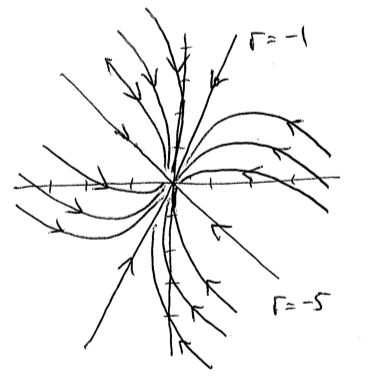
\includegraphics[scale=0.6]{24-2}
	\end{center}
\end{example-N}
\begin{example-N}
	$\vec{x} = \begin{bmatrix}
		1 & 0\\
		0 & 1
	\end{bmatrix} \vec{x} \quad \quad$ Here, as we have seen $\Gamma_1 = \Gamma_2 = 1$, $\vec{v_1} = \begin{bmatrix}
		1\\0
	\end{bmatrix}, \vec{v_2} = \begin{bmatrix}
		0\\1
	\end{bmatrix}$ and General solution is $\vec{x}(t) = c_1 \begin{bmatrix}
		1\\0
	\end{bmatrix}e^t + c_2 \begin{bmatrix}
		0\\1
	\end{bmatrix} e^t = \bigg( c_1 \begin{bmatrix}
		1\\0
	\end{bmatrix} + c_2 \begin{bmatrix}
		0\\1
	\end{bmatrix} \bigg)e^t$.\\
	This is another sources at the origin hhere called a \underline{star node}
	\begin{center}
		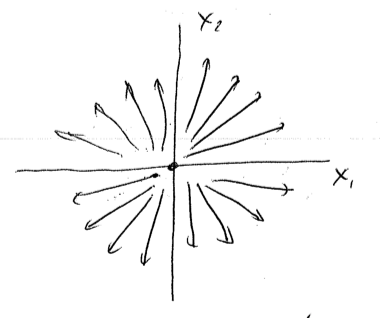
\includegraphics[scale=0.7]{24-3}
	\end{center}
\end{example-N}
\begin{example-N}
	$\vec{x} = \begin{bmatrix}
		3 & -3\\
		1 & -1
	\end{bmatrix} \vec{x} \quad \quad$ Here $\Gamma_1 = 0, \Gamma_2 = 2$, $\vec{v_1} = \begin{bmatrix}
		1\\1
	\end{bmatrix}, \vec{v_2} = \begin{bmatrix}
		3\\1
	\end{bmatrix}$ and General solution is $\vec{x}(t) = c_1 \begin{bmatrix}
		1\\2
	\end{bmatrix} + c_2 \begin{bmatrix}
		3\\1
	\end{bmatrix} e^{2t}$\\
	This one is special: There is a line of equilibrium solution (determinant is 0). Off the dotted line, motion is straight along lines parallel to $\begin{bmatrix}
		3\\1
	\end{bmatrix}$ and moving out from dotted line.
	\begin{center}
		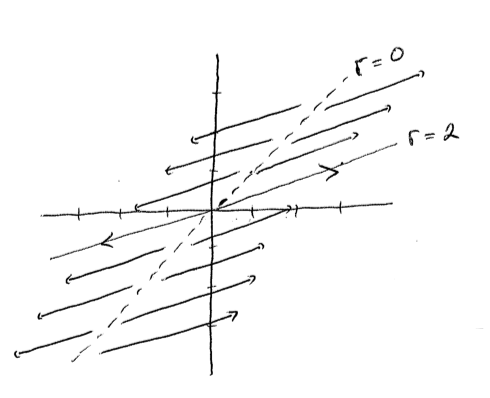
\includegraphics[scale=0.6]{24-5}
	\end{center}
\end{example-N}
\classheader{2018-08-29}
\subsection*{Complex Eigenvalues}
\textbf{New Question:} What is the eigenvalues (solutions to the \underline{characteristic equation} of $A_{2x2}$ in $\vec{x}' = A\vec{x}$) are not real?\\
Then They are complex (the discriminant $b^2 - 4ac$ of the quadratic formula used to solve the \underline{characteristic equation} is < 0).\\
They must be complex conjugates (why?) How to use them?
Let's play the same game for constructing solutions to $\vec{x}' = A\vec{x}$ using eigenvalue eigenvector pairs:\\
For $\vec{x}' = A_{2x2} \vec{x}$, suppose $\Gamma_1 \neq \Gamma_2$ are two distinct solutions to characteristic equation of $A$ and we calculate eigenvectors $\vec{v_1}, \vec{v_2}$ respectively to $\Gamma_1, \Gamma_2$. Then general solution is
\begin{equation*}
	\tcbhighmath[drop fuzzy shadow]{\vec{x}(t) = c_1 \vec{v_1} e^{\Gamma_1 t} + c_2 \vec{v_2} e^{\Gamma_2 t}}
\end{equation*}
We try this with complex $\Gamma$:
\begin{example-N}
	$\vec{x}' = \begin{bmatrix}
		0 & 1\\
		-2 & -2
	\end{bmatrix} \vec{x} \quad$ Characteristic equation is $\Gamma^2 + 2\Gamma + 2 = 0$, solved by $\Gamma = -1 \pm i$\\
	Leave them as $\Gamma_1 = -1 + i$, $\Gamma_2 = -1-i$ and solve for $\vec{v_1}$: $A\vec{v} = \Gamma \vec{v}$
	\begin{gather*}
		\begin{bmatrix}
			0 & 1\\
			-2 & -2
		\end{bmatrix}
		\begin{bmatrix}
			v_1\\
			v_2
		\end{bmatrix} = (-1 + i)
		\begin{bmatrix}
			v_1\\
			v_2
		\end{bmatrix}\\
		v_2 = -v_1 + iv_1\\
		-2v_1 -2v_2 = -v_2 + iv_2
	\end{gather*}
\end{example-N}
We can substitute $(1)$ into $(2)$ and simplify to get $-2iv_1 = -2iv_1$, solved by any choice of v. For example, choose $v_1 = 1$. Then $v_1 = (-1+i)$ and 
\begin{equation*}
	\Gamma_1 -1 + i, \quad \vec{v_1} = \begin{bmatrix}
		1\\
		-1 + i
	\end{bmatrix} \quad \quad \text{forms an "eigenvalue/eigenvector" pair}
\end{equation*}
\textbf{Notes:}
\begin{enumerate}[label=\protect\circled{\arabic*}]
	\item This is not quite accurate since the definition of eigenvector is that of a vector whose direction does not change upon multiplication by a matrix. Without real eigenvalues, there are no real eigenvectors! But the term "complex eigenvector" is a commonly used one. 
	\item The other eigenvalue/eigenvector pair is $\Gamma_2 = -1 -i, \quad \vec{v_1} = \begin{bmatrix}
		1\\
		-1 - i
	\end{bmatrix}$
	\item Rewrite $\vec{v_1} = \begin{bmatrix}
		1\\
		-1 + i
	\end{bmatrix} = \begin{bmatrix}
		1\\-1
	\end{bmatrix} + \begin{bmatrix}
		0\\1
	\end{bmatrix}i = \vec{a} + i\vec{b}$. Then along with $\Gamma_1 = -1 + i = \lambda + i \mu$ we can attempt to form solutions.
\end{enumerate}
General idea for a Method for constructing solutions?\\
\redhline\\\\
Given:
\begin{itemize}
	\item $\Gamma_1 = \lambda + i \mu$, $\vec{v_1} = \vec{a} + i \vec{b}$
	\item $\Gamma_1 = \lambda - i \mu$, $\vec{v_1} = \vec{a} - i \vec{b}$
\end{itemize}
Create a "complex" solution in the normal way:
\begin{align*}
	\vec{x}(t) & = \vec{v_1}e^{\Gamma_1 t} = (\vec{a} + i\vec{b}) \underbrace{e^{\lambda t}(\cos \mu t) + i \sin \mu t}_{\text{Euler formula for } e^{\Gamma_1 t}}\\
	& = e^{\lambda t}(\vec{a} \cos \mu t - \vec{b} \sin \mu t) + ie^{\lambda t}(\vec{a}\sin \mu t + \vec{b} \cos t)
\end{align*}
Hence we can write $\vec{x}(t) = \vec{a}(t) + i \vec{w}(t)$, where
\begin{gather*}
	\vec{u}(t) = e^{\lambda t}(\vec{a} \cos \mu t - \vec{b} \sin \mu t)\\
	\vec{u}(t) = e^{\lambda t}(\vec{a} \sin \mu t - \vec{b} \cos \mu t)
\end{gather*}
\underline{Notes: }
\begin{enumerate}[label=\protect\circled{\arabic*}]
	\item These are 2 real-valued functions which each solve the ODE $\vec{x}' = A \vec{x}$ (check this!)
	\item These are independent (check the Wronskian)
	\item The general solution to $\vec{x}' = A\vec{x}$ when eigenvalues $\Gamma = \lambda \pm i \mu$ are complex and with eigenvectors $\vec{v} = \vec{a} \pm i \vec{b}$ is 
\begin{equation*}
	\vec{x}(t) = c_1 \vec{u}(t) + c_2 \vec{w}(t)
\end{equation*}
\end{enumerate}
\redhline\\\\
\underline{Back to example:} $\vec{x}' = \begin{bmatrix}
	0 & 1\\
	-2 & -2
\end{bmatrix} \vec{x}$.\\
Here $\Gamma_1 = \lambda + i \mu = -1 + i$, $\vec{v_1} = \vec{a} + i \vec{b} = \begin{bmatrix}
	1\\-1
\end{bmatrix} + i \begin{bmatrix}
	0\\1
\end{bmatrix}$\\ So\\
\begin{equation*}
	\vec{x}(t) = c_1 e^{-t} \bigg( \begin{bmatrix}
		1\\ -1
	\end{bmatrix} \cos t - \begin{bmatrix}
		0\\1
	\end{bmatrix} \sin t \bigg) + c_2 e^{-t} \bigg( \begin{bmatrix}
		-1\\ 1
	\end{bmatrix} \sin t - \begin{bmatrix}
		0\\1
	\end{bmatrix} \cos t \bigg) 
\end{equation*}
\classheader{2018-08-29}

\classheader{2018-09-05}
Recall our fundamental set of solutions to
\begin{equation*}
	\vec{x}' = \begin{bmatrix}
		1 & 1\\ 6 & 0
	\end{bmatrix} \vec{x} \qquad \text{is} \qquad \Xlines(t) = \begin{bmatrix}
		e^{3t} & e^{-2t}\\
		2e^{3t} & -3e^{-2t}
	\end{bmatrix}
\end{equation*}
where the columns of $\Xlines(t)$ correspond to the 2 independent solutions
\begin{equation*}
	\vec{x}^{(1)}(t) = \begin{bmatrix}
		1 \\ 2
	\end{bmatrix} e^{3t}, \qquad \vec{x}^{(2)}(t) = \begin{bmatrix}
		1 \\ -3
	\end{bmatrix} e^{-2t}
\end{equation*}
They are independent, since $\det \Xlines(t) \neq 0$\\
The general solution is then\\
\begin{gather*}
	\vec{x}(t) = c_1 \begin{bmatrix}
		1 \\ 2
	\end{bmatrix} e^{3t} + c_2 \begin{bmatrix}
		1 \\ -3
	\end{bmatrix} e^{-2t}\\
	\begin{bmatrix}
		x_1(t)\\
		x_2(t)
	\end{bmatrix} = 
	\begin{bmatrix}
		c_1 e^{3t} + c_2 e^{-2t}\\
		2c_1 e^{3t} - 3c_2 e^{-2t}
	\end{bmatrix} = 
	\begin{bmatrix}
		e^{3t} & e^{-2t}\\
		2e^{3t} & -3e^{-2t}
	\end{bmatrix} 
	\begin{bmatrix}
		c_1\\
		c_2
	\end{bmatrix}
\end{gather*}
\begin{equation*}
	\vec{x}(t) = \Xlines(t)\vec{c}, \qquad \text{where} \quad \vec{c} = \begin{bmatrix}
	c_1\\
	c_2
	\end{bmatrix}
\end{equation*}
Here, given any initial data, $\vec{x}(t_0) = \vec{x}^0 = \begin{bmatrix}
	x_1^0\\
	x_2^0
\end{bmatrix}$






	
\end{document}
